\documentclass[twoside]{book}

% Packages required by doxygen
\usepackage{fixltx2e}
\usepackage{calc}
\usepackage{doxygen}
\usepackage[export]{adjustbox} % also loads graphicx
\usepackage{graphicx}
\usepackage[utf8]{inputenc}
\usepackage{makeidx}
\usepackage{multicol}
\usepackage{multirow}
\PassOptionsToPackage{warn}{textcomp}
\usepackage{textcomp}
\usepackage[nointegrals]{wasysym}
\usepackage[table]{xcolor}

% Font selection
\usepackage[T1]{fontenc}
\usepackage[scaled=.90]{helvet}
\usepackage{courier}
\usepackage{amssymb}
\usepackage{sectsty}
\renewcommand{\familydefault}{\sfdefault}
\allsectionsfont{%
  \fontseries{bc}\selectfont%
  \color{darkgray}%
}
\renewcommand{\DoxyLabelFont}{%
  \fontseries{bc}\selectfont%
  \color{darkgray}%
}
\newcommand{\+}{\discretionary{\mbox{\scriptsize$\hookleftarrow$}}{}{}}

% Page & text layout
\usepackage{geometry}
\geometry{%
  a4paper,%
  top=2.5cm,%
  bottom=2.5cm,%
  left=2.5cm,%
  right=2.5cm%
}
\tolerance=750
\hfuzz=15pt
\hbadness=750
\setlength{\emergencystretch}{15pt}
\setlength{\parindent}{0cm}
\setlength{\parskip}{0.2cm}
\makeatletter
\renewcommand{\paragraph}{%
  \@startsection{paragraph}{4}{0ex}{-1.0ex}{1.0ex}{%
    \normalfont\normalsize\bfseries\SS@parafont%
  }%
}
\renewcommand{\subparagraph}{%
  \@startsection{subparagraph}{5}{0ex}{-1.0ex}{1.0ex}{%
    \normalfont\normalsize\bfseries\SS@subparafont%
  }%
}
\makeatother

% Headers & footers
\usepackage{fancyhdr}
\pagestyle{fancyplain}
\fancyhead[LE]{\fancyplain{}{\bfseries\thepage}}
\fancyhead[CE]{\fancyplain{}{}}
\fancyhead[RE]{\fancyplain{}{\bfseries\leftmark}}
\fancyhead[LO]{\fancyplain{}{\bfseries\rightmark}}
\fancyhead[CO]{\fancyplain{}{}}
\fancyhead[RO]{\fancyplain{}{\bfseries\thepage}}
\fancyfoot[LE]{\fancyplain{}{}}
\fancyfoot[CE]{\fancyplain{}{}}
\fancyfoot[RE]{\fancyplain{}{\bfseries\scriptsize Generated by Doxygen }}
\fancyfoot[LO]{\fancyplain{}{\bfseries\scriptsize Generated by Doxygen }}
\fancyfoot[CO]{\fancyplain{}{}}
\fancyfoot[RO]{\fancyplain{}{}}
\renewcommand{\footrulewidth}{0.4pt}
\renewcommand{\chaptermark}[1]{%
  \markboth{#1}{}%
}
\renewcommand{\sectionmark}[1]{%
  \markright{\thesection\ #1}%
}

% Indices & bibliography
\usepackage{natbib}
\usepackage[titles]{tocloft}
\setcounter{tocdepth}{3}
\setcounter{secnumdepth}{5}
\makeindex

% Hyperlinks (required, but should be loaded last)
\usepackage{ifpdf}
\ifpdf
  \usepackage[pdftex,pagebackref=true]{hyperref}
\else
  \usepackage[ps2pdf,pagebackref=true]{hyperref}
\fi
\hypersetup{%
  colorlinks=true,%
  linkcolor=blue,%
  citecolor=blue,%
  unicode%
}

% Custom commands
\newcommand{\clearemptydoublepage}{%
  \newpage{\pagestyle{empty}\cleardoublepage}%
}


%===== C O N T E N T S =====

\begin{document}

% Titlepage & ToC
\hypersetup{pageanchor=false,
             bookmarks=true,
             bookmarksnumbered=true,
             pdfencoding=unicode
            }
\pagenumbering{roman}
\begin{titlepage}
\vspace*{7cm}
\begin{center}%
{\Large Glex \\[1ex]\large 2 }\\
\vspace*{1cm}
{\large Generated by Doxygen 1.8.10}\\
\end{center}
\end{titlepage}
\clearemptydoublepage
\tableofcontents
\clearemptydoublepage
\pagenumbering{arabic}
\hypersetup{pageanchor=true}

%--- Begin generated contents ---
\chapter{Hierarchical Index}
\section{Class Hierarchy}
This inheritance list is sorted roughly, but not completely, alphabetically\+:\begin{DoxyCompactList}
\item \contentsline{section}{Bounding\+Box}{\pageref{class_bounding_box}}{}
\item \contentsline{section}{Camera}{\pageref{class_camera}}{}
\item \contentsline{section}{Game\+Asset}{\pageref{class_game_asset}}{}
\begin{DoxyCompactList}
\item \contentsline{section}{Cube\+Asset}{\pageref{class_cube_asset}}{}
\item \contentsline{section}{Diamond\+Asset}{\pageref{class_diamond_asset}}{}
\item \contentsline{section}{Grass\+Asset}{\pageref{class_grass_asset}}{}
\item \contentsline{section}{Ground\+Asset}{\pageref{class_ground_asset}}{}
\item \contentsline{section}{Leaves\+Asset}{\pageref{class_leaves_asset}}{}
\item \contentsline{section}{Pyramid\+Asset}{\pageref{class_pyramid_asset}}{}
\end{DoxyCompactList}
\item \contentsline{section}{Game\+Asset\+Manager}{\pageref{class_game_asset_manager}}{}
\item \contentsline{section}{Game\+Loop}{\pageref{class_game_loop}}{}
\item \contentsline{section}{Game\+World}{\pageref{class_game_world}}{}
\item \contentsline{section}{Python\+Bind}{\pageref{class_python_bind}}{}
\item \contentsline{section}{S\+D\+L\+Window\+Deleter}{\pageref{struct_s_d_l_window_deleter}}{}
\end{DoxyCompactList}

\chapter{Class Index}
\section{Class List}
Here are the classes, structs, unions and interfaces with brief descriptions\+:\begin{DoxyCompactList}
\item\contentsline{section}{\hyperlink{class_bounding_box}{Bounding\+Box} }{\pageref{class_bounding_box}}{}
\item\contentsline{section}{\hyperlink{class_camera}{Camera} }{\pageref{class_camera}}{}
\item\contentsline{section}{\hyperlink{class_cube_asset}{Cube\+Asset} }{\pageref{class_cube_asset}}{}
\item\contentsline{section}{\hyperlink{class_diamond_asset}{Diamond\+Asset} }{\pageref{class_diamond_asset}}{}
\item\contentsline{section}{\hyperlink{class_game_asset}{Game\+Asset} }{\pageref{class_game_asset}}{}
\item\contentsline{section}{\hyperlink{class_game_asset_manager}{Game\+Asset\+Manager} }{\pageref{class_game_asset_manager}}{}
\item\contentsline{section}{\hyperlink{class_game_loop}{Game\+Loop} }{\pageref{class_game_loop}}{}
\item\contentsline{section}{\hyperlink{class_game_world}{Game\+World} }{\pageref{class_game_world}}{}
\item\contentsline{section}{\hyperlink{class_grass_asset}{Grass\+Asset} }{\pageref{class_grass_asset}}{}
\item\contentsline{section}{\hyperlink{class_ground_asset}{Ground\+Asset} }{\pageref{class_ground_asset}}{}
\item\contentsline{section}{\hyperlink{class_leaves_asset}{Leaves\+Asset} }{\pageref{class_leaves_asset}}{}
\item\contentsline{section}{\hyperlink{class_pyramid_asset}{Pyramid\+Asset} }{\pageref{class_pyramid_asset}}{}
\item\contentsline{section}{\hyperlink{class_python_bind}{Python\+Bind} }{\pageref{class_python_bind}}{}
\item\contentsline{section}{\hyperlink{struct_s_d_l_window_deleter}{S\+D\+L\+Window\+Deleter} }{\pageref{struct_s_d_l_window_deleter}}{}
\end{DoxyCompactList}

\chapter{Class Documentation}
\hypertarget{class_bounding_box}{}\section{Bounding\+Box Class Reference}
\label{class_bounding_box}\index{Bounding\+Box@{Bounding\+Box}}


{\ttfamily \#include $<$Bounding\+Box.\+h$>$}

\subsection*{Public Member Functions}
\begin{DoxyCompactItemize}
\item 
\hyperlink{class_bounding_box_ab5c42370640606c132b4b797cb0c7c2f}{Bounding\+Box} (glm\+::vec3 xyz\+Position, glm\+::vec3 translate\+To, glm\+::vec3 animate\+To, bool translate\+\_\+bool, glm\+::vec3 rotate, bool rotate\+\_\+bool, glm\+::vec3 scale, bool scale\+\_\+bool, string \&Asset\+Type)
\item 
glm\+::mat4 \hyperlink{class_bounding_box_a5fd1769f7157e7df40a6ab6a242fcfcc}{Get\+Model} ()
\item 
void \hyperlink{class_bounding_box_a9898275b1cd97761855156fc965412b1}{Translate\+X} ()
\item 
void \hyperlink{class_bounding_box_aedff87fb2721b1e706e6e033e35b676b}{Translate\+Y} ()
\item 
void \hyperlink{class_bounding_box_a33d133625c7a1a6f6dd7628f00388fd5}{Translate\+Z} ()
\item 
void \hyperlink{class_bounding_box_a728a3700574a5d9fbcac6d94561336ed}{Rotate} (glm\+::vec3 rotate)
\item 
void \hyperlink{class_bounding_box_ab84e48c88a509b20a469ccf5e23c4f11}{Scale} (glm\+::vec3 scale)
\item 
glm\+::vec3 \hyperlink{class_bounding_box_a45332d45575fe93b516267436abcd4fe}{Get\+Translate\+To} ()
\item 
bool \hyperlink{class_bounding_box_a501c1fd40b00ce6295fd60e1ed8cd92c}{Get\+Translate\+Bool} ()
\item 
bool \hyperlink{class_bounding_box_a262907e4b68e555edc57b21faef5685b}{Get\+Scale\+Bool} ()
\item 
bool \hyperlink{class_bounding_box_a6686a674cd3de57c987bccdfe6acbe92}{Get\+Rotate\+Bool} ()
\item 
glm\+::vec3 \hyperlink{class_bounding_box_a9d1fe341d5c2033e7f20ab9bdb4ae4b9}{Get\+A\+A\+B\+B} (string check)
\item 
void \hyperlink{class_bounding_box_a158978699951663552a2936f2a8a2339}{Collision\+Detection} (glm\+::vec3 B\+B1\+\_\+\+Max, glm\+::vec3 B\+B1\+\_\+\+Min, glm\+::vec3 B\+B1\+\_\+\+Pos, glm\+::vec3 B\+B2\+\_\+\+Max, glm\+::vec3 B\+B2\+\_\+\+Min, glm\+::vec3 B\+B2\+\_\+\+Pos)
\end{DoxyCompactItemize}


\subsection{Constructor \& Destructor Documentation}
\hypertarget{class_bounding_box_ab5c42370640606c132b4b797cb0c7c2f}{}\index{Bounding\+Box@{Bounding\+Box}!Bounding\+Box@{Bounding\+Box}}
\index{Bounding\+Box@{Bounding\+Box}!Bounding\+Box@{Bounding\+Box}}
\subsubsection[{Bounding\+Box(glm\+::vec3 xyz\+Position, glm\+::vec3 translate\+To, glm\+::vec3 animate\+To, bool translate\+\_\+bool, glm\+::vec3 rotate, bool rotate\+\_\+bool, glm\+::vec3 scale, bool scale\+\_\+bool, string \&\+Asset\+Type)}]{\setlength{\rightskip}{0pt plus 5cm}Bounding\+Box\+::\+Bounding\+Box (
\begin{DoxyParamCaption}
\item[{glm\+::vec3}]{xyz\+Position, }
\item[{glm\+::vec3}]{translate\+To, }
\item[{glm\+::vec3}]{animate\+To, }
\item[{bool}]{translate\+\_\+bool, }
\item[{glm\+::vec3}]{rotate, }
\item[{bool}]{rotate\+\_\+bool, }
\item[{glm\+::vec3}]{scale, }
\item[{bool}]{scale\+\_\+bool, }
\item[{string \&}]{Asset\+Type}
\end{DoxyParamCaption}
)}\label{class_bounding_box_ab5c42370640606c132b4b797cb0c7c2f}
Initalise Data The below vectors and booleans initialise all the variables used in the bounding box class to calculate and animate the Bounding Box 
\begin{DoxyCode}
5                                                                             \{
11         this->xyzPosition = xyzPosition;
12         this->translateTo = translateTo;
13         translateToSave = translateTo;
14         this->animateTo = animateTo;
15         this->translate\_bool = translate\_bool;
16 
17         this->rotate = rotate;
18         rotateTo = rotate;
19         this->rotate\_bool = rotate\_bool;
20  
21         this->scale = scale;
22         scaleTo = scale;
23         this->scale\_bool = scale\_bool;
24         this->AssetType = AssetType;
25 
26         cout << \textcolor{stringliteral}{"Bounding Box Created at: "} << glm::to\_string(translateTo)<< endl;
27 \}
\end{DoxyCode}


\subsection{Member Function Documentation}
\hypertarget{class_bounding_box_a158978699951663552a2936f2a8a2339}{}\index{Bounding\+Box@{Bounding\+Box}!Collision\+Detection@{Collision\+Detection}}
\index{Collision\+Detection@{Collision\+Detection}!Bounding\+Box@{Bounding\+Box}}
\subsubsection[{Collision\+Detection(glm\+::vec3 B\+B1\+\_\+\+Max, glm\+::vec3 B\+B1\+\_\+\+Min, glm\+::vec3 B\+B1\+\_\+\+Pos, glm\+::vec3 B\+B2\+\_\+\+Max, glm\+::vec3 B\+B2\+\_\+\+Min, glm\+::vec3 B\+B2\+\_\+\+Pos)}]{\setlength{\rightskip}{0pt plus 5cm}void Bounding\+Box\+::\+Collision\+Detection (
\begin{DoxyParamCaption}
\item[{glm\+::vec3}]{B\+B1\+\_\+\+Max, }
\item[{glm\+::vec3}]{B\+B1\+\_\+\+Min, }
\item[{glm\+::vec3}]{B\+B1\+\_\+\+Pos, }
\item[{glm\+::vec3}]{B\+B2\+\_\+\+Max, }
\item[{glm\+::vec3}]{B\+B2\+\_\+\+Min, }
\item[{glm\+::vec3}]{B\+B2\+\_\+\+Pos}
\end{DoxyParamCaption}
)}\label{class_bounding_box_a158978699951663552a2936f2a8a2339}
Collision\+Detection Calculates whether B\+B1 A\+A\+B\+B is within B\+B2 A\+A\+B\+B and then move them back to there original starting xyz position 
\begin{DoxyCode}
164                                                                                         \{
165     \textcolor{keywordflow}{if} (BB1\_Max.x > BB2\_Min.x && BB1\_Min.x < BB2\_Max.x &&
166         BB1\_Max.y > BB2\_Min.y && BB1\_Min.y < BB2\_Max.y &&
167         BB1\_Max.z > BB2\_Min.z && BB1\_Min.z < BB2\_Max.z) \{
168         
169         cout << \textcolor{stringliteral}{"*****************************************************"} << endl;
170         cout << \textcolor{stringliteral}{"Block Collision"} << endl;
171         cout << \textcolor{stringliteral}{"*****************************************************"} << endl;
172         
173         translateTo = translateToSave;
174         scale = scaleTo;
175         rotate = rotateTo;
176     \}
177 \}  
\end{DoxyCode}
\hypertarget{class_bounding_box_a9d1fe341d5c2033e7f20ab9bdb4ae4b9}{}\index{Bounding\+Box@{Bounding\+Box}!Get\+A\+A\+B\+B@{Get\+A\+A\+B\+B}}
\index{Get\+A\+A\+B\+B@{Get\+A\+A\+B\+B}!Bounding\+Box@{Bounding\+Box}}
\subsubsection[{Get\+A\+A\+B\+B(string check)}]{\setlength{\rightskip}{0pt plus 5cm}glm\+::vec3 Bounding\+Box\+::\+Get\+A\+A\+B\+B (
\begin{DoxyParamCaption}
\item[{string}]{check}
\end{DoxyParamCaption}
)}\label{class_bounding_box_a9d1fe341d5c2033e7f20ab9bdb4ae4b9}
Get\+A\+A\+B\+B Gets the maximum and minimum A\+A\+B\+B 
\begin{DoxyCode}
147 \{
148     \textcolor{keywordflow}{if}( AssetType != \textcolor{stringliteral}{"Grass"}) \{
149         \textcolor{keywordflow}{if} (check == \textcolor{stringliteral}{"Max"}) \{
150                 AABB = translateTo += glm::vec3(1.0f,1.0f,1.0f) * scale;
151         \}
152         \textcolor{keywordflow}{else} \textcolor{keywordflow}{if} (check == \textcolor{stringliteral}{"Min"}) \{
153                 AABB = translateTo += glm::vec3(-1.0f,-1.0f,-1.0f) * scale;
154         \}
155     \}
156     \textcolor{keywordflow}{return} AABB;
157 \}
\end{DoxyCode}
\hypertarget{class_bounding_box_a5fd1769f7157e7df40a6ab6a242fcfcc}{}\index{Bounding\+Box@{Bounding\+Box}!Get\+Model@{Get\+Model}}
\index{Get\+Model@{Get\+Model}!Bounding\+Box@{Bounding\+Box}}
\subsubsection[{Get\+Model()}]{\setlength{\rightskip}{0pt plus 5cm}glm\+::mat4 Bounding\+Box\+::\+Get\+Model (
\begin{DoxyParamCaption}
{}
\end{DoxyParamCaption}
)}\label{class_bounding_box_a5fd1769f7157e7df40a6ab6a242fcfcc}
Get Model This Controls and calls whether it should be Animated by calling the Translate, Scale and Rotate Methods. It also caluclates the Translate, Scale and Model Matrix to return the Model Matrix to eventually the \hyperlink{class_game_asset_manager}{Game\+Asset\+Manager} Class 
\begin{DoxyCode}
36                               \{
37         
38         \textcolor{keywordflow}{if}(translate\_bool == \textcolor{keyword}{true}) \{
39                 \hyperlink{class_bounding_box_a9898275b1cd97761855156fc965412b1}{TranslateX}();
40                 \hyperlink{class_bounding_box_aedff87fb2721b1e706e6e033e35b676b}{TranslateY}();
41                 \hyperlink{class_bounding_box_a33d133625c7a1a6f6dd7628f00388fd5}{TranslateZ}();
42         \}        
43         \textcolor{keywordflow}{if}(scale\_bool == \textcolor{keyword}{true}) \{
44                 \hyperlink{class_bounding_box_ab84e48c88a509b20a469ccf5e23c4f11}{Scale}(scaleTo);
45         \}
46         \textcolor{keywordflow}{if}(rotate\_bool == \textcolor{keyword}{true}) \{
47                 \hyperlink{class_bounding_box_a728a3700574a5d9fbcac6d94561336ed}{Rotate}(glm::vec3(0.1f, 0.1f, 0.1f));
48         \}
49 
50         Translate\_Matrix = glm::translate(glm::mat4(), glm::vec3(translateTo));
51         Scale\_Matrix = glm::scale(glm::vec3(scale));
52 
53         Model\_Matrix = Translate\_Matrix * Scale\_Matrix;
54 
55         Model\_Matrix = glm::rotate(Model\_Matrix, rotate.x, glm::vec3(1, 0, 0));
56         Model\_Matrix = glm::rotate(Model\_Matrix, rotate.y, glm::vec3(0, 1, 0));
57         Model\_Matrix = glm::rotate(Model\_Matrix, rotate.z, glm::vec3(0, 0, 1));
58         
59         \textcolor{keywordflow}{return} Model\_Matrix;
60 \}
\end{DoxyCode}


Here is the call graph for this function\+:\nopagebreak
\begin{figure}[H]
\begin{center}
\leavevmode
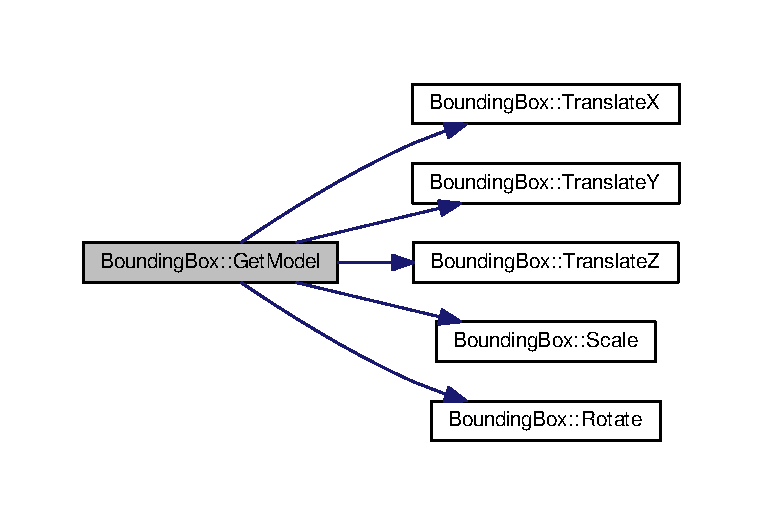
\includegraphics[width=350pt]{class_bounding_box_a5fd1769f7157e7df40a6ab6a242fcfcc_cgraph}
\end{center}
\end{figure}


\hypertarget{class_bounding_box_a6686a674cd3de57c987bccdfe6acbe92}{}\index{Bounding\+Box@{Bounding\+Box}!Get\+Rotate\+Bool@{Get\+Rotate\+Bool}}
\index{Get\+Rotate\+Bool@{Get\+Rotate\+Bool}!Bounding\+Box@{Bounding\+Box}}
\subsubsection[{Get\+Rotate\+Bool()}]{\setlength{\rightskip}{0pt plus 5cm}bool Bounding\+Box\+::\+Get\+Rotate\+Bool (
\begin{DoxyParamCaption}
{}
\end{DoxyParamCaption}
)}\label{class_bounding_box_a6686a674cd3de57c987bccdfe6acbe92}
Get\+Rotate\+Bools Returns the Get\+Rotate\+Bool bool to see if it is animated or not 
\begin{DoxyCode}
204                                 \{
205     \textcolor{keywordflow}{return} rotate\_bool;
206 \}
\end{DoxyCode}
\hypertarget{class_bounding_box_a262907e4b68e555edc57b21faef5685b}{}\index{Bounding\+Box@{Bounding\+Box}!Get\+Scale\+Bool@{Get\+Scale\+Bool}}
\index{Get\+Scale\+Bool@{Get\+Scale\+Bool}!Bounding\+Box@{Bounding\+Box}}
\subsubsection[{Get\+Scale\+Bool()}]{\setlength{\rightskip}{0pt plus 5cm}bool Bounding\+Box\+::\+Get\+Scale\+Bool (
\begin{DoxyParamCaption}
{}
\end{DoxyParamCaption}
)}\label{class_bounding_box_a262907e4b68e555edc57b21faef5685b}
Get\+Scale\+Bool Returns the scale\+\_\+bool bool to see if it is animated or not 
\begin{DoxyCode}
197                                \{
198     \textcolor{keywordflow}{return} scale\_bool;
199 \}
\end{DoxyCode}
\hypertarget{class_bounding_box_a501c1fd40b00ce6295fd60e1ed8cd92c}{}\index{Bounding\+Box@{Bounding\+Box}!Get\+Translate\+Bool@{Get\+Translate\+Bool}}
\index{Get\+Translate\+Bool@{Get\+Translate\+Bool}!Bounding\+Box@{Bounding\+Box}}
\subsubsection[{Get\+Translate\+Bool()}]{\setlength{\rightskip}{0pt plus 5cm}bool Bounding\+Box\+::\+Get\+Translate\+Bool (
\begin{DoxyParamCaption}
{}
\end{DoxyParamCaption}
)}\label{class_bounding_box_a501c1fd40b00ce6295fd60e1ed8cd92c}
Get\+Translate\+Bool Returns the translate\+\_\+bool bool to see if it is animated or not 
\begin{DoxyCode}
190                                    \{
191     \textcolor{keywordflow}{return} translate\_bool;
192 \}
\end{DoxyCode}
\hypertarget{class_bounding_box_a45332d45575fe93b516267436abcd4fe}{}\index{Bounding\+Box@{Bounding\+Box}!Get\+Translate\+To@{Get\+Translate\+To}}
\index{Get\+Translate\+To@{Get\+Translate\+To}!Bounding\+Box@{Bounding\+Box}}
\subsubsection[{Get\+Translate\+To()}]{\setlength{\rightskip}{0pt plus 5cm}glm\+::vec3 Bounding\+Box\+::\+Get\+Translate\+To (
\begin{DoxyParamCaption}
{}
\end{DoxyParamCaption}
)}\label{class_bounding_box_a45332d45575fe93b516267436abcd4fe}
Get\+Translate\+To Returns the Current position the \hyperlink{class_bounding_box}{Bounding\+Box} is at 
\begin{DoxyCode}
183                                     \{
184     \textcolor{keywordflow}{return} translateTo;
185 \}
\end{DoxyCode}
\hypertarget{class_bounding_box_a728a3700574a5d9fbcac6d94561336ed}{}\index{Bounding\+Box@{Bounding\+Box}!Rotate@{Rotate}}
\index{Rotate@{Rotate}!Bounding\+Box@{Bounding\+Box}}
\subsubsection[{Rotate(glm\+::vec3 rotate)}]{\setlength{\rightskip}{0pt plus 5cm}void Bounding\+Box\+::\+Rotate (
\begin{DoxyParamCaption}
\item[{glm\+::vec3}]{rotate\+To}
\end{DoxyParamCaption}
)}\label{class_bounding_box_a728a3700574a5d9fbcac6d94561336ed}
Rotate Method Controls the rotation of the asset 
\begin{DoxyCode}
120                                          \{
121         \textcolor{keywordflow}{if}(rotate.x <= 100.1f && rotate.y <= 100.1f && rotate.z <= 100.1f) \{
122                 rotate = rotate + glm::vec3(0.1f , 0.1f, 0.1f);
123         \}
124         \textcolor{keywordflow}{else} \{
125                 rotate = glm::vec3(0.1f, 0.1f, 0.1f);
126         \}
127 \}
\end{DoxyCode}


Here is the caller graph for this function\+:\nopagebreak
\begin{figure}[H]
\begin{center}
\leavevmode
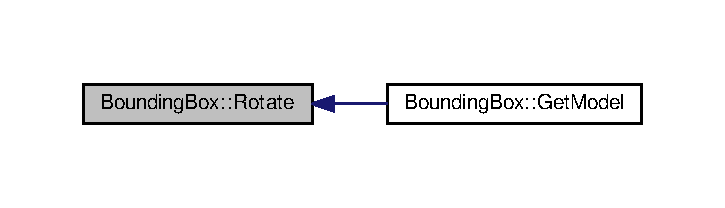
\includegraphics[width=348pt]{class_bounding_box_a728a3700574a5d9fbcac6d94561336ed_icgraph}
\end{center}
\end{figure}


\hypertarget{class_bounding_box_ab84e48c88a509b20a469ccf5e23c4f11}{}\index{Bounding\+Box@{Bounding\+Box}!Scale@{Scale}}
\index{Scale@{Scale}!Bounding\+Box@{Bounding\+Box}}
\subsubsection[{Scale(glm\+::vec3 scale)}]{\setlength{\rightskip}{0pt plus 5cm}void Bounding\+Box\+::\+Scale (
\begin{DoxyParamCaption}
\item[{glm\+::vec3}]{scale\+To}
\end{DoxyParamCaption}
)}\label{class_bounding_box_ab84e48c88a509b20a469ccf5e23c4f11}
Scale Method Controls the size of the Asset 
\begin{DoxyCode}
133                                        \{
134     \textcolor{keywordflow}{if}(scale.x < scaleTo.x && scale.y < scaleTo.y && scale.z < scaleTo.z) \{
135         scale = scale + glm::vec3(0.01f,0.01f,0.01f);
136     \}
137     \textcolor{keywordflow}{else} \{
138         scale = glm::vec3(1.0f,1.0f,1.0f);
139     \}
140 \}    
\end{DoxyCode}


Here is the caller graph for this function\+:\nopagebreak
\begin{figure}[H]
\begin{center}
\leavevmode
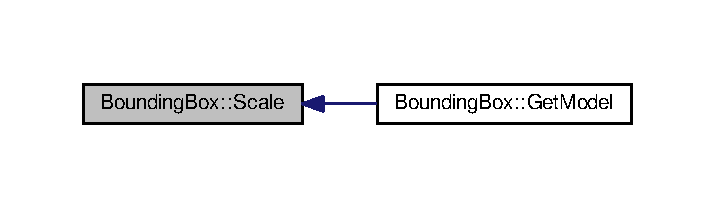
\includegraphics[width=343pt]{class_bounding_box_ab84e48c88a509b20a469ccf5e23c4f11_icgraph}
\end{center}
\end{figure}


\hypertarget{class_bounding_box_a9898275b1cd97761855156fc965412b1}{}\index{Bounding\+Box@{Bounding\+Box}!Translate\+X@{Translate\+X}}
\index{Translate\+X@{Translate\+X}!Bounding\+Box@{Bounding\+Box}}
\subsubsection[{Translate\+X()}]{\setlength{\rightskip}{0pt plus 5cm}void Bounding\+Box\+::\+Translate\+X (
\begin{DoxyParamCaption}
{}
\end{DoxyParamCaption}
)}\label{class_bounding_box_a9898275b1cd97761855156fc965412b1}
Translate Method This controls the translation animation, to move the assets on the x, y or z axis 
\begin{DoxyCode}
66                              \{
67                 \textcolor{keywordflow}{if}(translateTo.x < animateTo.x ) \{
68                         translateTo = translateTo + glm::vec3(0.1f,0.0f,0.0f);
69                         
70                         \textcolor{keywordflow}{if}(translateTo.x > animateTo.x)\{
71                                 translateTo = translateToSave;
72                         \}
73                 \}
74                 \textcolor{keywordflow}{else} \textcolor{keywordflow}{if}(translateTo.x > animateTo.x) \{
75                         translateTo = translateTo + glm::vec3(-0.1f,0.0f,0.0f);
76 
77                         \textcolor{keywordflow}{if}(translateTo.x < animateTo.x)\{
78                                 translateTo = translateToSave;
79                         \}
80                 \}
81 \}
\end{DoxyCode}


Here is the caller graph for this function\+:\nopagebreak
\begin{figure}[H]
\begin{center}
\leavevmode
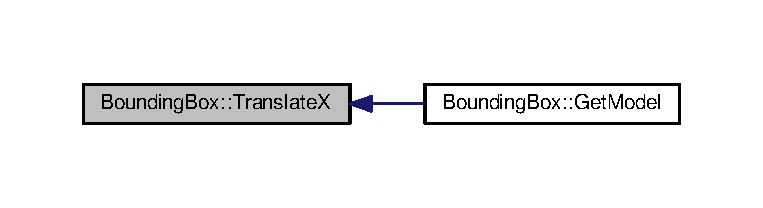
\includegraphics[width=350pt]{class_bounding_box_a9898275b1cd97761855156fc965412b1_icgraph}
\end{center}
\end{figure}


\hypertarget{class_bounding_box_aedff87fb2721b1e706e6e033e35b676b}{}\index{Bounding\+Box@{Bounding\+Box}!Translate\+Y@{Translate\+Y}}
\index{Translate\+Y@{Translate\+Y}!Bounding\+Box@{Bounding\+Box}}
\subsubsection[{Translate\+Y()}]{\setlength{\rightskip}{0pt plus 5cm}void Bounding\+Box\+::\+Translate\+Y (
\begin{DoxyParamCaption}
{}
\end{DoxyParamCaption}
)}\label{class_bounding_box_aedff87fb2721b1e706e6e033e35b676b}

\begin{DoxyCode}
83                              \{
84             \textcolor{keywordflow}{if}(translateTo.y < animateTo.y ) \{
85                        translateTo = translateTo + glm::vec3(0.0f,0.1f,0.0f);
86                        
87                        \textcolor{keywordflow}{if}(translateTo.y > animateTo.y)\{
88                                 translateTo = translateToSave;
89                        \}
90                 \}
91                 \textcolor{keywordflow}{else} \textcolor{keywordflow}{if}(translateTo.y > animateTo.y)\{
92                         translateTo = translateTo + glm::vec3(0.0f,-0.1f,0.0f);
93                   
94                         \textcolor{keywordflow}{if}(translateTo.y < animateTo.y)\{
95                                 translateTo = translateToSave;
96                         \}
97                 \}
98 \}
\end{DoxyCode}


Here is the caller graph for this function\+:\nopagebreak
\begin{figure}[H]
\begin{center}
\leavevmode
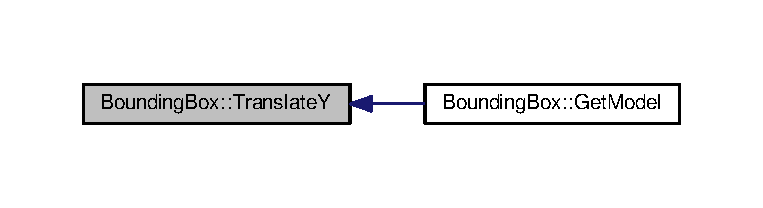
\includegraphics[width=350pt]{class_bounding_box_aedff87fb2721b1e706e6e033e35b676b_icgraph}
\end{center}
\end{figure}


\hypertarget{class_bounding_box_a33d133625c7a1a6f6dd7628f00388fd5}{}\index{Bounding\+Box@{Bounding\+Box}!Translate\+Z@{Translate\+Z}}
\index{Translate\+Z@{Translate\+Z}!Bounding\+Box@{Bounding\+Box}}
\subsubsection[{Translate\+Z()}]{\setlength{\rightskip}{0pt plus 5cm}void Bounding\+Box\+::\+Translate\+Z (
\begin{DoxyParamCaption}
{}
\end{DoxyParamCaption}
)}\label{class_bounding_box_a33d133625c7a1a6f6dd7628f00388fd5}

\begin{DoxyCode}
99                              \{
100                 \textcolor{keywordflow}{if}(translateTo.z < animateTo.z ) \{
101                         translateTo = translateTo + glm::vec3(0.0f,0.0f,0.1f);
102                         
103                         \textcolor{keywordflow}{if}(translateTo.z > animateTo.z)\{
104                                 translateTo = translateToSave;
105                         \}
106                 \}
107                 \textcolor{keywordflow}{else} \textcolor{keywordflow}{if}(translateTo.z > animateTo.z)\{
108                         translateTo = translateTo + glm::vec3(0.0f,0.0f,-0.1f);
109                         
110                         \textcolor{keywordflow}{if}(translateTo.z < animateTo.z)\{
111                                 translateTo = translateToSave;
112                         \}
113                 \}
114 \}
\end{DoxyCode}


Here is the caller graph for this function\+:\nopagebreak
\begin{figure}[H]
\begin{center}
\leavevmode
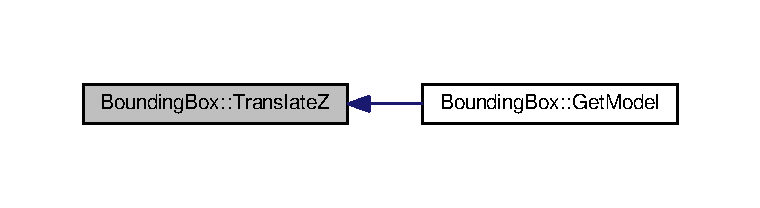
\includegraphics[width=350pt]{class_bounding_box_a33d133625c7a1a6f6dd7628f00388fd5_icgraph}
\end{center}
\end{figure}




The documentation for this class was generated from the following files\+:\begin{DoxyCompactItemize}
\item 
src/\hyperlink{_bounding_box_8h}{Bounding\+Box.\+h}\item 
src/\hyperlink{_bounding_box_8cc}{Bounding\+Box.\+cc}\end{DoxyCompactItemize}

\hypertarget{class_camera}{}\section{Camera Class Reference}
\label{class_camera}\index{Camera@{Camera}}


{\ttfamily \#include $<$Camera.\+h$>$}

\subsection*{Public Member Functions}
\begin{DoxyCompactItemize}
\item 
\hyperlink{class_camera_a01f94c3543f56ede7af49dc778f19331}{Camera} ()
\item 
glm\+::mat4 \hyperlink{class_camera_a37a2cb59aee3425a33672a6d5ae021f5}{Update\+Camera\+Position} (\hyperlink{common_8h_a0da83e35f29c11f7f3c637234f2149f9}{Control} control, int Mouse\+\_\+\+X, int Mouse\+\_\+\+Y)
\item 
void \hyperlink{class_camera_a985109173ffc496b53000c635aff5e06}{Collision\+Detection} (glm\+::vec3 B\+B\+\_\+\+Max, glm\+::vec3 B\+B\+\_\+\+Min)
\item 
glm\+::vec3 \hyperlink{class_camera_a948a60a6eb780a313ed59690bbaef811}{Get\+Camera\+Position} ()
\end{DoxyCompactItemize}


\subsection{Constructor \& Destructor Documentation}
\hypertarget{class_camera_a01f94c3543f56ede7af49dc778f19331}{}\index{Camera@{Camera}!Camera@{Camera}}
\index{Camera@{Camera}!Camera@{Camera}}
\subsubsection[{Camera()}]{\setlength{\rightskip}{0pt plus 5cm}Camera\+::\+Camera (
\begin{DoxyParamCaption}
{}
\end{DoxyParamCaption}
)}\label{class_camera_a01f94c3543f56ede7af49dc778f19331}
Controls calculations Controls all the movement and positions of the camera Uses keyboard and Mouse movements to move around the world space Tells the \hyperlink{class_camera}{Camera} matrix what position to look at and where to move 
\begin{DoxyCode}
10                \{
11           Camera\_Position = glm::vec3(0.0f, 0.5f, -10.0f);
12 
13       Camera\_Horizontal = 0.0f;
14       Camera\_Vertical = 0.0f;
15 
16           mouseDeltaX = 0.0;
17       mouseDeltaY = 0.0;
18 
19       Player\_Speed = 0.5; 
20 \}
\end{DoxyCode}


\subsection{Member Function Documentation}
\hypertarget{class_camera_a985109173ffc496b53000c635aff5e06}{}\index{Camera@{Camera}!Collision\+Detection@{Collision\+Detection}}
\index{Collision\+Detection@{Collision\+Detection}!Camera@{Camera}}
\subsubsection[{Collision\+Detection(glm\+::vec3 B\+B\+\_\+\+Max, glm\+::vec3 B\+B\+\_\+\+Min)}]{\setlength{\rightskip}{0pt plus 5cm}void Camera\+::\+Collision\+Detection (
\begin{DoxyParamCaption}
\item[{glm\+::vec3}]{B\+B\+\_\+\+Max, }
\item[{glm\+::vec3}]{B\+B\+\_\+\+Min}
\end{DoxyParamCaption}
)}\label{class_camera_a985109173ffc496b53000c635aff5e06}

\begin{DoxyCode}
114                                                               \{
115         Camera\_BB\_Max = Camera\_Position + glm::vec3(0.5f,0.5f,0.5f);
116         Camera\_BB\_Min = Camera\_Position + glm::vec3(-0.5f,-0.5f,-0.5f);
117  
118         \textcolor{keywordflow}{if} (BB\_Max.x > Camera\_BB\_Min.x && BB\_Min.x < Camera\_BB\_Max.x &&
119                 BB\_Max.y > Camera\_BB\_Min.y && BB\_Min.y < Camera\_BB\_Max.y &&
120                 BB\_Max.z > Camera\_BB\_Min.z && BB\_Min.z < Camera\_BB\_Max.z) \{
121             cout << \textcolor{stringliteral}{"Camera Collision!"} << endl;
122             
123             \textcolor{keywordflow}{if}( ControlSave == \textcolor{stringliteral}{"UP"} ) \{
124                     Camera\_Position -=  Movement\_Z * Player\_Speed;     
125             \}
126                 \textcolor{keywordflow}{else} \textcolor{keywordflow}{if}( ControlSave == \textcolor{stringliteral}{"DOWN"} ) \{
127                 Camera\_Position += Movement\_Z * Player\_Speed;
128             \} 
129                 \textcolor{keywordflow}{else} \textcolor{keywordflow}{if}( ControlSave == \textcolor{stringliteral}{"LEFT"} ) \{
130                 Camera\_Position += Movement\_X * Player\_Speed;
131             \} 
132                 \textcolor{keywordflow}{else} \textcolor{keywordflow}{if}( ControlSave == \textcolor{stringliteral}{"RIGHT"} ) \{
133                 Camera\_Position -= Movement\_X * Player\_Speed;
134             \}
135                 \textcolor{keywordflow}{else} \textcolor{keywordflow}{if}( ControlSave == \textcolor{stringliteral}{"JUMP"} ) \{
136                         Camera\_Position.y -= 0.5f * Player\_Speed;
137                 \}
138                 \textcolor{keywordflow}{else} \textcolor{keywordflow}{if}( ControlSave == \textcolor{stringliteral}{"CROUCH"} ) \{
139                         Camera\_Position.y += 0.5f * Player\_Speed;
140                 \}
141         \}
142 \}
\end{DoxyCode}
\hypertarget{class_camera_a948a60a6eb780a313ed59690bbaef811}{}\index{Camera@{Camera}!Get\+Camera\+Position@{Get\+Camera\+Position}}
\index{Get\+Camera\+Position@{Get\+Camera\+Position}!Camera@{Camera}}
\subsubsection[{Get\+Camera\+Position()}]{\setlength{\rightskip}{0pt plus 5cm}glm\+::vec3 Camera\+::\+Get\+Camera\+Position (
\begin{DoxyParamCaption}
{}
\end{DoxyParamCaption}
)}\label{class_camera_a948a60a6eb780a313ed59690bbaef811}
\hypertarget{class_camera_a37a2cb59aee3425a33672a6d5ae021f5}{}\index{Camera@{Camera}!Update\+Camera\+Position@{Update\+Camera\+Position}}
\index{Update\+Camera\+Position@{Update\+Camera\+Position}!Camera@{Camera}}
\subsubsection[{Update\+Camera\+Position(\+Control control, int Mouse\+\_\+\+X, int Mouse\+\_\+\+Y)}]{\setlength{\rightskip}{0pt plus 5cm}glm\+::mat4 Camera\+::\+Update\+Camera\+Position (
\begin{DoxyParamCaption}
\item[{{\bf Control}}]{control, }
\item[{int}]{Mouse\+\_\+\+X, }
\item[{int}]{Mouse\+\_\+\+Y}
\end{DoxyParamCaption}
)}\label{class_camera_a37a2cb59aee3425a33672a6d5ae021f5}
Drawing the world. Draws the assets to the world by calling \hyperlink{class_game_asset_manager}{Game\+Asset\+Manager} Sends the camera positions and movements to the translate shader \hyperlink{class_camera}{Camera} Direction Calculates the distance each camera movement changes the camera direction

Keyboard Input Use This gets the Current Control State and then calculates the appropriate changes to the \hyperlink{class_camera}{Camera} Position.

\hyperlink{class_camera}{Camera} view matrix. changes where the camera position looks up to use the camera position changes the direction you look at Makes the world the correct orientation
\begin{DoxyCode}
27                                                                               \{
32         \textcolor{comment}{// mouse delta position inverted}
33     mouseDeltaX = -Mouse\_X;
34     mouseDeltaY = -Mouse\_Y;
35 
36         Camera\_Horizontal += 0.001f * mouseDeltaX;
37 
38         \textcolor{keywordflow}{if}((Camera\_Vertical + (0.01f * mouseDeltaY)) < 3.0f && (Camera\_Vertical + (0.01f * mouseDeltaY)) > 
      -3.0f )\{
39             Camera\_Vertical += 0.001f * mouseDeltaY;
40         \}
41 
42         glm::vec3 direction(
43         cos(Camera\_Vertical) * sin(Camera\_Horizontal),
44         sin(Camera\_Vertical),
45         cos(Camera\_Vertical) * cos(Camera\_Horizontal)
46     );
47     
48         glm::vec3 Walk\_direction(
49         cos(Camera\_Vertical) * sin(Camera\_Horizontal),
50         0,
51         cos(Camera\_Vertical) * cos(Camera\_Horizontal)
52     );
53         
54     Movement\_Z = Walk\_direction;
55 
56     Movement\_X = glm::vec3(
57         sin(Camera\_Horizontal - 3.14f/2.0f),
58         0,
59         cos(Camera\_Horizontal - 3.14f/2.0f)
60     );
61 
62     glm::vec3 vup = glm::cross(Movement\_X, Movement\_Z);
63         
69         \textcolor{keywordflow}{if}(control == \hyperlink{common_8h_a0da83e35f29c11f7f3c637234f2149f9aba595d8bca8bc5e67c37c0a9d89becfa}{UP}) \{
70         Camera\_Position +=  Movement\_Z * Player\_Speed;
71         ControlSave = \textcolor{stringliteral}{"UP"};
72     \}
73         \textcolor{keywordflow}{else} \textcolor{keywordflow}{if}(control == \hyperlink{common_8h_a0da83e35f29c11f7f3c637234f2149f9a9b0b4a95b99523966e0e34ffdadac9da}{DOWN}) \{
74         Camera\_Position -= Movement\_Z * Player\_Speed;
75         ControlSave = \textcolor{stringliteral}{"DOWN"};
76     \} 
77         \textcolor{keywordflow}{else} \textcolor{keywordflow}{if}(control == \hyperlink{common_8h_a0da83e35f29c11f7f3c637234f2149f9adb45120aafd37a973140edee24708065}{LEFT}) \{
78         Camera\_Position -= Movement\_X * Player\_Speed;
79         ControlSave = \textcolor{stringliteral}{"LEFT"};
80     \} 
81         \textcolor{keywordflow}{else} \textcolor{keywordflow}{if}(control == \hyperlink{common_8h_a0da83e35f29c11f7f3c637234f2149f9aec8379af7490bb9eaaf579cf17876f38}{RIGHT}) \{
82         Camera\_Position += Movement\_X * Player\_Speed;
83         ControlSave = \textcolor{stringliteral}{"RIGHT"};
84     \}
85         \textcolor{keywordflow}{else} \textcolor{keywordflow}{if}(control == \hyperlink{common_8h_a0da83e35f29c11f7f3c637234f2149f9a1f28d4392b1c1e7da2af2283632d81e1}{JUMP}) \{
86                 Camera\_Position.y += 0.5f * Player\_Speed;
87                 ControlSave = \textcolor{stringliteral}{"JUMP"};
88         \}
89         \textcolor{keywordflow}{else} \textcolor{keywordflow}{if}(control == \hyperlink{common_8h_a0da83e35f29c11f7f3c637234f2149f9a3cdd4783c5dbeae45bbcd15570a6b273}{CROUCH}) \{
90                 Camera\_Position.y -= 0.5f * Player\_Speed;
91                 ControlSave = \textcolor{stringliteral}{"CROUCH"};
92         \}
93         \textcolor{keywordflow}{else} \textcolor{keywordflow}{if}(control == \hyperlink{common_8h_a0da83e35f29c11f7f3c637234f2149f9ab107229d44d042caa8ab8df4c8acaa1f}{PRINT}) \{
94                 cout << \textcolor{stringliteral}{"********************************************************************"} << endl;
95                 cout << \textcolor{stringliteral}{"Camera Position: "} << glm::to\_string(Camera\_Position) << endl;
96                 \textcolor{comment}{//cout << "Camera Old Position: " << glm::to\_string(Camera\_Old\_Position) << endl;}
97                 
98                 cout << \textcolor{stringliteral}{"Camera Axis Alligned Bounding Box"} << endl;
99                 cout << \textcolor{stringliteral}{"********************************************************************"} << endl;
100         \}
101         \textcolor{comment}{//cout << "Camera\_Position" << glm::to\_string(Camera\_Position) <<endl;}
108 \textcolor{comment}{}        \textcolor{keywordflow}{return} glm::lookAt(Camera\_Position, 
109                            Camera\_Position + direction, 
110                            vup);
111    
112 \}
\end{DoxyCode}


The documentation for this class was generated from the following files\+:\begin{DoxyCompactItemize}
\item 
src/\hyperlink{_camera_8h}{Camera.\+h}\item 
src/\hyperlink{_camera_8cc}{Camera.\+cc}\end{DoxyCompactItemize}

\hypertarget{class_cube_asset}{}\section{Cube\+Asset Class Reference}
\label{class_cube_asset}\index{Cube\+Asset@{Cube\+Asset}}


{\ttfamily \#include $<$Cube\+Asset.\+h$>$}



Inheritance diagram for Cube\+Asset\+:\nopagebreak
\begin{figure}[H]
\begin{center}
\leavevmode
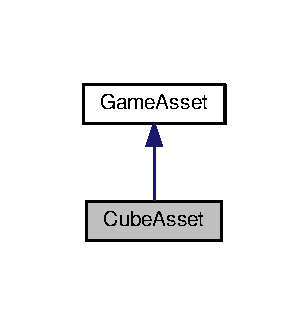
\includegraphics[width=148pt]{class_cube_asset__inherit__graph}
\end{center}
\end{figure}


Collaboration diagram for Cube\+Asset\+:\nopagebreak
\begin{figure}[H]
\begin{center}
\leavevmode
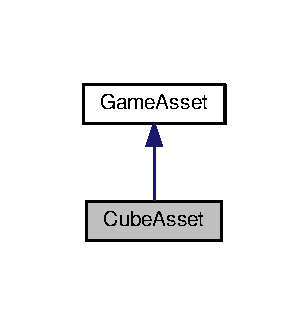
\includegraphics[width=148pt]{class_cube_asset__coll__graph}
\end{center}
\end{figure}
\subsection*{Public Member Functions}
\begin{DoxyCompactItemize}
\item 
\hyperlink{class_cube_asset_a77f29d64dc1ed34067948d73302a4d4f}{Cube\+Asset} (glm\+::vec3 xyz\+Position, glm\+::vec3 translate\+To, glm\+::vec3 animate\+To, bool translate\+\_\+bool, glm\+::vec3 rotate, bool rotate\+\_\+bool, glm\+::vec3 scale, bool scale\+\_\+bool, string Asset\+Type)
\item 
\hyperlink{class_cube_asset_ab3ab9a5da82cbf8537a28652410093b1}{$\sim$\+Cube\+Asset} ()
\item 
void \hyperlink{class_cube_asset_a1af568486056e254ffcf98fd99947bfe}{Draw} (G\+Luint)
\end{DoxyCompactItemize}


\subsection{Constructor \& Destructor Documentation}
\hypertarget{class_cube_asset_a77f29d64dc1ed34067948d73302a4d4f}{}\index{Cube\+Asset@{Cube\+Asset}!Cube\+Asset@{Cube\+Asset}}
\index{Cube\+Asset@{Cube\+Asset}!Cube\+Asset@{Cube\+Asset}}
\subsubsection[{Cube\+Asset(glm\+::vec3 xyz\+Position, glm\+::vec3 translate\+To, glm\+::vec3 animate\+To, bool translate\+\_\+bool, glm\+::vec3 rotate, bool rotate\+\_\+bool, glm\+::vec3 scale, bool scale\+\_\+bool, string Asset\+Type)}]{\setlength{\rightskip}{0pt plus 5cm}Cube\+Asset\+::\+Cube\+Asset (
\begin{DoxyParamCaption}
\item[{glm\+::vec3}]{xyz\+Position, }
\item[{glm\+::vec3}]{translate\+To, }
\item[{glm\+::vec3}]{animate\+To, }
\item[{bool}]{translate\+\_\+bool, }
\item[{glm\+::vec3}]{rotate, }
\item[{bool}]{rotate\+\_\+bool, }
\item[{glm\+::vec3}]{scale, }
\item[{bool}]{scale\+\_\+bool, }
\item[{string}]{Asset\+Type}
\end{DoxyParamCaption}
)}\label{class_cube_asset_a77f29d64dc1ed34067948d73302a4d4f}
model coordinates, origin at centre. Sets cordinates to a cube with the center point 0.\+0 but moved to where the x, y, z variables calls them from the gameworld class through the G\+Lfloat x,y,z variables.

Color Buffer. Colour of Cube Asset Saddle Brown Uses R\+G\+B values to set the colour.

Element buffer. Draws the cube voxel up of 12 Triangles Two Triangles per Face.
\begin{DoxyCode}
7 : \hyperlink{class_game_asset_a9de932075d9b4263e7fb24fbfd163a61}{GameAsset}(xyzPosition, translateTo, animateTo, translate\_bool, rotate, rotate\_bool, scale, 
      scale\_bool, AssetType) \{
8 
9   Position = xyzPosition;
16   GLfloat vertex\_buffer[]\{
17       0.5f + xyzPosition.x  , 0.5f + xyzPosition.y  , -0.5f + xyzPosition.z
18     , 0.5f + xyzPosition.x  ,-0.5f + xyzPosition.y  , -0.5f + xyzPosition.z
19     ,-0.5f + xyzPosition.x  , 0.5f + xyzPosition.y  , -0.5f + xyzPosition.z
20     ,-0.5f + xyzPosition.x  ,-0.5f + xyzPosition.y  , -0.5f + xyzPosition.z
21     , 0.5f + xyzPosition.x  , 0.5f + xyzPosition.y  ,  0.5f + xyzPosition.z 
22     , 0.5f + xyzPosition.x  ,-0.5f + xyzPosition.y  ,  0.5f + xyzPosition.z
23     ,-0.5f + xyzPosition.x  , 0.5f + xyzPosition.y  ,  0.5f + xyzPosition.z
24     ,-0.5f + xyzPosition.x  ,-0.5f + xyzPosition.y  ,  0.5f + xyzPosition.z
25   \};
26 
27   GLfloat vertex\_buffer\_length = \textcolor{keyword}{sizeof}(vertex\_buffer);
28 
34   GLfloat colour\_buffer[] = \{
35 
36      0.139f, 0.069f, 0.019f,
37      0.139f, 0.069f, 0.019f,
38      0.139f, 0.069f, 0.019f,
39      0.139f, 0.069f, 0.019f,
40      0.139f, 0.069f, 0.019f,
41      0.139f, 0.069f, 0.019f,
42      0.139f, 0.069f, 0.019f,
43      0.139f, 0.069f, 0.019f
44   \};
45   colour\_buffer\_length = \textcolor{keyword}{sizeof}(colour\_buffer);
51   GLuint element\_buffer []  \{
52       0, 1, 2   
53     , 1, 3, 2
54     , 0, 4, 1   
55     , 1, 5, 4   
56     , 5, 7, 4   
57     , 7, 6, 4   
58     , 3, 7, 6   
59     , 2, 3, 6   
60     , 1, 5, 7   
61     , 1, 3, 7   
62     , 0, 4, 6   
63     , 0, 2, 6   
64   \};
65   element\_buffer\_length = \textcolor{keyword}{sizeof}(element\_buffer);
66 
67   \textcolor{comment}{// Transfer buffers to the GPU}
68 
69   \textcolor{comment}{// create buffer}
70   glGenBuffers(1, &vertex\_buffer\_token);
71   \textcolor{comment}{// immediately bind the buffer and transfer the data}
72   glBindBuffer(GL\_ARRAY\_BUFFER, vertex\_buffer\_token);
73   glBufferData(GL\_ARRAY\_BUFFER, vertex\_buffer\_length, vertex\_buffer, GL\_STATIC\_DRAW);
74   
75   \textcolor{comment}{// Binds the buffer to transfer the data}
76   glGenBuffers(1, &colour\_buffer\_token);
77   glBindBuffer(GL\_ARRAY\_BUFFER, colour\_buffer\_token);
78   glBufferData(GL\_ARRAY\_BUFFER, colour\_buffer\_length, colour\_buffer, GL\_STATIC\_DRAW);
79 
80 
81   glGenBuffers(1, &element\_buffer\_token);
82   glBindBuffer(GL\_ELEMENT\_ARRAY\_BUFFER, element\_buffer\_token);
83   glBufferData(GL\_ELEMENT\_ARRAY\_BUFFER, element\_buffer\_length, element\_buffer, GL\_STATIC\_DRAW);
84 \}
\end{DoxyCode}
\hypertarget{class_cube_asset_ab3ab9a5da82cbf8537a28652410093b1}{}\index{Cube\+Asset@{Cube\+Asset}!````~Cube\+Asset@{$\sim$\+Cube\+Asset}}
\index{````~Cube\+Asset@{$\sim$\+Cube\+Asset}!Cube\+Asset@{Cube\+Asset}}
\subsubsection[{$\sim$\+Cube\+Asset()}]{\setlength{\rightskip}{0pt plus 5cm}Cube\+Asset\+::$\sim$\+Cube\+Asset (
\begin{DoxyParamCaption}
{}
\end{DoxyParamCaption}
)}\label{class_cube_asset_ab3ab9a5da82cbf8537a28652410093b1}

\begin{DoxyCode}
87                       \{
88 \}
\end{DoxyCode}


\subsection{Member Function Documentation}
\hypertarget{class_cube_asset_a1af568486056e254ffcf98fd99947bfe}{}\index{Cube\+Asset@{Cube\+Asset}!Draw@{Draw}}
\index{Draw@{Draw}!Cube\+Asset@{Cube\+Asset}}
\subsubsection[{Draw(\+G\+Luint)}]{\setlength{\rightskip}{0pt plus 5cm}void Cube\+Asset\+::\+Draw (
\begin{DoxyParamCaption}
\item[{G\+Luint}]{program\+\_\+token}
\end{DoxyParamCaption}
)\hspace{0.3cm}{\ttfamily [virtual]}}\label{class_cube_asset_a1af568486056e254ffcf98fd99947bfe}
use the previously transferred buffer as the vertex array. This way we transfer the buffer once -- at construction -- not on every frame.

Uses the Previously transferred buffer as the color array. This way We transfer the buffer once -- at constuction -- not on every frame

Implements \hyperlink{class_game_asset_a961aa51ca0a9961fc584c0b5d5431300}{Game\+Asset}.


\begin{DoxyCode}
97                                          \{
98   \textcolor{keywordflow}{if}(!glIsProgram(program\_token)) \{
99     \textcolor{comment}{//cerr << "Drawing Cube with invalid program" << endl;}
100     \textcolor{keywordflow}{return};
101   \}
102   GLint validation\_ok;
103   glValidateProgram(program\_token);
104   glGetProgramiv(program\_token, GL\_VALIDATE\_STATUS, &validation\_ok);
105   \textcolor{keywordflow}{if}(!validation\_ok) \{
106     GLint maxLength = 0;
107     glGetProgramiv(program\_token, GL\_INFO\_LOG\_LENGTH, &maxLength);
108 
109     \textcolor{comment}{// The maxLength includes the NULL character}
110     std::vector<char> errorLog(maxLength);
111     glGetProgramInfoLog(program\_token, maxLength, &maxLength, &errorLog[0]);
112 
113     std::cerr << \textcolor{stringliteral}{"Invalid program "} << program\_token << \textcolor{stringliteral}{" with error code "} << validation\_ok << std::endl;
114     \textcolor{keywordflow}{for}(\textcolor{keyword}{auto} c: errorLog) \{
115       std::cerr << c;
116     \}
117     exit(-1);
118   \}
119 
120   GLuint position\_attrib = glGetAttribLocation(program\_token, \textcolor{stringliteral}{"position"});
121   \hyperlink{_cube_asset_8cc_a75f201b0e53e68726854997957322b8d}{checkGLError}();
122 
123   glUseProgram(program\_token);
124   \hyperlink{_cube_asset_8cc_a75f201b0e53e68726854997957322b8d}{checkGLError}();
129   glEnableVertexAttribArray(0);
130   glBindBuffer(GL\_ARRAY\_BUFFER, vertex\_buffer\_token);
131   glVertexAttribPointer(
132     position\_attrib,        \textcolor{comment}{/* attribute */}
133     3,        \textcolor{comment}{/* size */}
134     GL\_FLOAT,   \textcolor{comment}{/* type */}
135     GL\_FALSE,   \textcolor{comment}{/* normalized? */}
136     0,        \textcolor{comment}{/* stride */}
137     (\textcolor{keywordtype}{void}*)0    \textcolor{comment}{/* array buffer offset */}
138   );
139   glEnableVertexAttribArray(1);
140   \hyperlink{_cube_asset_8cc_a75f201b0e53e68726854997957322b8d}{checkGLError}();
145   glBindBuffer(GL\_ARRAY\_BUFFER, colour\_buffer\_token);
146   glVertexAttribPointer(
147     1,        \textcolor{comment}{/* attribute */}
148     3,        \textcolor{comment}{/* size */}
149     GL\_FLOAT,   \textcolor{comment}{/* type */}
150     GL\_FALSE,   \textcolor{comment}{/* normalized? */}
151     0,        \textcolor{comment}{/* stride */}
152     (\textcolor{keywordtype}{void}*)0    \textcolor{comment}{/* array buffer offset */}
153   );
154   \hyperlink{_cube_asset_8cc_a75f201b0e53e68726854997957322b8d}{checkGLError}();
155 
156   glBindBuffer(GL\_ELEMENT\_ARRAY\_BUFFER, element\_buffer\_token);
157   glDrawElements(
158     GL\_TRIANGLES,
159     element\_buffer\_length,
160     GL\_UNSIGNED\_INT,
161     (GLvoid*) 0
162   );
163   \hyperlink{_cube_asset_8cc_a75f201b0e53e68726854997957322b8d}{checkGLError}();
164 
165   glDisableVertexAttribArray(position\_attrib);
166 \}
\end{DoxyCode}


The documentation for this class was generated from the following files\+:\begin{DoxyCompactItemize}
\item 
src/\hyperlink{_cube_asset_8h}{Cube\+Asset.\+h}\item 
src/\hyperlink{_cube_asset_8cc}{Cube\+Asset.\+cc}\end{DoxyCompactItemize}

\hypertarget{class_diamond_asset}{}\section{Diamond\+Asset Class Reference}
\label{class_diamond_asset}\index{Diamond\+Asset@{Diamond\+Asset}}


{\ttfamily \#include $<$Diamond\+Asset.\+h$>$}



Inheritance diagram for Diamond\+Asset\+:\nopagebreak
\begin{figure}[H]
\begin{center}
\leavevmode
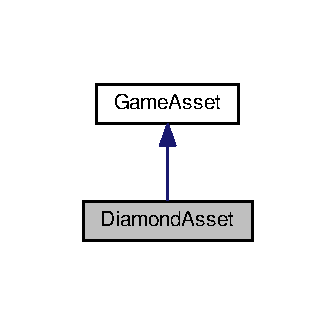
\includegraphics[width=161pt]{class_diamond_asset__inherit__graph}
\end{center}
\end{figure}


Collaboration diagram for Diamond\+Asset\+:\nopagebreak
\begin{figure}[H]
\begin{center}
\leavevmode
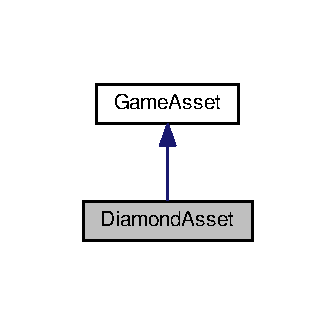
\includegraphics[width=161pt]{class_diamond_asset__coll__graph}
\end{center}
\end{figure}
\subsection*{Public Member Functions}
\begin{DoxyCompactItemize}
\item 
\hyperlink{class_diamond_asset_a297efbf3312ce0efba79f055a076481c}{Diamond\+Asset} (glm\+::vec3 xyz\+Position, glm\+::vec3 translate\+To, glm\+::vec3 animate\+To, bool translate\+\_\+bool, glm\+::vec3 rotate, bool rotate\+\_\+bool, glm\+::vec3 scale, bool scale\+\_\+bool, string Asset\+Type)
\item 
\hyperlink{class_diamond_asset_a1b7bf6ba76651a9304943f2c41fe36b8}{$\sim$\+Diamond\+Asset} ()
\item 
void \hyperlink{class_diamond_asset_a0c259031894623285b3b511321c73abb}{Draw} (G\+Luint)
\end{DoxyCompactItemize}


\subsection{Constructor \& Destructor Documentation}
\hypertarget{class_diamond_asset_a297efbf3312ce0efba79f055a076481c}{}\index{Diamond\+Asset@{Diamond\+Asset}!Diamond\+Asset@{Diamond\+Asset}}
\index{Diamond\+Asset@{Diamond\+Asset}!Diamond\+Asset@{Diamond\+Asset}}
\subsubsection[{Diamond\+Asset(glm\+::vec3 xyz\+Position, glm\+::vec3 translate\+To, glm\+::vec3 animate\+To, bool translate\+\_\+bool, glm\+::vec3 rotate, bool rotate\+\_\+bool, glm\+::vec3 scale, bool scale\+\_\+bool, string Asset\+Type)}]{\setlength{\rightskip}{0pt plus 5cm}Diamond\+Asset\+::\+Diamond\+Asset (
\begin{DoxyParamCaption}
\item[{glm\+::vec3}]{xyz\+Position, }
\item[{glm\+::vec3}]{translate\+To, }
\item[{glm\+::vec3}]{animate\+To, }
\item[{bool}]{translate\+\_\+bool, }
\item[{glm\+::vec3}]{rotate, }
\item[{bool}]{rotate\+\_\+bool, }
\item[{glm\+::vec3}]{scale, }
\item[{bool}]{scale\+\_\+bool, }
\item[{string}]{Asset\+Type}
\end{DoxyParamCaption}
)}\label{class_diamond_asset_a297efbf3312ce0efba79f055a076481c}
model coordinates, origin at centre. Sets cordinates to a Diamond with the center point 0.\+0 but moved to where the x, y, z variables calls them from the gameworld class through the G\+Lfloat x,y,z variables.

Color Buffer. Colour of Cube Asset Red Uses R\+G\+B values to set the colour.

Element buffer. Draws the Diamond up of 8 Triangles One Triangles per Face
\begin{DoxyCode}
7 : \hyperlink{class_game_asset_a9de932075d9b4263e7fb24fbfd163a61}{GameAsset}(xyzPosition, translateTo, animateTo, translate\_bool, rotate, rotate\_bool, scale, 
      scale\_bool, AssetType) \{
8 
15   GLfloat vertex\_buffer [] \{
16      -0.5f + xyzPosition.x  , 0.0f + xyzPosition.y   , 0.0f + xyzPosition.z
17      ,0.5f + xyzPosition.x  , 0.0f + xyzPosition.y   , 0.0f + xyzPosition.z
18      ,0.0f + xyzPosition.x  ,-0.5f + xyzPosition.y   , 0.0f + xyzPosition.z
19      ,0.0f + xyzPosition.x  , 0.5f + xyzPosition.y   , 0.0f + xyzPosition.z
20      ,0.0f + xyzPosition.x  , 0.0f + xyzPosition.y   ,-0.5f + xyzPosition.z
21      ,0.0f + xyzPosition.x  , 0.0f + xyzPosition.y   , 0.5f + xyzPosition.z
22   \};
23   GLfloat vertex\_buffer\_length = \textcolor{keyword}{sizeof}(vertex\_buffer);
29   GLfloat colour\_buffer[] = \{
30 
31      1.000f, 0.000f, 0.000f,
32      1.000f, 0.000f, 0.000f,
33      1.000f, 0.000f, 0.000f,
34      1.000f, 0.000f, 0.000f,
35      1.000f, 0.000f, 0.000f,
36      1.000f, 0.000f, 0.000f
37   \};
38   colour\_buffer\_length = \textcolor{keyword}{sizeof}(colour\_buffer);
44   GLuint element\_buffer []  \{
45       0, 3, 5   
46     , 3, 1, 5
47     , 0, 5, 2   
48     , 5, 1, 2
49     , 0, 3, 4
50     , 3, 1, 4
51     , 0, 4, 2
52     , 4, 1, 2
53   \};
54   element\_buffer\_length = \textcolor{keyword}{sizeof}(element\_buffer);
55 
56 
57 
58   \textcolor{comment}{// Transfer buffers to the GPU}
59 
60   \textcolor{comment}{// create buffer}
61   glGenBuffers(1, &vertex\_buffer\_token);
62   \textcolor{comment}{// immediately bind the buffer and transfer the data}
63   glBindBuffer(GL\_ARRAY\_BUFFER, vertex\_buffer\_token);
64   glBufferData(GL\_ARRAY\_BUFFER, vertex\_buffer\_length, vertex\_buffer, GL\_STATIC\_DRAW);
65 
66   \textcolor{comment}{// Binds the buffer and transfers the data}
67   glGenBuffers(1, &colour\_buffer\_token);
68   glBindBuffer(GL\_ARRAY\_BUFFER, colour\_buffer\_token);
69   glBufferData(GL\_ARRAY\_BUFFER, colour\_buffer\_length, colour\_buffer, GL\_STATIC\_DRAW);
70 
71 
72   glGenBuffers(1, &element\_buffer\_token);
73   glBindBuffer(GL\_ELEMENT\_ARRAY\_BUFFER, element\_buffer\_token);
74   glBufferData(GL\_ELEMENT\_ARRAY\_BUFFER, element\_buffer\_length, element\_buffer, GL\_STATIC\_DRAW);
75 \}
\end{DoxyCode}
\hypertarget{class_diamond_asset_a1b7bf6ba76651a9304943f2c41fe36b8}{}\index{Diamond\+Asset@{Diamond\+Asset}!````~Diamond\+Asset@{$\sim$\+Diamond\+Asset}}
\index{````~Diamond\+Asset@{$\sim$\+Diamond\+Asset}!Diamond\+Asset@{Diamond\+Asset}}
\subsubsection[{$\sim$\+Diamond\+Asset()}]{\setlength{\rightskip}{0pt plus 5cm}Diamond\+Asset\+::$\sim$\+Diamond\+Asset (
\begin{DoxyParamCaption}
{}
\end{DoxyParamCaption}
)}\label{class_diamond_asset_a1b7bf6ba76651a9304943f2c41fe36b8}

\begin{DoxyCode}
77                             \{
78 \}
\end{DoxyCode}


\subsection{Member Function Documentation}
\hypertarget{class_diamond_asset_a0c259031894623285b3b511321c73abb}{}\index{Diamond\+Asset@{Diamond\+Asset}!Draw@{Draw}}
\index{Draw@{Draw}!Diamond\+Asset@{Diamond\+Asset}}
\subsubsection[{Draw(\+G\+Luint)}]{\setlength{\rightskip}{0pt plus 5cm}void Diamond\+Asset\+::\+Draw (
\begin{DoxyParamCaption}
\item[{G\+Luint}]{program\+\_\+token}
\end{DoxyParamCaption}
)\hspace{0.3cm}{\ttfamily [virtual]}}\label{class_diamond_asset_a0c259031894623285b3b511321c73abb}
use the previously transferred buffer as the vertex array. This way we transfer the buffer once -- at construction -- not on every frame.

Uses the Previously transferred buffer as the color array. This way We transfer the buffer once -- at constuction -- not on every frame

Implements \hyperlink{class_game_asset_a961aa51ca0a9961fc584c0b5d5431300}{Game\+Asset}.


\begin{DoxyCode}
87                                             \{
88   \textcolor{keywordflow}{if}(!glIsProgram(program\_token)) \{
89     \textcolor{comment}{//std::cerr << "Drawing Diamond with invalid program" << std::endl;}
90     \textcolor{keywordflow}{return};
91   \}
92   GLint validation\_ok;
93   glValidateProgram(program\_token);
94   glGetProgramiv(program\_token, GL\_VALIDATE\_STATUS, &validation\_ok);
95   \textcolor{keywordflow}{if}(!validation\_ok) \{
96     GLint maxLength = 0;
97     glGetProgramiv(program\_token, GL\_INFO\_LOG\_LENGTH, &maxLength);
98 
99     \textcolor{comment}{// The maxLength includes the NULL character}
100     std::vector<char> errorLog(maxLength);
101     glGetProgramInfoLog(program\_token, maxLength, &maxLength, &errorLog[0]);
102 
103     std::cerr << \textcolor{stringliteral}{"Invalid program "} << program\_token << \textcolor{stringliteral}{" with error code "} << validation\_ok << std::endl;
104     \textcolor{keywordflow}{for}(\textcolor{keyword}{auto} c: errorLog) \{
105       std::cerr << c;
106     \}
107     exit(-1);
108   \}
109 
110   GLuint position\_attrib = glGetAttribLocation(program\_token, \textcolor{stringliteral}{"position"});
111   \hyperlink{_diamond_asset_8cc_a75f201b0e53e68726854997957322b8d}{checkGLError}();
112 
113   glUseProgram(program\_token);
114   \hyperlink{_diamond_asset_8cc_a75f201b0e53e68726854997957322b8d}{checkGLError}();
119   glEnableVertexAttribArray(0);
120   glBindBuffer(GL\_ARRAY\_BUFFER, vertex\_buffer\_token);
121   glVertexAttribPointer(
122     position\_attrib,        \textcolor{comment}{/* attribute */}
123     3,        \textcolor{comment}{/* size */}
124     GL\_FLOAT,   \textcolor{comment}{/* type */}
125     GL\_FALSE,   \textcolor{comment}{/* normalized? */}
126     0,        \textcolor{comment}{/* stride */}
127     (\textcolor{keywordtype}{void}*)0    \textcolor{comment}{/* array buffer offset */}
128   );
129   glEnableVertexAttribArray(1);
130   \hyperlink{_diamond_asset_8cc_a75f201b0e53e68726854997957322b8d}{checkGLError}();
135   glBindBuffer(GL\_ARRAY\_BUFFER, colour\_buffer\_token);
136   glVertexAttribPointer(
137     1,        \textcolor{comment}{/* attribute */}
138     3,        \textcolor{comment}{/* size */}
139     GL\_FLOAT,   \textcolor{comment}{/* type */}
140     GL\_FALSE,   \textcolor{comment}{/* normalized? */}
141     0,        \textcolor{comment}{/* stride */}
142     (\textcolor{keywordtype}{void}*)0    \textcolor{comment}{/* array buffer offset */}
143   );
144   \hyperlink{_diamond_asset_8cc_a75f201b0e53e68726854997957322b8d}{checkGLError}();
145 
146   glBindBuffer(GL\_ELEMENT\_ARRAY\_BUFFER, element\_buffer\_token);
147   glDrawElements(
148     GL\_TRIANGLES,
149     element\_buffer\_length,
150     GL\_UNSIGNED\_INT,
151     (GLvoid*) 0
152   );
153   \hyperlink{_diamond_asset_8cc_a75f201b0e53e68726854997957322b8d}{checkGLError}();
154 
155   glDisableVertexAttribArray(position\_attrib);
156 \}
\end{DoxyCode}


The documentation for this class was generated from the following files\+:\begin{DoxyCompactItemize}
\item 
src/\hyperlink{_diamond_asset_8h}{Diamond\+Asset.\+h}\item 
src/\hyperlink{_diamond_asset_8cc}{Diamond\+Asset.\+cc}\end{DoxyCompactItemize}

\hypertarget{class_game_asset}{}\section{Game\+Asset Class Reference}
\label{class_game_asset}\index{Game\+Asset@{Game\+Asset}}


Inheritance diagram for Game\+Asset\+:
\nopagebreak
\begin{figure}[H]
\begin{center}
\leavevmode
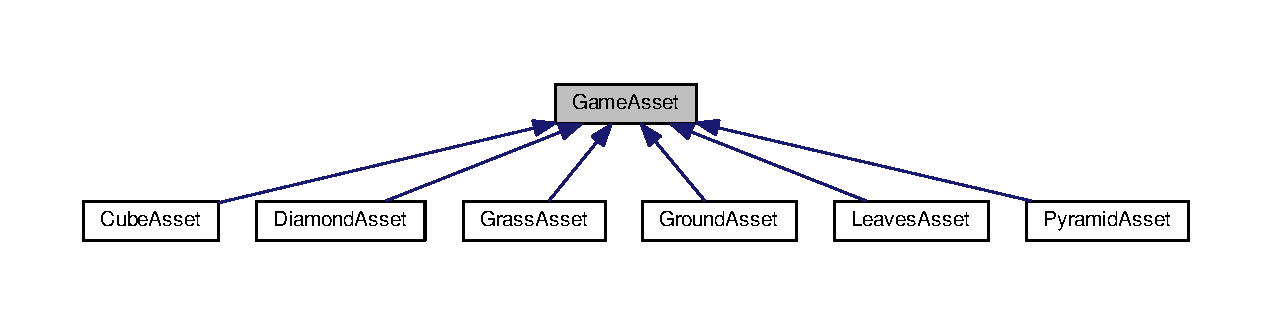
\includegraphics[width=350pt]{class_game_asset__inherit__graph}
\end{center}
\end{figure}
\subsection*{Public Member Functions}
\begin{DoxyCompactItemize}
\item 
\hyperlink{class_game_asset_a9de932075d9b4263e7fb24fbfd163a61}{Game\+Asset} (glm\+::vec3 xyz\+Position, glm\+::vec3 translate\+To, glm\+::vec3 animate\+To, bool translate\+\_\+bool, glm\+::vec3 rotate, bool rotate\+\_\+bool, glm\+::vec3 scale, bool scale\+\_\+bool, string Asset\+Type)
\item 
\hypertarget{class_game_asset_af74bc1c4f6b87a4843217637b75290d4}{}bool {\bfseries Get\+Translate\+Bool} ()\label{class_game_asset_af74bc1c4f6b87a4843217637b75290d4}

\item 
\hypertarget{class_game_asset_ae0a76a50ff3c6c119852c195053c9a38}{}bool {\bfseries Get\+Scale\+Bool} ()\label{class_game_asset_ae0a76a50ff3c6c119852c195053c9a38}

\item 
\hypertarget{class_game_asset_a9fb9187dfca6160898344e79d41de224}{}bool {\bfseries Get\+Rotate\+Bool} ()\label{class_game_asset_a9fb9187dfca6160898344e79d41de224}

\item 
\hypertarget{class_game_asset_a961aa51ca0a9961fc584c0b5d5431300}{}virtual void {\bfseries Draw} (G\+Luint)=0\label{class_game_asset_a961aa51ca0a9961fc584c0b5d5431300}

\item 
\hypertarget{class_game_asset_a992a9c94083ee91bda85a4ec367c4fb3}{}glm\+::vec3 {\bfseries Get\+A\+A\+B\+B} (string check)\label{class_game_asset_a992a9c94083ee91bda85a4ec367c4fb3}

\item 
\hypertarget{class_game_asset_abd0491ffc6a601f8f3c47a2010f14039}{}void {\bfseries Collision\+Detection} (glm\+::vec3 B\+B1\+\_\+\+Max, glm\+::vec3 B\+B1\+\_\+\+Min, glm\+::vec3 B\+B1\+\_\+\+Pos, glm\+::vec3 B\+B2\+\_\+\+Max, glm\+::vec3 B\+B2\+\_\+\+Min, glm\+::vec3 B\+B2\+\_\+\+Pos)\label{class_game_asset_abd0491ffc6a601f8f3c47a2010f14039}

\item 
glm\+::mat4 \hyperlink{class_game_asset_a50a4795382fb55c7513314f82821e444}{Get\+Model} ()
\item 
glm\+::vec3 \hyperlink{class_game_asset_af19b5c6341758ee89c8dfb020eb678f6}{Get\+Translate\+To} ()
\item 
\hypertarget{class_game_asset_a5c0479920e4aa2fea7830a47c1a4e3f3}{}void {\bfseries Translate} (glm\+::vec3 translate\+To)\label{class_game_asset_a5c0479920e4aa2fea7830a47c1a4e3f3}

\end{DoxyCompactItemize}


\subsection{Constructor \& Destructor Documentation}
\hypertarget{class_game_asset_a9de932075d9b4263e7fb24fbfd163a61}{}\index{Game\+Asset@{Game\+Asset}!Game\+Asset@{Game\+Asset}}
\index{Game\+Asset@{Game\+Asset}!Game\+Asset@{Game\+Asset}}
\subsubsection[{Game\+Asset(glm\+::vec3 xyz\+Position, glm\+::vec3 translate\+To, glm\+::vec3 animate\+To, bool translate\+\_\+bool, glm\+::vec3 rotate, bool rotate\+\_\+bool, glm\+::vec3 scale, bool scale\+\_\+bool, string Asset\+Type)}]{\setlength{\rightskip}{0pt plus 5cm}Game\+Asset\+::\+Game\+Asset (
\begin{DoxyParamCaption}
\item[{glm\+::vec3}]{xyz\+Position, }
\item[{glm\+::vec3}]{translate\+To, }
\item[{glm\+::vec3}]{animate\+To, }
\item[{bool}]{translate\+\_\+bool, }
\item[{glm\+::vec3}]{rotate, }
\item[{bool}]{rotate\+\_\+bool, }
\item[{glm\+::vec3}]{scale, }
\item[{bool}]{scale\+\_\+bool, }
\item[{string}]{Asset\+Type}
\end{DoxyParamCaption}
)}\label{class_game_asset_a9de932075d9b4263e7fb24fbfd163a61}
Current Assets Data This gets the current assets data ready to be sent to the Bounding Box Class

Send Data To Bounding Box This Method Sends all the Data from spawning the Asset and sends it to the Bounding Box Class to create the Bounding Box and Manipulate the Asset 

\subsection{Member Function Documentation}
\hypertarget{class_game_asset_a50a4795382fb55c7513314f82821e444}{}\index{Game\+Asset@{Game\+Asset}!Get\+Model@{Get\+Model}}
\index{Get\+Model@{Get\+Model}!Game\+Asset@{Game\+Asset}}
\subsubsection[{Get\+Model()}]{\setlength{\rightskip}{0pt plus 5cm}glm\+::mat4 Game\+Asset\+::\+Get\+Model (
\begin{DoxyParamCaption}
{}
\end{DoxyParamCaption}
)}\label{class_game_asset_a50a4795382fb55c7513314f82821e444}
Get Model This class Gets the Model from the Bounding Box class, This method is normally called by the Draw method in \hyperlink{class_game_asset_manager}{Game\+Asset\+Manager} \hypertarget{class_game_asset_af19b5c6341758ee89c8dfb020eb678f6}{}\index{Game\+Asset@{Game\+Asset}!Get\+Translate\+To@{Get\+Translate\+To}}
\index{Get\+Translate\+To@{Get\+Translate\+To}!Game\+Asset@{Game\+Asset}}
\subsubsection[{Get\+Translate\+To()}]{\setlength{\rightskip}{0pt plus 5cm}glm\+::vec3 Game\+Asset\+::\+Get\+Translate\+To (
\begin{DoxyParamCaption}
{}
\end{DoxyParamCaption}
)}\label{class_game_asset_af19b5c6341758ee89c8dfb020eb678f6}
Get Translate\+To This class Gets the Translate\+To from the Bounding Box class, Which is the current Position of the Asset 

The documentation for this class was generated from the following files\+:\begin{DoxyCompactItemize}
\item 
src/Game\+Asset.\+h\item 
src/Game\+Asset.\+cc\end{DoxyCompactItemize}

\hypertarget{class_game_asset_manager}{}\section{Game\+Asset\+Manager Class Reference}
\label{class_game_asset_manager}\index{Game\+Asset\+Manager@{Game\+Asset\+Manager}}


{\ttfamily \#include $<$Game\+Asset\+Manager.\+h$>$}

\subsection*{Public Member Functions}
\begin{DoxyCompactItemize}
\item 
\hyperlink{class_game_asset_manager_a84d0445928649e0d1e0f8e31ee137b17}{Game\+Asset\+Manager} ()
\item 
virtual \hyperlink{class_game_asset_manager_a1270bd61ecbcca563f079803e40c9b77}{$\sim$\+Game\+Asset\+Manager} ()
\item 
glm\+::vec3 \hyperlink{class_game_asset_manager_a1d9f1f5cc6630a10a0bf358dc2bcddef}{Get\+Camera\+Position} ()
\item 
\hyperlink{class_game_asset_manager_a2c9adcb72faa154c87eadc9bafe5269d}{Game\+Asset\+Manager} (\hyperlink{class_game_asset_manager}{Game\+Asset\+Manager} const \&)
\item 
\hyperlink{class_game_asset_manager_a44f6e2fd6b8ff1dd64e5697f1be7386d}{Game\+Asset\+Manager} (\hyperlink{class_game_asset_manager}{Game\+Asset\+Manager} const \&\&)
\item 
void \hyperlink{class_game_asset_manager_a7c9e4fce50b47b78652e7ff0b4dbb629}{operator=} (\hyperlink{class_game_asset_manager}{Game\+Asset\+Manager})
\item 
void \hyperlink{class_game_asset_manager_ad3de8ff00d55ba04728b1de8213b2349}{Add\+Asset} (std\+::shared\+\_\+ptr$<$ \hyperlink{class_game_asset}{Game\+Asset} $>$)
\begin{DoxyCompactList}\small\item\em Adds a \hyperlink{class_game_asset}{Game\+Asset} to the scene graph. \end{DoxyCompactList}\item 
void \hyperlink{class_game_asset_manager_a32837132bd70a9a9ed537323c2d3d886}{Draw} ()
\begin{DoxyCompactList}\small\item\em Draws each \hyperlink{class_game_asset}{Game\+Asset} in the scene graph. \end{DoxyCompactList}\item 
void \hyperlink{class_game_asset_manager_a459c51716179ef4b931f049be4aa69b4}{Update\+Camera\+Position} (\hyperlink{common_8h_a0da83e35f29c11f7f3c637234f2149f9}{Control} control, int Mouse\+\_\+\+X, int Mouse\+\_\+\+Y)
\end{DoxyCompactItemize}


\subsection{Detailed Description}
\hyperlink{class_game_asset_manager}{Game\+Asset\+Manager} is a container for Game\+Assets. It also provides utility functions to to create a simple Open\+G\+L program that can be used to draw a simple \hyperlink{class_game_asset}{Game\+Asset}. 

\subsection{Constructor \& Destructor Documentation}
\hypertarget{class_game_asset_manager_a84d0445928649e0d1e0f8e31ee137b17}{}\index{Game\+Asset\+Manager@{Game\+Asset\+Manager}!Game\+Asset\+Manager@{Game\+Asset\+Manager}}
\index{Game\+Asset\+Manager@{Game\+Asset\+Manager}!Game\+Asset\+Manager@{Game\+Asset\+Manager}}
\subsubsection[{Game\+Asset\+Manager()}]{\setlength{\rightskip}{0pt plus 5cm}Game\+Asset\+Manager\+::\+Game\+Asset\+Manager (
\begin{DoxyParamCaption}
{}
\end{DoxyParamCaption}
)\hspace{0.3cm}{\ttfamily [explicit]}}\label{class_game_asset_manager_a84d0445928649e0d1e0f8e31ee137b17}
Creates a \hyperlink{class_game_asset_manager}{Game\+Asset\+Manager} to load the correct shaders based on the Application\+Mode. 
\begin{DoxyCode}
7                                    \{
8         std::string vertex\_shader(\textcolor{stringliteral}{"shaders/translate.vs"});
9         std::string fragment\_shader(\textcolor{stringliteral}{"shaders/fragment.fs"});
10 
11         program\_token = CreateGLProgram(vertex\_shader, fragment\_shader);
12 \}
\end{DoxyCode}
\hypertarget{class_game_asset_manager_a1270bd61ecbcca563f079803e40c9b77}{}\index{Game\+Asset\+Manager@{Game\+Asset\+Manager}!````~Game\+Asset\+Manager@{$\sim$\+Game\+Asset\+Manager}}
\index{````~Game\+Asset\+Manager@{$\sim$\+Game\+Asset\+Manager}!Game\+Asset\+Manager@{Game\+Asset\+Manager}}
\subsubsection[{$\sim$\+Game\+Asset\+Manager()}]{\setlength{\rightskip}{0pt plus 5cm}Game\+Asset\+Manager\+::$\sim$\+Game\+Asset\+Manager (
\begin{DoxyParamCaption}
{}
\end{DoxyParamCaption}
)\hspace{0.3cm}{\ttfamily [virtual]}}\label{class_game_asset_manager_a1270bd61ecbcca563f079803e40c9b77}
Deletes a \hyperlink{class_game_asset_manager}{Game\+Asset\+Manager}, in particular it will clean up any modifications to the Open\+G\+L state. 
\begin{DoxyCode}
22                                     \{
23         glDeleteProgram(program\_token);
24 \}
\end{DoxyCode}
\hypertarget{class_game_asset_manager_a2c9adcb72faa154c87eadc9bafe5269d}{}\index{Game\+Asset\+Manager@{Game\+Asset\+Manager}!Game\+Asset\+Manager@{Game\+Asset\+Manager}}
\index{Game\+Asset\+Manager@{Game\+Asset\+Manager}!Game\+Asset\+Manager@{Game\+Asset\+Manager}}
\subsubsection[{Game\+Asset\+Manager(\+Game\+Asset\+Manager const \&)}]{\setlength{\rightskip}{0pt plus 5cm}Game\+Asset\+Manager\+::\+Game\+Asset\+Manager (
\begin{DoxyParamCaption}
\item[{{\bf Game\+Asset\+Manager} const \&}]{the\+\_\+manager}
\end{DoxyParamCaption}
)}\label{class_game_asset_manager_a2c9adcb72faa154c87eadc9bafe5269d}
Unimplemented copy constructor -- this means that the \hyperlink{class_game_asset_manager}{Game\+Asset\+Manager} may not work as you\textquotesingle{}d expect when being copied. 
\begin{DoxyCode}
30                                                                       \{
31   \textcolor{comment}{// TODO: implement this}
32 \}
\end{DoxyCode}
\hypertarget{class_game_asset_manager_a44f6e2fd6b8ff1dd64e5697f1be7386d}{}\index{Game\+Asset\+Manager@{Game\+Asset\+Manager}!Game\+Asset\+Manager@{Game\+Asset\+Manager}}
\index{Game\+Asset\+Manager@{Game\+Asset\+Manager}!Game\+Asset\+Manager@{Game\+Asset\+Manager}}
\subsubsection[{Game\+Asset\+Manager(\+Game\+Asset\+Manager const \&\&)}]{\setlength{\rightskip}{0pt plus 5cm}Game\+Asset\+Manager\+::\+Game\+Asset\+Manager (
\begin{DoxyParamCaption}
\item[{{\bf Game\+Asset\+Manager} const \&\&}]{the\+\_\+manager}
\end{DoxyParamCaption}
)}\label{class_game_asset_manager_a44f6e2fd6b8ff1dd64e5697f1be7386d}
Unimplemented move constructor -- this unimplemented method violates the C++11 move semantics for \hyperlink{class_game_asset_manager}{Game\+Asset\+Manager}. 
\begin{DoxyCode}
38                                                                        \{
39   \textcolor{comment}{// TODO: implement this}
40 \}
\end{DoxyCode}


\subsection{Member Function Documentation}
\hypertarget{class_game_asset_manager_ad3de8ff00d55ba04728b1de8213b2349}{}\index{Game\+Asset\+Manager@{Game\+Asset\+Manager}!Add\+Asset@{Add\+Asset}}
\index{Add\+Asset@{Add\+Asset}!Game\+Asset\+Manager@{Game\+Asset\+Manager}}
\subsubsection[{Add\+Asset(std\+::shared\+\_\+ptr$<$ Game\+Asset $>$)}]{\setlength{\rightskip}{0pt plus 5cm}void Game\+Asset\+Manager\+::\+Add\+Asset (
\begin{DoxyParamCaption}
\item[{std\+::shared\+\_\+ptr$<$ {\bf Game\+Asset} $>$}]{game\+\_\+asset}
\end{DoxyParamCaption}
)}\label{class_game_asset_manager_ad3de8ff00d55ba04728b1de8213b2349}


Adds a \hyperlink{class_game_asset}{Game\+Asset} to the scene graph. 


\begin{DoxyCode}
53                                                                    \{
54         draw\_list.push\_back(game\_asset);
55 \}
\end{DoxyCode}
\hypertarget{class_game_asset_manager_a32837132bd70a9a9ed537323c2d3d886}{}\index{Game\+Asset\+Manager@{Game\+Asset\+Manager}!Draw@{Draw}}
\index{Draw@{Draw}!Game\+Asset\+Manager@{Game\+Asset\+Manager}}
\subsubsection[{Draw()}]{\setlength{\rightskip}{0pt plus 5cm}void Game\+Asset\+Manager\+::\+Draw (
\begin{DoxyParamCaption}
{}
\end{DoxyParamCaption}
)}\label{class_game_asset_manager_a32837132bd70a9a9ed537323c2d3d886}


Draws each \hyperlink{class_game_asset}{Game\+Asset} in the scene graph. 

Camera/\+Asset Matrix

This class links the camera matrix to the Draw method as well as the new position the Game Assets are set.

Collision Check

Checks whether one block collides with the other Block 
\begin{DoxyCode}
60                             \{
61     \textcolor{keywordflow}{for}(\textcolor{keyword}{auto} ga: draw\_list)
62     \{
69         glm::mat4 Camera\_Model(1.0f);
70 
71         GLuint Camera\_Projection\_Link = glGetUniformLocation(program\_token, \textcolor{stringliteral}{"Camera\_Projection"});
72         GLuint Camera\_View\_Link = glGetUniformLocation(program\_token, \textcolor{stringliteral}{"Camera\_View"});
73         GLuint Camera\_Model\_Link = glGetUniformLocation(program\_token, \textcolor{stringliteral}{"Camera\_Model"});
74 
75                 Camera\_Projection = glm::perspective(45.0f, 16.0f/10.0f, 0.1f, 1000.0f);
76                 
77         glUniformMatrix4fv(Camera\_Projection\_Link, 1, GL\_FALSE, &Camera\_Projection[0][0]);
78         glUniformMatrix4fv(Camera\_View\_Link, 1, GL\_FALSE, &Camera\_View[0][0]);
79 
80                 Camera\_Model = ga->GetModel();
81         glUniformMatrix4fv(Camera\_Model\_Link, 1, GL\_FALSE, &Camera\_Model[0][0]);
82         
88                 \textcolor{comment}{//std::shared\_ptr<GameAsset> game\_asset = std::make\_shared<GameAsset>();}
89                 
90                 \textcolor{keywordflow}{if}( ga->GetTranslateBool() == \textcolor{keyword}{true} || ga->GetScaleBool() == \textcolor{keyword}{true} || ga->GetRotateBool() == 
      true )\{
91                         BB1\_Max = ga->GetAABB(\textcolor{stringliteral}{"Max"});
92                         BB1\_Min = ga->GetAABB(\textcolor{stringliteral}{"Min"});
93                         BB1\_Pos = ga->GetTranslateTo();
94                         
95                         \textcolor{keywordflow}{for}(\textcolor{keyword}{auto} ga2: draw\_list) \{
96                                 BB2\_Max = ga2->GetAABB(\textcolor{stringliteral}{"Max"});
97                                 BB2\_Min = ga2->GetAABB(\textcolor{stringliteral}{"Min"});
98                                 BB2\_Pos = ga2->GetTranslateTo();
99                                 camera->CollisionDetection(BB2\_Max, BB2\_Min);
100                                 \textcolor{keywordflow}{if}(BB1\_Pos != BB2\_Pos) \{
101                                          ga->CollisionDetection(BB1\_Max, BB1\_Min, BB1\_Pos, BB2\_Max, BB2\_Min
      , BB2\_Pos);
102                                 \}
103                         \}
104                 \}
105                 ga->Draw(program\_token);
106     \}
107 \}
\end{DoxyCode}
\hypertarget{class_game_asset_manager_a1d9f1f5cc6630a10a0bf358dc2bcddef}{}\index{Game\+Asset\+Manager@{Game\+Asset\+Manager}!Get\+Camera\+Position@{Get\+Camera\+Position}}
\index{Get\+Camera\+Position@{Get\+Camera\+Position}!Game\+Asset\+Manager@{Game\+Asset\+Manager}}
\subsubsection[{Get\+Camera\+Position()}]{\setlength{\rightskip}{0pt plus 5cm}glm\+::vec3 Game\+Asset\+Manager\+::\+Get\+Camera\+Position (
\begin{DoxyParamCaption}
{}
\end{DoxyParamCaption}
)}\label{class_game_asset_manager_a1d9f1f5cc6630a10a0bf358dc2bcddef}
\hypertarget{class_game_asset_manager_a7c9e4fce50b47b78652e7ff0b4dbb629}{}\index{Game\+Asset\+Manager@{Game\+Asset\+Manager}!operator=@{operator=}}
\index{operator=@{operator=}!Game\+Asset\+Manager@{Game\+Asset\+Manager}}
\subsubsection[{operator=(\+Game\+Asset\+Manager)}]{\setlength{\rightskip}{0pt plus 5cm}void Game\+Asset\+Manager\+::operator= (
\begin{DoxyParamCaption}
\item[{{\bf Game\+Asset\+Manager}}]{}
\end{DoxyParamCaption}
)}\label{class_game_asset_manager_a7c9e4fce50b47b78652e7ff0b4dbb629}
Unimplemented assisgnment operator -- violates the expected semantics for assignment in C++11. 
\begin{DoxyCode}
46                                                  \{
47   \textcolor{comment}{// TODO: implement this}
48 \}
\end{DoxyCode}
\hypertarget{class_game_asset_manager_a459c51716179ef4b931f049be4aa69b4}{}\index{Game\+Asset\+Manager@{Game\+Asset\+Manager}!Update\+Camera\+Position@{Update\+Camera\+Position}}
\index{Update\+Camera\+Position@{Update\+Camera\+Position}!Game\+Asset\+Manager@{Game\+Asset\+Manager}}
\subsubsection[{Update\+Camera\+Position(\+Control control, int Mouse\+\_\+\+X, int Mouse\+\_\+\+Y)}]{\setlength{\rightskip}{0pt plus 5cm}void Game\+Asset\+Manager\+::\+Update\+Camera\+Position (
\begin{DoxyParamCaption}
\item[{{\bf Control}}]{control, }
\item[{int}]{Mouse\+\_\+\+X, }
\item[{int}]{Mouse\+\_\+\+Y}
\end{DoxyParamCaption}
)}\label{class_game_asset_manager_a459c51716179ef4b931f049be4aa69b4}

\begin{DoxyCode}
14                                                                                      \{
15         Camera\_View = camera->UpdateCameraPosition(control, Mouse\_X, Mouse\_Y);
16   \}
\end{DoxyCode}


The documentation for this class was generated from the following files\+:\begin{DoxyCompactItemize}
\item 
src/\hyperlink{_game_asset_manager_8h}{Game\+Asset\+Manager.\+h}\item 
src/\hyperlink{_game_asset_manager_8cc}{Game\+Asset\+Manager.\+cc}\end{DoxyCompactItemize}

\hypertarget{class_game_loop}{}\section{Game\+Loop Class Reference}
\label{class_game_loop}\index{Game\+Loop@{Game\+Loop}}
\subsection*{Public Member Functions}
\begin{DoxyCompactItemize}
\item 
\hypertarget{class_game_loop_afcbeaf01f4a6d443753ccabbadbec8d7}{}std\+::shared\+\_\+ptr$<$ S\+D\+L\+\_\+\+Window $>$ {\bfseries Init\+World} ()\label{class_game_loop_afcbeaf01f4a6d443753ccabbadbec8d7}

\item 
\hypertarget{class_game_loop_a5034124015cce5b8ecedae9f906b897b}{}void {\bfseries Draw} (const std\+::shared\+\_\+ptr$<$ S\+D\+L\+\_\+\+Window $>$ \&window, const std\+::shared\+\_\+ptr$<$ \hyperlink{class_game_world}{Game\+World} $>$ \&game\+\_\+world)\label{class_game_loop_a5034124015cce5b8ecedae9f906b897b}

\item 
void \hyperlink{class_game_loop_a6d84f749fa38ca86039353245d77461c}{Run} ()
\end{DoxyCompactItemize}


\subsection{Member Function Documentation}
\hypertarget{class_game_loop_a6d84f749fa38ca86039353245d77461c}{}\index{Game\+Loop@{Game\+Loop}!Run@{Run}}
\index{Run@{Run}!Game\+Loop@{Game\+Loop}}
\subsubsection[{Run()}]{\setlength{\rightskip}{0pt plus 5cm}void Game\+Loop\+::\+Run (
\begin{DoxyParamCaption}
{}
\end{DoxyParamCaption}
)}\label{class_game_loop_a6d84f749fa38ca86039353245d77461c}
Add the main event loop. Detects Keyboard and Mouse Sends Data to \hyperlink{class_game_world}{Game\+World} \hyperlink{class_camera}{Camera} Controls

The documentation for this class was generated from the following files\+:\begin{DoxyCompactItemize}
\item 
src/Game\+Loop.\+h\item 
src/Game\+Loop.\+cc\end{DoxyCompactItemize}

\hypertarget{class_game_world}{}\section{Game\+World Class Reference}
\label{class_game_world}\index{Game\+World@{Game\+World}}


{\ttfamily \#include $<$Game\+World.\+h$>$}

\subsection*{Public Member Functions}
\begin{DoxyCompactItemize}
\item 
\hyperlink{class_game_world_a681994123c12833d43c957d6cfb33765}{Game\+World} ()
\item 
void \hyperlink{class_game_world_a275418607d8286979b276f165ad5876b}{Draw} ()
\begin{DoxyCompactList}\small\item\em Calling \hyperlink{class_game_world_a275418607d8286979b276f165ad5876b}{Draw()}. will draw the entire world. \end{DoxyCompactList}\item 
void \hyperlink{class_game_world_a9fa019e8e1d4bbc8e8c101352a73b17a}{Update\+Camera\+Position} (\hyperlink{common_8h_a0da83e35f29c11f7f3c637234f2149f9}{Control} control, int Mouse\+\_\+\+X, int Mouse\+\_\+\+Y)
\end{DoxyCompactItemize}
\subsection*{Public Attributes}
\begin{DoxyCompactItemize}
\item 
double \hyperlink{class_game_world_a54ccf4cf03172ab8779e9c326c8846ed}{Minimum\+Number} = 0.\+50
\item 
double \hyperlink{class_game_world_a1cddcf233625a98581eaeb9fd7c8c574}{Maximum\+Number} = 1.\+00
\item 
double \hyperlink{class_game_world_a56652cc9880b3ba1be61395066c863c3}{Random} = (double)rand() / R\+A\+N\+D\+\_\+\+M\+A\+X
\item 
G\+Lfloat \hyperlink{class_game_world_a9bf4eb977e6ab9299aaef1345c4fa4dd}{Mouse\+\_\+\+Sensitivity} = 0.\+05f
\begin{DoxyCompactList}\small\item\em Call Camera\+\_\+\+Control. will move in specfic direction. \end{DoxyCompactList}\item 
G\+Lfloat \hyperlink{class_game_world_ae8ab2ac372729cec44ea316f6bdf45ca}{Player\+\_\+\+Speed} = 1.\+0
\item 
G\+Lfloat \hyperlink{class_game_world_a7f4911dda9b3b4e4eb03ece87e16cd96}{Camera\+\_\+\+Horizontal} = 0.\+0
\item 
G\+Lfloat \hyperlink{class_game_world_a26658e739c4d267b1be35ed820089931}{Camera\+\_\+\+Vertical} = 0.\+0
\item 
G\+Lfloat \hyperlink{class_game_world_ad07b1f650edb08ddb05e74a22588bda0}{Camera\+\_\+\+X\+\_\+\+Position} = 0
\item 
G\+Lfloat \hyperlink{class_game_world_ae3e7cab30494ff5a8e91dfa7406deb16}{Camera\+\_\+\+Y\+\_\+\+Position} = 2
\item 
G\+Lfloat \hyperlink{class_game_world_ad993ea24fbacfc98410894078e916927}{Camera\+\_\+\+Z\+\_\+\+Position} = 0
\item 
G\+Lfloat \hyperlink{class_game_world_a734c19bd480aef2a7af005e170d3d523}{Old\+\_\+\+Camera\+\_\+\+X\+\_\+\+Position}
\item 
G\+Lfloat \hyperlink{class_game_world_ac1c9de2db7cb175f7a039a9f825190fc}{Old\+\_\+\+Camera\+\_\+\+Y\+\_\+\+Position}
\item 
G\+Lfloat \hyperlink{class_game_world_acf69fc81410f4bb31d03b7551eb0bced}{Old\+\_\+\+Camera\+\_\+\+Z\+\_\+\+Position}
\item 
glm\+::vec3 \hyperlink{class_game_world_ad80e597474ea4c52a583e81788187571}{Camera\+\_\+\+Position} = glm\+::vec3(\hyperlink{class_game_world_ad07b1f650edb08ddb05e74a22588bda0}{Camera\+\_\+\+X\+\_\+\+Position}, \hyperlink{class_game_world_ae3e7cab30494ff5a8e91dfa7406deb16}{Camera\+\_\+\+Y\+\_\+\+Position}, \hyperlink{class_game_world_ad993ea24fbacfc98410894078e916927}{Camera\+\_\+\+Z\+\_\+\+Position})
\item 
glm\+::vec3 \hyperlink{class_game_world_ade0aa1baaba6ac54674638cef313c0bb}{Old\+\_\+\+Camera\+\_\+\+Position} = \hyperlink{class_game_world_ad80e597474ea4c52a583e81788187571}{Camera\+\_\+\+Position}
\item 
glm\+::vec3 \hyperlink{class_game_world_a8dd30ba92e7fa9b9b05075e31d1e7dd8}{Movement\+\_\+\+Z}
\item 
glm\+::vec3 \hyperlink{class_game_world_a968eb29424b68f7cd79a5896c62e944d}{Movement\+\_\+\+X}
\end{DoxyCompactItemize}


\subsection{Detailed Description}
\hyperlink{class_game_world}{Game\+World} allows us to separate the management of the game world from the nuts and bolts of game loop initialisation. The \hyperlink{class_game_world}{Game\+World} currently has a very simplified scene graph consisiting of a single \hyperlink{class_game_asset_manager}{Game\+Asset\+Manager}. 

\subsection{Constructor \& Destructor Documentation}
\hypertarget{class_game_world_a681994123c12833d43c957d6cfb33765}{}\index{Game\+World@{Game\+World}!Game\+World@{Game\+World}}
\index{Game\+World@{Game\+World}!Game\+World@{Game\+World}}
\subsubsection[{Game\+World()}]{\setlength{\rightskip}{0pt plus 5cm}Game\+World\+::\+Game\+World (
\begin{DoxyParamCaption}
{}
\end{DoxyParamCaption}
)\hspace{0.3cm}{\ttfamily [explicit]}}\label{class_game_world_a681994123c12833d43c957d6cfb33765}
We thread the Application\+Mode through the \hyperlink{class_game_world}{Game\+World} ss we want to read it in from the user. Threading the state through the various function calls is preferable (in this case) to having some kind of global state. 2\+D array for world space. 2\+D array which acts like the world space for the game, so depending on what number is stored within the array would change which blocks spawn within this small 20 by 20 world, I would like to improve the size of the array in the future but as of now I don\textquotesingle{}t think it\textquotesingle{}s to important.

1-\/$>$ 2 high Ground Blocks.

2-\/$>$ A 1 high Cube with a Diamond on top.

3-\/$>$ A 2 high Cube with a Diamond on top.

4-\/$>$ A Tree.

5-\/$>$ A Cube with a Pyramid on top.

6-\/$>$ A Pyramid.

7-\/$>$ Somewhat Random Grass.

Spawning different Voxels. Spawns all the Voxel assets I made just outside the array space, Just so you can view each voxel on it\textquotesingle{}s own. Each of them has random animations or changes to them to show off the animation.

Spawns Ground. Spawns the Voxel \hyperlink{class_ground_asset}{Ground\+Asset} so it creates a two tall ground world for the world

Spawning Small Diamond Tower. Spawns the Voxel \hyperlink{class_ground_asset}{Ground\+Asset} so it creates a two tall ground world for the world Spawns the Cube \& Diamond asset on top to create a small tower with a diamond on top

Spawning Taller Diamond Tower. Spawns the Voxel \hyperlink{class_ground_asset}{Ground\+Asset} so it creates a two tall ground world for the world Spawns the Cube \& Diamond asset on top to create a taller tower with a diamond on top

Tree Spawn. Spawns the Voxel \hyperlink{class_ground_asset}{Ground\+Asset} so it creates a two tall ground world for the world Spawns the multiple voxels to create a shape of a simple tree, It uses multiple layers to get each seperate part to spawn.

Spawns Pyramid Tower. Spawns the Voxel \hyperlink{class_ground_asset}{Ground\+Asset} so it creates a two tall ground world for the world Spawns the Cube \& Pyramid asset on top to create a small tower with a diamond on top

Spawns Pyramid. Spawns the Voxel \hyperlink{class_ground_asset}{Ground\+Asset} so it creates a two tall ground world for the world Spawns Pyramid asset on top of the ground asset

Grass Spawn. Spawns the Voxel \hyperlink{class_ground_asset}{Ground\+Asset} so it creates a two tall ground world for the world Spawns somewhat randomly multiple grass assets on top/ slighlty inside the ground asset To create the view of grass.
\begin{DoxyCode}
3                      : asset\_manager (make\_shared<GameAssetManager>())  \{ 
4   \textcolor{keywordtype}{int} pointX,pointY;
5   \textcolor{keywordtype}{int} pointZ = 1;
6   \textcolor{keywordtype}{int} worldX = 25;
7   \textcolor{keywordtype}{int} worldY = 25;
8 
30   \textcolor{keywordtype}{int} world[25][25] = \{
31   \{1,1,1,1,1,1,1,1,1,1,1,1,1,1,1,1,1,1,1,1,1,1,1,1,1\},
32   \{1,2,1,1,1,1,1,1,1,1,1,1,5,1,1,1,7,1,1,1,7,1,1,2,1\},
33   \{1,1,1,1,1,1,1,7,1,1,1,1,1,1,1,1,1,1,1,1,1,1,1,1,1\},
34   \{1,1,1,1,7,1,1,1,1,7,1,1,1,1,1,1,1,1,7,1,1,1,1,1,1\},
35   \{1,1,1,1,1,1,1,1,1,1,1,1,1,1,1,1,1,1,1,1,1,1,1,1,1\},
36   \{1,1,1,1,1,3,1,1,1,1,1,7,1,1,1,7,1,1,1,3,1,1,1,1,1\},
37   \{1,1,7,1,7,1,1,1,1,1,1,1,1,1,1,1,1,1,1,1,1,1,1,1,1\},
38   \{1,1,1,1,1,1,1,7,1,1,1,1,6,1,1,1,1,7,1,1,1,7,1,1,1\},
39   \{1,1,1,1,1,1,1,1,1,1,1,1,1,1,1,1,1,1,1,1,1,1,1,1,1\},
40   \{1,1,1,1,7,1,7,1,1,1,7,1,1,1,1,1,1,1,7,1,7,1,1,1,1\},
41   \{1,1,1,1,1,1,1,1,1,1,1,1,1,1,7,1,1,1,1,1,1,1,1,1,1\},
42   \{1,1,1,1,1,1,1,7,1,1,7,1,1,1,1,1,1,1,1,1,1,1,1,1,1\},
43   \{1,5,1,7,1,1,1,6,1,1,1,1,4,1,1,1,1,6,1,1,1,1,1,5,1\},
44   \{1,1,1,1,1,1,1,1,1,1,1,1,1,1,7,1,1,7,1,1,1,1,1,1,1\},
45   \{1,1,1,1,1,7,1,1,1,1,7,1,1,1,1,1,1,1,1,1,1,7,1,1,1\},
46   \{1,1,1,1,1,1,1,1,1,1,1,1,1,1,1,1,1,7,1,1,1,1,1,1,1\},
47   \{1,1,1,1,1,1,1,1,1,1,1,1,1,1,1,1,1,1,1,1,1,7,1,1,1\},
48   \{1,1,1,1,1,1,7,1,1,1,1,1,6,7,7,1,1,1,1,1,1,1,1,1,1\},
49   \{1,1,1,7,1,1,1,1,1,1,1,1,1,1,1,1,1,1,1,1,1,7,1,1,1\},
50   \{1,1,1,1,1,3,1,1,7,1,1,1,1,1,1,1,1,1,1,3,1,1,7,1,1\},
51   \{1,1,1,1,1,1,1,1,1,1,1,1,1,1,1,1,1,7,1,1,1,1,1,1,1\},
52   \{1,1,1,1,1,1,7,1,1,1,7,1,1,7,1,1,7,1,1,1,1,1,1,1,1\},
53   \{1,1,1,1,1,1,1,1,7,1,1,1,1,1,1,1,1,1,1,7,1,1,7,1,1\},
54   \{1,2,1,1,1,1,1,1,1,1,1,1,5,1,1,7,1,1,1,1,1,1,1,2,1\},
55   \{1,1,1,1,1,1,1,1,1,1,1,1,1,1,1,1,1,1,1,1,1,1,1,1,1\}        
56   \};
57                    
58                                    
59       
60         
67 
68         asset\_manager->AddAsset(make\_shared<GroundAsset>(Spawn, glm::vec3(1.0f ,2.00f, -4.0f),
69                                                          glm::vec3(1.0f ,2.00f, -4.0f), \textcolor{keyword}{false},
70                                                          No\_Rotation, \textcolor{keyword}{false},
71                                                          Giant\_Size, \textcolor{keyword}{true}, \textcolor{stringliteral}{"Ground"}));
72         asset\_manager->AddAsset(make\_shared<CubeAsset>(Spawn, glm::vec3(3.0f ,2.00f, -4.0f),
73                                                        glm::vec3(3.0f,2.0f,-4.0f), \textcolor{keyword}{false},
74                                                        Fast\_Rotation, \textcolor{keyword}{true},
75                                                        Normal\_Size, \textcolor{keyword}{false}, \textcolor{stringliteral}{"Cube"}));
76         asset\_manager->AddAsset(make\_shared<LeavesAsset>(Spawn, glm::vec3(5.0f ,2.00f, -4.0f),
77                                                          glm::vec3(5.0f,2.0f,-4.0f), \textcolor{keyword}{false},
78                                                          glm::vec3(0.1f,0.1f,0.1f), \textcolor{keyword}{true},
79                                                          glm::vec3(1.1f,1.1f,1.1f), \textcolor{keyword}{true}, \textcolor{stringliteral}{"Leaves"}));
80                                                          
81         asset\_manager->AddAsset(make\_shared<DiamondAsset>(Spawn, glm::vec3(7.0f ,2.0f, -4.0f),
82                                                           glm::vec3(7.0f, 2.0f, -15.0f), \textcolor{keyword}{true},
83                                                           No\_Rotation, \textcolor{keyword}{false},
84                                                           Normal\_Size, \textcolor{keyword}{false}, \textcolor{stringliteral}{"Diamond"}));
85         asset\_manager->AddAsset(make\_shared<CubeAsset>(Spawn, glm::vec3(7.0f ,2.0f, -13.0f),
86                                                           glm::vec3(7.0f, 2.0f, -13.0f), \textcolor{keyword}{false},
87                                                           Normal\_Rotation, \textcolor{keyword}{true},
88                                                           Double\_Size, \textcolor{keyword}{true}, \textcolor{stringliteral}{"Cube"}));
89                                                           
90         asset\_manager->AddAsset(make\_shared<PyramidAsset>(Spawn, glm::vec3(9.0f ,1.50f, -4.0f),
91                                                           glm::vec3(9.0f,1.50f,-4.0f), \textcolor{keyword}{false},
92                                                           No\_Rotation, \textcolor{keyword}{false},
93                                                           Double\_Size, \textcolor{keyword}{false}, \textcolor{stringliteral}{"Pyramid"})); 
94         asset\_manager->AddAsset(make\_shared<GrassAsset>(Spawn, glm::vec3(11.0f,1.50f, -4.0f), 
95                                                         glm::vec3(11.0f,1.50f,-4.0f), \textcolor{keyword}{false},
96                                                         No\_Rotation, \textcolor{keyword}{false},
97                                                         Giant\_Size, \textcolor{keyword}{true}, \textcolor{stringliteral}{"Grass"}));
98         asset\_manager->AddAsset(make\_shared<CubeAsset>(Spawn, glm::vec3(0.0f ,10.0f, 0.0f),
99                                                          glm::vec3(0.0f,0.0f,0.0f), \textcolor{keyword}{true},
100                                                          No\_Rotation, \textcolor{keyword}{false},
101                                                          Normal\_Size, \textcolor{keyword}{false}, \textcolor{stringliteral}{"Cube"}));
102         asset\_manager->AddAsset(make\_shared<CubeAsset>(Spawn, glm::vec3(0.0f ,0.0f, 0.0f),
103                                                        glm::vec3(0.0f,10.0f,0.0f), \textcolor{keyword}{true},
104                                                          No\_Rotation, \textcolor{keyword}{false}, 
105                                                          Normal\_Size, \textcolor{keyword}{false}, \textcolor{stringliteral}{"Cube"}));
106         asset\_manager->AddAsset(make\_shared<DiamondAsset>(Spawn, glm::vec3(12.0f,12.0f,12.0f), 
107                                                           glm::vec3(12.0f,12.0f,12.0f), \textcolor{keyword}{false},
108                                                           Normal\_Rotation, \textcolor{keyword}{true},
109                                                           Normal\_Size, \textcolor{keyword}{false}, \textcolor{stringliteral}{"Diamond"})); 
110                                                           
111         asset\_manager->AddAsset(make\_shared<CubeAsset>(Spawn, glm::vec3(-10.0f ,5.0f, -5.0f),
112                                                          glm::vec3(0.0f,5.0f,-5.0f), \textcolor{keyword}{true},
113                                                          No\_Rotation, \textcolor{keyword}{false},
114                                                          Normal\_Size, \textcolor{keyword}{false}, \textcolor{stringliteral}{"Cube"}));
115         asset\_manager->AddAsset(make\_shared<CubeAsset>(Spawn, glm::vec3(0.0f ,5.0f, -5.0f),
116                                                        glm::vec3(-10.0f,5.0f,-5.0f), \textcolor{keyword}{true},
117                                                          No\_Rotation, \textcolor{keyword}{false}, 
118                                                          Normal\_Size, \textcolor{keyword}{false}, \textcolor{stringliteral}{"Cube"})); 
119         asset\_manager->AddAsset(make\_shared<GroundAsset>(Spawn, glm::vec3(15.0f ,2.00f, 30.0f),
120                                                          glm::vec3(25.0f ,2.00f, 25.0f), \textcolor{keyword}{false},
121                                                          No\_Rotation, \textcolor{keyword}{false},
122                                                          Giant\_Size, \textcolor{keyword}{true}, \textcolor{stringliteral}{"Ground"}));
123         asset\_manager->AddAsset(make\_shared<GroundAsset>(Spawn, glm::vec3(9.0f ,2.00f, 30.0f),
124                                                          glm::vec3(25.0f ,2.00f, 25.0f), \textcolor{keyword}{false},
125                                                          No\_Rotation, \textcolor{keyword}{false},
126                                                          Giant\_Size, \textcolor{keyword}{true}, \textcolor{stringliteral}{"Ground"}));
127    \textcolor{comment}{//AddAsset Layout }
128    \textcolor{comment}{//This adds the asset to the game asset manager which draws it to the screen}
129    \textcolor{comment}{//}
130    \textcolor{comment}{//  asset\_manager->AddAsset(make\_shared<CubeAsset>(Spawn, Translate}
131    \textcolor{comment}{//                                                 AnimateTo , Bool,}
132    \textcolor{comment}{//                                                 Rotation, Bool,}
133    \textcolor{comment}{//                                                 Scale, Bool));  }
135 \textcolor{comment}{}
136   \textcolor{keywordflow}{for}( pointX=0; pointX<worldX; pointX++)\{
137    \textcolor{keywordflow}{for} (pointY=0; pointY<worldY; pointY++)\{
138     \textcolor{keywordflow}{if}( world[pointY][pointX] == 1 || world[pointY][pointX] == 2 || world[pointY][pointX] == 3 || world[
      pointY][pointX] == 4 || world[pointY][pointX] == 5 || world[pointY][pointX] == 6 || world[pointY][pointX] == 7)
      \{          
143             asset\_manager->AddAsset(make\_shared<GroundAsset>(Spawn, glm::vec3((pointX),-1.00f,(pointZ*
      pointY)),
144                                                              glm::vec3(0.0f,0.0f,0.0f), \textcolor{keyword}{false},
145                                                              No\_Rotation, \textcolor{keyword}{false},
146                                                              Normal\_Size, \textcolor{keyword}{false}, \textcolor{stringliteral}{"Ground"}));
147             asset\_manager->AddAsset(make\_shared<GroundAsset>(Spawn, glm::vec3((pointX),-2.00f,(pointZ*
      pointY)),
148                                                              glm::vec3(0.0f,0.0f,0.0f), \textcolor{keyword}{false},
149                                                              No\_Rotation, \textcolor{keyword}{false},
150                                                              Normal\_Size, \textcolor{keyword}{false}, \textcolor{stringliteral}{"Ground"}));
151    \}
152    \textcolor{keywordflow}{if}( world[pointY][pointX] == 2)\{
158             asset\_manager->AddAsset(make\_shared<GroundAsset>(Spawn, glm::vec3((pointX),-1.00f,(pointZ*
      pointY)),
159                                                              glm::vec3(0.0f,0.0f,0.0f), \textcolor{keyword}{false},
160                                                              No\_Rotation, \textcolor{keyword}{false},
161                                                              Normal\_Size, \textcolor{keyword}{false}, \textcolor{stringliteral}{"Ground"}));
162             asset\_manager->AddAsset(make\_shared<GroundAsset>(Spawn, glm::vec3((pointX),-1.00f,(pointZ*
      pointY)),
163                                                              glm::vec3(0.0f,0.0f,0.0f), \textcolor{keyword}{false},
164                                                              No\_Rotation, \textcolor{keyword}{false},
165                                                              Normal\_Size, \textcolor{keyword}{false}, \textcolor{stringliteral}{"Ground"}));
166             asset\_manager->AddAsset(make\_shared<CubeAsset>(Spawn, glm::vec3((pointX),0.00f,(pointZ*pointY))
      , 
167                                                            glm::vec3(0.0f,0.0f,0.0f), \textcolor{keyword}{false},
168                                                            No\_Rotation, \textcolor{keyword}{false},
169                                                            Double\_Size, \textcolor{keyword}{true}, \textcolor{stringliteral}{"Cube"}));
170             asset\_manager->AddAsset(make\_shared<DiamondAsset>(Spawn, glm::vec3((pointX),1.0f,(pointZ*pointY
      )), 
171                                                               glm::vec3(12.0f,15.0f,12.0f), \textcolor{keyword}{true},
172                                                               Normal\_Rotation, \textcolor{keyword}{true},
173                                                               Normal\_Size, \textcolor{keyword}{false}, \textcolor{stringliteral}{"Diamond"}));
174    \}
175    \textcolor{keywordflow}{else} \textcolor{keywordflow}{if}( world[pointY][pointX] == 3)\{
181             asset\_manager->AddAsset(make\_shared<GroundAsset>(Spawn, glm::vec3((pointX),-1.00f,(pointZ*
      pointY)),
182                                                              glm::vec3(0.0f,0.0f,0.0f), \textcolor{keyword}{false},
183                                                              No\_Rotation, \textcolor{keyword}{false},
184                                                              Normal\_Size, \textcolor{keyword}{false}, \textcolor{stringliteral}{"Ground"}));
185             asset\_manager->AddAsset(make\_shared<GroundAsset>(Spawn, glm::vec3((pointX),-1.00f,(pointZ*
      pointY)),
186                                                              glm::vec3(0.0f,0.0f,0.0f), \textcolor{keyword}{false},
187                                                              No\_Rotation, \textcolor{keyword}{false},
188                                                              Normal\_Size, \textcolor{keyword}{false}, \textcolor{stringliteral}{"Ground"}));
189             asset\_manager->AddAsset(make\_shared<CubeAsset>(Spawn, glm::vec3((pointX),0.00f,(pointZ*pointY))
      , 
190                                                            glm::vec3(0.0f,0.0f,0.0f), \textcolor{keyword}{false},
191                                                            No\_Rotation, \textcolor{keyword}{false},
192                                                            Normal\_Size, \textcolor{keyword}{false}, \textcolor{stringliteral}{"Cube"}));
193             asset\_manager->AddAsset(make\_shared<CubeAsset>(Spawn, glm::vec3((pointX),1.00f,(pointZ*pointY))
      , 
194                                                            glm::vec3(0.0f,0.0f,0.0f), \textcolor{keyword}{false},
195                                                            No\_Rotation, \textcolor{keyword}{false},
196                                                            Normal\_Size, \textcolor{keyword}{false}, \textcolor{stringliteral}{"Cube"}));
197             asset\_manager->AddAsset(make\_shared<DiamondAsset>(Spawn, glm::vec3((pointX),2.0f,(pointZ*pointY
      )), 
198                                                              glm::vec3((pointX),2.0f,(pointZ*pointY)), \textcolor{keyword}{
      false},
199                                                              Normal\_Rotation, \textcolor{keyword}{true},
200                                                              Normal\_Size, \textcolor{keyword}{false}, \textcolor{stringliteral}{"Diamond"}));
201 
202    \}
203    \textcolor{keywordflow}{else} \textcolor{keywordflow}{if}( world[pointY][pointX] == 4)\{
210             \textcolor{comment}{// Tree Ground}
211             asset\_manager->AddAsset(make\_shared<GroundAsset>(Spawn, glm::vec3((pointX),-1.00f,(pointZ*
      pointY)),
212                                                              glm::vec3(0.0f,0.0f,0.0f), \textcolor{keyword}{false},
213                                                              No\_Rotation, \textcolor{keyword}{false},
214                                                              Normal\_Size, \textcolor{keyword}{false}, \textcolor{stringliteral}{"Ground"}));
215             asset\_manager->AddAsset(make\_shared<GroundAsset>(Spawn, glm::vec3((pointX),-1.00f,(pointZ*
      pointY)),
216                                                              glm::vec3(0.0f,0.0f,0.0f), \textcolor{keyword}{false},
217                                                              No\_Rotation, \textcolor{keyword}{false},
218                                                              Normal\_Size, \textcolor{keyword}{false}, \textcolor{stringliteral}{"Ground"}));
219             \textcolor{comment}{// Tree Trunk}
220             asset\_manager->AddAsset(make\_shared<CubeAsset>(Spawn, glm::vec3((pointX),0.00f,(pointZ*pointY))
      , 
221                                                            glm::vec3(0.0f,0.0f,0.0f), \textcolor{keyword}{false},
222                                                            No\_Rotation, \textcolor{keyword}{false},
223                                                            Normal\_Size, \textcolor{keyword}{false}, \textcolor{stringliteral}{"Cube"}));
224             asset\_manager->AddAsset(make\_shared<CubeAsset>(Spawn, glm::vec3((pointX),1.00f,(pointZ*pointY))
      , 
225                                                            glm::vec3(0.0f,0.0f,0.0f), \textcolor{keyword}{false},
226                                                            No\_Rotation, \textcolor{keyword}{false},
227                                                            Normal\_Size, \textcolor{keyword}{false}, \textcolor{stringliteral}{"Cube"}));        
228             asset\_manager->AddAsset(make\_shared<CubeAsset>(Spawn, glm::vec3((pointX),2.00f,(pointZ*pointY))
      , 
229                                                            glm::vec3(0.0f,0.0f,0.0f), \textcolor{keyword}{false},
230                                                            No\_Rotation, \textcolor{keyword}{false},
231                                                            Normal\_Size, \textcolor{keyword}{false}, \textcolor{stringliteral}{"Cube"}));
232             asset\_manager->AddAsset(make\_shared<CubeAsset>(Spawn, glm::vec3((pointX),3.00f,(pointZ*pointY))
      , 
233                                                            glm::vec3(0.0f,0.0f,0.0f), \textcolor{keyword}{false},
234                                                            No\_Rotation, \textcolor{keyword}{false},
235                                                            Normal\_Size, \textcolor{keyword}{false}, \textcolor{stringliteral}{"Cube"}));
236             asset\_manager->AddAsset(make\_shared<CubeAsset>(Spawn, glm::vec3((pointX),4.00f,(pointZ*pointY))
      , 
237                                                            glm::vec3(0.0f,0.0f,0.0f), \textcolor{keyword}{false},
238                                                            No\_Rotation, \textcolor{keyword}{false},
239                                                            Normal\_Size, \textcolor{keyword}{false}, \textcolor{stringliteral}{"Cube"}));
240             \textcolor{comment}{// Tree Leaves - Bottom Layer}
241             asset\_manager->AddAsset(make\_shared<LeavesAsset>(Spawn, glm::vec3((pointX+2),3.0f,(pointZ*
      pointY-1)),
242                                                              glm::vec3(0.0f,0.0f,0.0f), \textcolor{keyword}{false},
243                                                              No\_Rotation, \textcolor{keyword}{false},
244                                                              Normal\_Size, \textcolor{keyword}{false}, \textcolor{stringliteral}{"Leaves"}));
245             asset\_manager->AddAsset(make\_shared<LeavesAsset>(Spawn, glm::vec3((pointX+1),3.0f,(pointZ*
      pointY-1)),
246                                                              glm::vec3(0.0f,0.0f,0.0f), \textcolor{keyword}{false},
247                                                              No\_Rotation, \textcolor{keyword}{false},
248                                                              Normal\_Size, \textcolor{keyword}{false}, \textcolor{stringliteral}{"Leaves"}));
249             asset\_manager->AddAsset(make\_shared<LeavesAsset>(Spawn, glm::vec3((pointX)  ,3.0f,(pointZ*
      pointY-1)),
250                                                              glm::vec3(0.0f,0.0f,0.0f), \textcolor{keyword}{false},
251                                                              No\_Rotation, \textcolor{keyword}{false},
252                                                              Normal\_Size, \textcolor{keyword}{false},\textcolor{stringliteral}{"Leaves"}));
253             asset\_manager->AddAsset(make\_shared<LeavesAsset>(Spawn, glm::vec3((pointX-1),3.0f,(pointZ*
      pointY-1)),
254                                                              glm::vec3(0.0f,0.0f,0.0f), \textcolor{keyword}{false},
255                                                              No\_Rotation, \textcolor{keyword}{false},
256                                                              Normal\_Size, \textcolor{keyword}{false}, \textcolor{stringliteral}{"Leaves"}));
257             asset\_manager->AddAsset(make\_shared<LeavesAsset>(Spawn, glm::vec3((pointX-2),3.0f,(pointZ*
      pointY-1)),
258                                                              glm::vec3(0.0f,0.0f,0.0f), \textcolor{keyword}{false},
259                                                              No\_Rotation, \textcolor{keyword}{false},
260                                                              Normal\_Size, \textcolor{keyword}{false}, \textcolor{stringliteral}{"Leaves"}));
261 
262             asset\_manager->AddAsset(make\_shared<LeavesAsset>(Spawn, glm::vec3((pointX+2),3.0f,(pointZ*
      pointY-2)),
263                                                              glm::vec3(0.0f,0.0f,0.0f), \textcolor{keyword}{false},
264                                                              No\_Rotation, \textcolor{keyword}{false},
265                                                              Normal\_Size, \textcolor{keyword}{false}, \textcolor{stringliteral}{"Leaves"}));
266             asset\_manager->AddAsset(make\_shared<LeavesAsset>(Spawn, glm::vec3((pointX+1),3.0f,(pointZ*
      pointY-2)),
267                                                              glm::vec3(0.0f,0.0f,0.0f), \textcolor{keyword}{false},
268                                                              No\_Rotation, \textcolor{keyword}{false},
269                                                              Normal\_Size, \textcolor{keyword}{false}, \textcolor{stringliteral}{"Leaves"}));
270             asset\_manager->AddAsset(make\_shared<LeavesAsset>(Spawn, glm::vec3((pointX)  ,3.0f,(pointZ*
      pointY-2)),
271                                                              glm::vec3(0.0f,0.0f,0.0f), \textcolor{keyword}{false},
272                                                              No\_Rotation, \textcolor{keyword}{false},
273                                                              Normal\_Size, \textcolor{keyword}{false}, \textcolor{stringliteral}{"Leaves"}));
274             asset\_manager->AddAsset(make\_shared<LeavesAsset>(Spawn, glm::vec3((pointX-1),3.0f,(pointZ*
      pointY-2)),
275                                                              glm::vec3(0.0f,0.0f,0.0f), \textcolor{keyword}{false},
276                                                              No\_Rotation, \textcolor{keyword}{false},
277                                                              Normal\_Size, \textcolor{keyword}{false}, \textcolor{stringliteral}{"Leaves"}));
278             asset\_manager->AddAsset(make\_shared<LeavesAsset>(Spawn, glm::vec3((pointX-2),3.0f,(pointZ*
      pointY-2)),
279                                                              glm::vec3(0.0f,0.0f,0.0f), \textcolor{keyword}{false},
280                                                              No\_Rotation, \textcolor{keyword}{false},
281                                                              Normal\_Size, \textcolor{keyword}{false}, \textcolor{stringliteral}{"Leaves"}));
282 
283             asset\_manager->AddAsset(make\_shared<LeavesAsset>(Spawn, glm::vec3((pointX+2),3.0f,(pointZ*
      pointY)),
284                                                              glm::vec3(0.0f,0.0f,0.0f), \textcolor{keyword}{false},
285                                                              No\_Rotation, \textcolor{keyword}{false},
286                                                              Normal\_Size, \textcolor{keyword}{false}, \textcolor{stringliteral}{"Leaves"}));
287             asset\_manager->AddAsset(make\_shared<LeavesAsset>(Spawn, glm::vec3((pointX+1),3.0f,(pointZ*
      pointY)),
288                                                              glm::vec3(0.0f,0.0f,0.0f), \textcolor{keyword}{false},
289                                                              No\_Rotation, \textcolor{keyword}{false},
290                                                              Normal\_Size, \textcolor{keyword}{false}, \textcolor{stringliteral}{"Leaves"}));
291             asset\_manager->AddAsset(make\_shared<LeavesAsset>(Spawn, glm::vec3((pointX-1),3.0f,(pointZ*
      pointY)),
292                                                              glm::vec3(0.0f,0.0f,0.0f), \textcolor{keyword}{false},
293                                                              No\_Rotation, \textcolor{keyword}{false},
294                                                              Normal\_Size, \textcolor{keyword}{false}, \textcolor{stringliteral}{"Leaves"}));
295             asset\_manager->AddAsset(make\_shared<LeavesAsset>(Spawn, glm::vec3((pointX-2),3.0f,(pointZ*
      pointY)),
296                                                              glm::vec3(0.0f,0.0f,0.0f), \textcolor{keyword}{false},
297                                                              No\_Rotation, \textcolor{keyword}{false},
298                                                              Normal\_Size, \textcolor{keyword}{false}, \textcolor{stringliteral}{"Leaves"})); 
299 
300             asset\_manager->AddAsset(make\_shared<LeavesAsset>(Spawn, glm::vec3((pointX+2),3.0f,(pointZ*
      pointY+1)),
301                                                              glm::vec3(0.0f,0.0f,0.0f), \textcolor{keyword}{false},
302                                                              No\_Rotation, \textcolor{keyword}{false},
303                                                              Normal\_Size, \textcolor{keyword}{false}, \textcolor{stringliteral}{"Leaves"}));
304             asset\_manager->AddAsset(make\_shared<LeavesAsset>(Spawn, glm::vec3((pointX+1),3.0f,(pointZ*
      pointY+1)),
305                                                              glm::vec3(0.0f,0.0f,0.0f), \textcolor{keyword}{false},
306                                                              No\_Rotation, \textcolor{keyword}{false},
307                                                              Normal\_Size, \textcolor{keyword}{false}, \textcolor{stringliteral}{"Leaves"}));
308             asset\_manager->AddAsset(make\_shared<LeavesAsset>(Spawn, glm::vec3((pointX)  ,3.0f,(pointZ*
      pointY+1)),
309                                                              glm::vec3(0.0f,0.0f,0.0f), \textcolor{keyword}{false},
310                                                              No\_Rotation, \textcolor{keyword}{false},
311                                                              Normal\_Size, \textcolor{keyword}{false}, \textcolor{stringliteral}{"Leaves"}));
312             asset\_manager->AddAsset(make\_shared<LeavesAsset>(Spawn, glm::vec3((pointX-1),3.0f,(pointZ*
      pointY+1)),
313                                                              glm::vec3(0.0f,0.0f,0.0f), \textcolor{keyword}{false},
314                                                              No\_Rotation, \textcolor{keyword}{false},
315                                                              Normal\_Size, \textcolor{keyword}{false}, \textcolor{stringliteral}{"Leaves"}));
316             asset\_manager->AddAsset(make\_shared<LeavesAsset>(Spawn, glm::vec3((pointX-2),3.0f,(pointZ*
      pointY+1)),
317                                                              glm::vec3(0.0f,0.0f,0.0f), \textcolor{keyword}{false},
318                                                              No\_Rotation, \textcolor{keyword}{false},
319                                                              Normal\_Size, \textcolor{keyword}{false}, \textcolor{stringliteral}{"Leaves"}));
320  
321             asset\_manager->AddAsset(make\_shared<LeavesAsset>(Spawn, glm::vec3((pointX+2),3.0f,(pointZ*
      pointY+2)),
322                                                              glm::vec3(0.0f,0.0f,0.0f), \textcolor{keyword}{false},
323                                                              No\_Rotation, \textcolor{keyword}{false},
324                                                              Normal\_Size, \textcolor{keyword}{false}, \textcolor{stringliteral}{"Leaves"}));
325             asset\_manager->AddAsset(make\_shared<LeavesAsset>(Spawn, glm::vec3((pointX+1),3.0f,(pointZ*
      pointY+2)),
326                                                              glm::vec3(0.0f,0.0f,0.0f), \textcolor{keyword}{false},
327                                                              No\_Rotation, \textcolor{keyword}{false},
328                                                              Normal\_Size, \textcolor{keyword}{false}, \textcolor{stringliteral}{"Leaves"}));
329             asset\_manager->AddAsset(make\_shared<LeavesAsset>(Spawn, glm::vec3((pointX)  ,3.0f,(pointZ*
      pointY+2)),
330                                                              glm::vec3(0.0f,0.0f,0.0f), \textcolor{keyword}{false},
331                                                              No\_Rotation, \textcolor{keyword}{false},
332                                                              Normal\_Size, \textcolor{keyword}{false}, \textcolor{stringliteral}{"Leaves"}));
333             asset\_manager->AddAsset(make\_shared<LeavesAsset>(Spawn,glm::vec3((pointX-1),3.0f,(pointZ*pointY
      +2)),                                                       
334                                                              glm::vec3(0.0f,0.0f,0.0f), \textcolor{keyword}{false},
335                                                              No\_Rotation, \textcolor{keyword}{false},
336                                                              Normal\_Size, \textcolor{keyword}{false}, \textcolor{stringliteral}{"Leaves"}));
337             asset\_manager->AddAsset(make\_shared<LeavesAsset>(Spawn, glm::vec3((pointX-2),3.0f,(pointZ*
      pointY+2)),
338                                                              glm::vec3(0.0f,0.0f,0.0f), \textcolor{keyword}{false},
339                                                              No\_Rotation, \textcolor{keyword}{false},
340                                                              Normal\_Size, \textcolor{keyword}{false}, \textcolor{stringliteral}{"Leaves"}));
341             \textcolor{comment}{// Tree Leaves - Second Layer}
342             asset\_manager->AddAsset(make\_shared<LeavesAsset>(Spawn, glm::vec3((pointX+2),4.0f,(pointZ*
      pointY-1)),
343                                                              glm::vec3(0.0f,0.0f,0.0f), \textcolor{keyword}{false},
344                                                              No\_Rotation, \textcolor{keyword}{false},
345                                                              Normal\_Size, \textcolor{keyword}{false}, \textcolor{stringliteral}{"Leaves"}));
346             asset\_manager->AddAsset(make\_shared<LeavesAsset>(Spawn, glm::vec3((pointX+1),4.0f,(pointZ*
      pointY-1)),
347                                                              glm::vec3(0.0f,0.0f,0.0f), \textcolor{keyword}{false},
348                                                              No\_Rotation, \textcolor{keyword}{false},
349                                                              Normal\_Size, \textcolor{keyword}{false}, \textcolor{stringliteral}{"Leaves"}));
350             asset\_manager->AddAsset(make\_shared<LeavesAsset>(Spawn, glm::vec3((pointX)  ,4.0f,(pointZ*
      pointY-1)),
351                                                              glm::vec3(0.0f,0.0f,0.0f), \textcolor{keyword}{false},
352                                                              No\_Rotation, \textcolor{keyword}{false},
353                                                              Normal\_Size, \textcolor{keyword}{false}, \textcolor{stringliteral}{"Leaves"}));
354             asset\_manager->AddAsset(make\_shared<LeavesAsset>(Spawn, glm::vec3((pointX-1),4.0f,(pointZ*
      pointY-1)),
355                                                              glm::vec3(0.0f,0.0f,0.0f), \textcolor{keyword}{false},
356                                                              No\_Rotation, \textcolor{keyword}{false},
357                                                              Normal\_Size, \textcolor{keyword}{false}, \textcolor{stringliteral}{"Leaves"}));
358             asset\_manager->AddAsset(make\_shared<LeavesAsset>(Spawn, glm::vec3((pointX-2),4.0f,(pointZ*
      pointY-1)),
359                                                              glm::vec3(0.0f,0.0f,0.0f), \textcolor{keyword}{false},
360                                                              No\_Rotation, \textcolor{keyword}{false},
361                                                              Normal\_Size, \textcolor{keyword}{false}, \textcolor{stringliteral}{"Leaves"}));
362  
363             asset\_manager->AddAsset(make\_shared<LeavesAsset>(Spawn, glm::vec3((pointX+2),4.0f,(pointZ*
      pointY-2)),
364                                                              glm::vec3(0.0f,0.0f,0.0f), \textcolor{keyword}{false},
365                                                              No\_Rotation, \textcolor{keyword}{false},
366                                                              Normal\_Size, \textcolor{keyword}{false}, \textcolor{stringliteral}{"Leaves"}));
367             asset\_manager->AddAsset(make\_shared<LeavesAsset>(Spawn, glm::vec3((pointX+1),4.0f,(pointZ*
      pointY-2)),
368                                                              glm::vec3(0.0f,0.0f,0.0f), \textcolor{keyword}{false},
369                                                              No\_Rotation, \textcolor{keyword}{false},
370                                                              Normal\_Size, \textcolor{keyword}{false}, \textcolor{stringliteral}{"Leaves"}));
371             asset\_manager->AddAsset(make\_shared<LeavesAsset>(Spawn, glm::vec3((pointX)  ,4.0f,(pointZ*
      pointY-2)),
372                                                              glm::vec3(0.0f,0.0f,0.0f), \textcolor{keyword}{false},
373                                                              No\_Rotation, \textcolor{keyword}{false},
374                                                              Normal\_Size, \textcolor{keyword}{false}, \textcolor{stringliteral}{"Leaves"}));
375             asset\_manager->AddAsset(make\_shared<LeavesAsset>(Spawn, glm::vec3((pointX-1),4.0f,(pointZ*
      pointY-2)),
376                                                              glm::vec3(0.0f,0.0f,0.0f), \textcolor{keyword}{false},
377                                                              No\_Rotation, \textcolor{keyword}{false},
378                                                              Normal\_Size, \textcolor{keyword}{false}, \textcolor{stringliteral}{"Leaves"}));
379             asset\_manager->AddAsset(make\_shared<LeavesAsset>(Spawn, glm::vec3((pointX-2),4.0f,(pointZ*
      pointY-2)),
380                                                              glm::vec3(0.0f,0.0f,0.0f), \textcolor{keyword}{false},
381                                                              No\_Rotation, \textcolor{keyword}{false},
382                                                              Normal\_Size, \textcolor{keyword}{false}, \textcolor{stringliteral}{"Leaves"}));
383  
384             asset\_manager->AddAsset(make\_shared<LeavesAsset>(Spawn, glm::vec3((pointX+2),4.0f,(pointZ*
      pointY)),
385                                                              glm::vec3(0.0f,0.0f,0.0f), \textcolor{keyword}{false},
386                                                              No\_Rotation, \textcolor{keyword}{false},
387                                                              Normal\_Size, \textcolor{keyword}{false}, \textcolor{stringliteral}{"Leaves"}));
388             asset\_manager->AddAsset(make\_shared<LeavesAsset>(Spawn, glm::vec3((pointX+1),4.0f,(pointZ*
      pointY)),
389                                                              glm::vec3(0.0f,0.0f,0.0f), \textcolor{keyword}{false},
390                                                              No\_Rotation, \textcolor{keyword}{false},
391                                                              Normal\_Size, \textcolor{keyword}{false}, \textcolor{stringliteral}{"Leaves"}));
392             asset\_manager->AddAsset(make\_shared<LeavesAsset>(Spawn, glm::vec3((pointX-1),4.0f,(pointZ*
      pointY)),
393                                                              glm::vec3(0.0f,0.0f,0.0f), \textcolor{keyword}{false},
394                                                              No\_Rotation, \textcolor{keyword}{false},
395                                                              Normal\_Size, \textcolor{keyword}{false}, \textcolor{stringliteral}{"Leaves"}));
396             asset\_manager->AddAsset(make\_shared<LeavesAsset>(Spawn, glm::vec3((pointX-2),4.0f,(pointZ*
      pointY)),
397                                                              glm::vec3(0.0f,0.0f,0.0f), \textcolor{keyword}{false},
398                                                              No\_Rotation, \textcolor{keyword}{false},
399                                                              Normal\_Size, \textcolor{keyword}{false}, \textcolor{stringliteral}{"Leaves"}));
400  
401             asset\_manager->AddAsset(make\_shared<LeavesAsset>(Spawn, glm::vec3((pointX+2),4.0f,(pointZ*
      pointY+1)),
402                                                              glm::vec3(0.0f,0.0f,0.0f), \textcolor{keyword}{false},
403                                                              No\_Rotation, \textcolor{keyword}{false},
404                                                              Normal\_Size, \textcolor{keyword}{false}, \textcolor{stringliteral}{"Leaves"}));
405             asset\_manager->AddAsset(make\_shared<LeavesAsset>(Spawn, glm::vec3((pointX+1),4.0f,(pointZ*
      pointY+1)),
406                                                              glm::vec3(0.0f,0.0f,0.0f), \textcolor{keyword}{false},
407                                                              No\_Rotation, \textcolor{keyword}{false},
408                                                              Normal\_Size, \textcolor{keyword}{false}, \textcolor{stringliteral}{"Leaves"}));
409             asset\_manager->AddAsset(make\_shared<LeavesAsset>(Spawn, glm::vec3((pointX)  ,4.0f,(pointZ*
      pointY+1)),
410                                                              glm::vec3(0.0f,0.0f,0.0f), \textcolor{keyword}{false},
411                                                              No\_Rotation, \textcolor{keyword}{false},
412                                                              Normal\_Size, \textcolor{keyword}{false}, \textcolor{stringliteral}{"Leaves"}));
413             asset\_manager->AddAsset(make\_shared<LeavesAsset>(Spawn, glm::vec3((pointX-1),4.0f,(pointZ*
      pointY+1)),
414                                                              glm::vec3(0.0f,0.0f,0.0f), \textcolor{keyword}{false},
415                                                              No\_Rotation, \textcolor{keyword}{false},
416                                                              Normal\_Size, \textcolor{keyword}{false}, \textcolor{stringliteral}{"Leaves"}));
417             asset\_manager->AddAsset(make\_shared<LeavesAsset>(Spawn, glm::vec3((pointX-2),4.0f,(pointZ*
      pointY+1)),
418                                                              glm::vec3(0.0f,0.0f,0.0f), \textcolor{keyword}{false},
419                                                              No\_Rotation, \textcolor{keyword}{false},
420                                                              Normal\_Size, \textcolor{keyword}{false}, \textcolor{stringliteral}{"Leaves"}));
421 
422             asset\_manager->AddAsset(make\_shared<LeavesAsset>(Spawn, glm::vec3((pointX+2),4.0f,(pointZ*
      pointY+2)),
423                                                              glm::vec3(0.0f,0.0f,0.0f), \textcolor{keyword}{false},
424                                                              No\_Rotation, \textcolor{keyword}{false},
425                                                              Normal\_Size, \textcolor{keyword}{false}, \textcolor{stringliteral}{"Leaves"}));
426             asset\_manager->AddAsset(make\_shared<LeavesAsset>(Spawn, glm::vec3((pointX+1),4.0f,(pointZ*
      pointY+2)),
427                                                              glm::vec3(0.0f,0.0f,0.0f), \textcolor{keyword}{false},
428                                                              No\_Rotation, \textcolor{keyword}{false},
429                                                              Normal\_Size, \textcolor{keyword}{false}, \textcolor{stringliteral}{"Leaves"}));
430             asset\_manager->AddAsset(make\_shared<LeavesAsset>(Spawn, glm::vec3((pointX),4.0f,(pointZ*pointY+
      2)),  
431                                                              glm::vec3(0.0f,0.0f,0.0f), \textcolor{keyword}{false},
432                                                              No\_Rotation, \textcolor{keyword}{false},
433                                                              Normal\_Size, \textcolor{keyword}{false}, \textcolor{stringliteral}{"Leaves"}));
434             asset\_manager->AddAsset(make\_shared<LeavesAsset>(Spawn, glm::vec3((pointX-1),4.0f,(pointZ*
      pointY+2)),
435                                                              glm::vec3(0.0f,0.0f,0.0f), \textcolor{keyword}{false},
436                                                              No\_Rotation, \textcolor{keyword}{false},
437                                                              Normal\_Size, \textcolor{keyword}{false}, \textcolor{stringliteral}{"Leaves"}));
438             asset\_manager->AddAsset(make\_shared<LeavesAsset>(Spawn, glm::vec3((pointX-2),4.0f,(pointZ*
      pointY+2)),
439                                                              glm::vec3(0.0f,0.0f,0.0f), \textcolor{keyword}{false},
440                                                              No\_Rotation, \textcolor{keyword}{false},
441                                                              Normal\_Size, \textcolor{keyword}{false}, \textcolor{stringliteral}{"Leaves"}));
442             \textcolor{comment}{// Tree Leaves - Third Layer}
443             asset\_manager->AddAsset(make\_shared<LeavesAsset>(Spawn, glm::vec3((pointX+1),5.0f,(pointZ*
      pointY-1)),
444                                                              glm::vec3(0.0f,0.0f,0.0f), \textcolor{keyword}{false},
445                                                              No\_Rotation, \textcolor{keyword}{false},
446                                                              Normal\_Size, \textcolor{keyword}{false}, \textcolor{stringliteral}{"Leaves"}));
447             asset\_manager->AddAsset(make\_shared<LeavesAsset>(Spawn, glm::vec3((pointX)  ,5.0f,(pointZ*
      pointY-1)),
448                                                              glm::vec3(0.0f,0.0f,0.0f), \textcolor{keyword}{false},
449                                                              No\_Rotation, \textcolor{keyword}{false},
450                                                              Normal\_Size, \textcolor{keyword}{false}, \textcolor{stringliteral}{"Leaves"}));
451             asset\_manager->AddAsset(make\_shared<LeavesAsset>(Spawn, glm::vec3((pointX-1),5.0f,(pointZ*
      pointY-1)),
452                                                              glm::vec3(0.0f,0.0f,0.0f), \textcolor{keyword}{false},
453                                                              No\_Rotation, \textcolor{keyword}{false},
454                                                              Normal\_Size, \textcolor{keyword}{false}, \textcolor{stringliteral}{"Leaves"})); 
455 
456             asset\_manager->AddAsset(make\_shared<LeavesAsset>(Spawn, glm::vec3((pointX+1),5.0f,(pointZ*
      pointY)),
457                                                              glm::vec3(0.0f,0.0f,0.0f), \textcolor{keyword}{false},
458                                                              No\_Rotation, \textcolor{keyword}{false},
459                                                              Normal\_Size, \textcolor{keyword}{false}, \textcolor{stringliteral}{"Leaves"}));
460             asset\_manager->AddAsset(make\_shared<LeavesAsset>(Spawn, glm::vec3((pointX)  ,5.0f,(pointZ*
      pointY)),
461                                                              glm::vec3(0.0f,0.0f,0.0f), \textcolor{keyword}{false},
462                                                              No\_Rotation, \textcolor{keyword}{false},
463                                                              Normal\_Size, \textcolor{keyword}{false}, \textcolor{stringliteral}{"Leaves"}));
464             asset\_manager->AddAsset(make\_shared<LeavesAsset>(Spawn, glm::vec3((pointX-1),5.0f,(pointZ*
      pointY)),
465                                                              glm::vec3(0.0f,0.0f,0.0f), \textcolor{keyword}{false},
466                                                              No\_Rotation, \textcolor{keyword}{false},
467                                                              Normal\_Size, \textcolor{keyword}{false}, \textcolor{stringliteral}{"Leaves"}));
468  
469             asset\_manager->AddAsset(make\_shared<LeavesAsset>(Spawn, glm::vec3((pointX+1),5.0f,(pointZ*
      pointY+1)),
470                                                              glm::vec3(0.0f,0.0f,0.0f), \textcolor{keyword}{false},
471                                                              No\_Rotation, \textcolor{keyword}{false},
472                                                              Normal\_Size, \textcolor{keyword}{false}, \textcolor{stringliteral}{"Leaves"}));
473             asset\_manager->AddAsset(make\_shared<LeavesAsset>(Spawn, glm::vec3((pointX)  ,5.0f,(pointZ*
      pointY+1)),
474                                                              glm::vec3(0.0f,0.0f,0.0f), \textcolor{keyword}{false},
475                                                              No\_Rotation, \textcolor{keyword}{false},
476                                                              Normal\_Size, \textcolor{keyword}{false}, \textcolor{stringliteral}{"Leaves"}));
477             asset\_manager->AddAsset(make\_shared<LeavesAsset>(Spawn, glm::vec3((pointX-1),5.0f,(pointZ*
      pointY+1)),
478                                                              glm::vec3(0.0f,0.0f,0.0f), \textcolor{keyword}{false},
479                                                              No\_Rotation, \textcolor{keyword}{false},
480                                                              Normal\_Size, \textcolor{keyword}{false}, \textcolor{stringliteral}{"Leaves"}));
481 
482             \textcolor{comment}{// Tree Leaves - Fourth Layer}
483             asset\_manager->AddAsset(make\_shared<LeavesAsset>(Spawn, glm::vec3((pointX)  ,6.0f,(pointZ*
      pointY-1)),
484                                                              glm::vec3(0.0f,0.0f,0.0f), \textcolor{keyword}{false},
485                                                              No\_Rotation, \textcolor{keyword}{false},
486                                                              Normal\_Size, \textcolor{keyword}{false}, \textcolor{stringliteral}{"Leaves"}));
487 
488             asset\_manager->AddAsset(make\_shared<LeavesAsset>(Spawn, glm::vec3((pointX+1),6.0f,(pointZ*
      pointY)),
489                                                              glm::vec3(0.0f,0.0f,0.0f), \textcolor{keyword}{false},
490                                                              No\_Rotation, \textcolor{keyword}{false},
491                                                              Normal\_Size, \textcolor{keyword}{false}, \textcolor{stringliteral}{"Leaves"}));
492             asset\_manager->AddAsset(make\_shared<LeavesAsset>(Spawn, glm::vec3((pointX)  ,6.0f,(pointZ*
      pointY)),
493                                                              glm::vec3(0.0f,0.0f,0.0f), \textcolor{keyword}{false},
494                                                              No\_Rotation, \textcolor{keyword}{false},
495                                                              Normal\_Size, \textcolor{keyword}{false}, \textcolor{stringliteral}{"Leaves"}));
496             asset\_manager->AddAsset(make\_shared<LeavesAsset>(Spawn, glm::vec3((pointX-1),6.0f,(pointZ*
      pointY)),
497                                                              glm::vec3(0.0f,0.0f,0.0f), \textcolor{keyword}{false},
498                                                              No\_Rotation, \textcolor{keyword}{false},
499                                                              Normal\_Size, \textcolor{keyword}{false}, \textcolor{stringliteral}{"Leaves"}));
500             asset\_manager->AddAsset(make\_shared<LeavesAsset>(Spawn, glm::vec3((pointX)  ,6.0f,(pointZ*
      pointY+1)),
501                                                              glm::vec3(0.0f,0.0f,0.0f), \textcolor{keyword}{false},
502                                                              No\_Rotation, \textcolor{keyword}{false},
503                                                              Normal\_Size, \textcolor{keyword}{false}, \textcolor{stringliteral}{"Leaves"}));
504    \}
505     \textcolor{keywordflow}{else} \textcolor{keywordflow}{if}( world[pointY][pointX] == 5)\{
511             asset\_manager->AddAsset(make\_shared<GroundAsset>(Spawn, glm::vec3((pointX),-1.00f,(pointZ*
      pointY)),
512                                                              glm::vec3(0.0f,0.0f,0.0f), \textcolor{keyword}{false},
513                                                              No\_Rotation, \textcolor{keyword}{false},
514                                                              Normal\_Size, \textcolor{keyword}{false}, \textcolor{stringliteral}{"Ground"}));
515             asset\_manager->AddAsset(make\_shared<GroundAsset>(Spawn, glm::vec3((pointX),-1.00f,(pointZ*
      pointY)),
516                                                              glm::vec3(0.0f,0.0f,0.0f), \textcolor{keyword}{false},
517                                                              No\_Rotation, \textcolor{keyword}{false},
518                                                              Normal\_Size, \textcolor{keyword}{false}, \textcolor{stringliteral}{"Ground"}));
519             asset\_manager->AddAsset(make\_shared<CubeAsset>(Spawn, glm::vec3((pointX)  ,0.00f,(pointZ*pointY
      )), 
520                                                            glm::vec3(0.0f,0.0f,0.0f), \textcolor{keyword}{false},
521                                                            No\_Rotation, \textcolor{keyword}{false},
522                                                            Normal\_Size, \textcolor{keyword}{false}, \textcolor{stringliteral}{"Cube"}));
523             asset\_manager->AddAsset(make\_shared<PyramidAsset>(Spawn, glm::vec3((pointX),0.50f,(pointZ*
      pointY)),
524                                                               glm::vec3(0.0f,0.0f,0.0f), \textcolor{keyword}{false},
525                                                               No\_Rotation, \textcolor{keyword}{false},
526                                                               Normal\_Size, \textcolor{keyword}{false}, \textcolor{stringliteral}{"Pyramid"}));
527    \}
528     \textcolor{keywordflow}{else} \textcolor{keywordflow}{if}( world[pointY][pointX] == 6)\{
534             asset\_manager->AddAsset(make\_shared<GroundAsset>(Spawn, glm::vec3((pointX),-1.00f,(pointZ*
      pointY)),
535                                                              glm::vec3(0.0f,0.0f,0.0f), \textcolor{keyword}{false},
536                                                              No\_Rotation, \textcolor{keyword}{false},
537                                                              Normal\_Size, \textcolor{keyword}{false}, \textcolor{stringliteral}{"Ground"}));
538             asset\_manager->AddAsset(make\_shared<GroundAsset>(Spawn, glm::vec3((pointX),-1.00f,(pointZ*
      pointY)),
539                                                              glm::vec3(0.0f,0.0f,0.0f), \textcolor{keyword}{false},
540                                                              No\_Rotation, \textcolor{keyword}{false},
541                                                              Normal\_Size, \textcolor{keyword}{false}, \textcolor{stringliteral}{"Ground"}));
542             asset\_manager->AddAsset(make\_shared<PyramidAsset>(Spawn, glm::vec3((pointX),-0.50f,(pointZ*
      pointY)),
543                                                               glm::vec3(0.0f,0.0f,0.0f), \textcolor{keyword}{false},
544                                                               No\_Rotation, \textcolor{keyword}{false},
545                                                               Double\_Size, \textcolor{keyword}{false}, \textcolor{stringliteral}{"Pyramid"}));
546    \}
547     \textcolor{keywordflow}{else} \textcolor{keywordflow}{if}( world[pointY][pointX] == 7)\{
554             asset\_manager->AddAsset(make\_shared<GroundAsset>(Spawn, glm::vec3((pointX),-1.00f,(pointZ*
      pointY)),
555                                                              glm::vec3(0.0f,0.0f,0.0f), \textcolor{keyword}{false},
556                                                              No\_Rotation, \textcolor{keyword}{false},
557                                                              Normal\_Size, \textcolor{keyword}{false}, \textcolor{stringliteral}{"Ground"}));
558             asset\_manager->AddAsset(make\_shared<GroundAsset>(Spawn, glm::vec3((pointX),-1.00f,(pointZ*
      pointY)),
559                                                              glm::vec3(0.0f,0.0f,0.0f), \textcolor{keyword}{false},
560                                                              No\_Rotation, \textcolor{keyword}{false},
561                                                              Normal\_Size, \textcolor{keyword}{false}, \textcolor{stringliteral}{"Ground"}));
562             asset\_manager->AddAsset(make\_shared<GrassAsset>(Spawn, glm::vec3((pointX-
      \hyperlink{class_game_world_a56652cc9880b3ba1be61395066c863c3}{Random}/(rand() % 100)),(-0.80f),(pointZ*pointY-\hyperlink{class_game_world_a56652cc9880b3ba1be61395066c863c3}{Random}/(rand()%100))), 
563                                                             glm::vec3(0.0f,0.0f,0.0f), \textcolor{keyword}{false},
564                                                             No\_Rotation, \textcolor{keyword}{false},
565                                                             Normal\_Size, \textcolor{keyword}{false}, \textcolor{stringliteral}{"Grass"}));            
566             asset\_manager->AddAsset(make\_shared<GrassAsset>(Spawn, glm::vec3((pointX-
      \hyperlink{class_game_world_a56652cc9880b3ba1be61395066c863c3}{Random}/(rand() % 100)),(-0.70f),(pointZ*pointY-\hyperlink{class_game_world_a56652cc9880b3ba1be61395066c863c3}{Random}/(rand() % 100))), 
567                                                             glm::vec3(0.0f,0.0f,0.0f), \textcolor{keyword}{false},
568                                                             No\_Rotation, \textcolor{keyword}{false},
569                                                             Normal\_Size, \textcolor{keyword}{false}, \textcolor{stringliteral}{"Grass"}));
570             asset\_manager->AddAsset(make\_shared<GrassAsset>(Spawn, glm::vec3((pointX-
      \hyperlink{class_game_world_a56652cc9880b3ba1be61395066c863c3}{Random}/(rand() % 100)),(-0.75f),(pointZ*pointY-\hyperlink{class_game_world_a56652cc9880b3ba1be61395066c863c3}{Random}/(rand() % 100))), 
571                                                             glm::vec3(0.0f,0.0f,0.0f), \textcolor{keyword}{false},
572                                                             No\_Rotation, \textcolor{keyword}{false},
573                                                             Normal\_Size, \textcolor{keyword}{false}, \textcolor{stringliteral}{"Grass"}));
574             asset\_manager->AddAsset(make\_shared<GrassAsset>(Spawn,
575                                                             glm::vec3((pointX-
      \hyperlink{class_game_world_a56652cc9880b3ba1be61395066c863c3}{Random}/(rand() % 100)),(-0.60f),(pointZ*pointY-\hyperlink{class_game_world_a56652cc9880b3ba1be61395066c863c3}{Random}/(rand() % 100))), 
576                                                             glm::vec3(0.0f,0.0f,0.0f), \textcolor{keyword}{false},
577                                                             No\_Rotation, \textcolor{keyword}{false},
578                                                             Normal\_Size, \textcolor{keyword}{false}, \textcolor{stringliteral}{"Grass"}));
579             asset\_manager->AddAsset(make\_shared<GrassAsset>(Spawn,
580                                                             glm::vec3((pointX-
      \hyperlink{class_game_world_a56652cc9880b3ba1be61395066c863c3}{Random}/(rand() % 100)),(-0.50f),(pointZ*pointY-\hyperlink{class_game_world_a56652cc9880b3ba1be61395066c863c3}{Random}/(rand() % 100))), 
581                                                             glm::vec3(0.0f,0.0f,0.0f), \textcolor{keyword}{false},
582                                                             No\_Rotation, \textcolor{keyword}{false},
583                                                             Normal\_Size, \textcolor{keyword}{false}, \textcolor{stringliteral}{"Grass"}));
584    \}
585   \}
586  \}
587 \}
\end{DoxyCode}


\subsection{Member Function Documentation}
\hypertarget{class_game_world_a275418607d8286979b276f165ad5876b}{}\index{Game\+World@{Game\+World}!Draw@{Draw}}
\index{Draw@{Draw}!Game\+World@{Game\+World}}
\subsubsection[{Draw()}]{\setlength{\rightskip}{0pt plus 5cm}void Game\+World\+::\+Draw (
\begin{DoxyParamCaption}
{}
\end{DoxyParamCaption}
)}\label{class_game_world_a275418607d8286979b276f165ad5876b}


Calling \hyperlink{class_game_world_a275418607d8286979b276f165ad5876b}{Draw()}. will draw the entire world. 

Drawing the world. Draws the assets to the world by calling \hyperlink{class_game_asset_manager}{Game\+Asset\+Manager} 
\begin{DoxyCode}
593                      \{
594         asset\_manager->Draw();
595 \}
\end{DoxyCode}
\hypertarget{class_game_world_a9fa019e8e1d4bbc8e8c101352a73b17a}{}\index{Game\+World@{Game\+World}!Update\+Camera\+Position@{Update\+Camera\+Position}}
\index{Update\+Camera\+Position@{Update\+Camera\+Position}!Game\+World@{Game\+World}}
\subsubsection[{Update\+Camera\+Position(\+Control control, int Mouse\+\_\+\+X, int Mouse\+\_\+\+Y)}]{\setlength{\rightskip}{0pt plus 5cm}void Game\+World\+::\+Update\+Camera\+Position (
\begin{DoxyParamCaption}
\item[{{\bf Control}}]{control, }
\item[{int}]{Mouse\+\_\+\+X, }
\item[{int}]{Mouse\+\_\+\+Y}
\end{DoxyParamCaption}
)}\label{class_game_world_a9fa019e8e1d4bbc8e8c101352a73b17a}
Update \hyperlink{class_camera}{Camera} Position Sends the current Keyboard input and Mouse X and Y Position to the \hyperlink{class_game_asset_manager}{Game\+Asset\+Manager} Class 
\begin{DoxyCode}
602                                                                              \{ 
603         asset\_manager->UpdateCameraPosition(control, Mouse\_X, Mouse\_Y);
604 \}
\end{DoxyCode}


\subsection{Member Data Documentation}
\hypertarget{class_game_world_a7f4911dda9b3b4e4eb03ece87e16cd96}{}\index{Game\+World@{Game\+World}!Camera\+\_\+\+Horizontal@{Camera\+\_\+\+Horizontal}}
\index{Camera\+\_\+\+Horizontal@{Camera\+\_\+\+Horizontal}!Game\+World@{Game\+World}}
\subsubsection[{Camera\+\_\+\+Horizontal}]{\setlength{\rightskip}{0pt plus 5cm}G\+Lfloat Game\+World\+::\+Camera\+\_\+\+Horizontal = 0.\+0}\label{class_game_world_a7f4911dda9b3b4e4eb03ece87e16cd96}
\hypertarget{class_game_world_ad80e597474ea4c52a583e81788187571}{}\index{Game\+World@{Game\+World}!Camera\+\_\+\+Position@{Camera\+\_\+\+Position}}
\index{Camera\+\_\+\+Position@{Camera\+\_\+\+Position}!Game\+World@{Game\+World}}
\subsubsection[{Camera\+\_\+\+Position}]{\setlength{\rightskip}{0pt plus 5cm}glm\+::vec3 Game\+World\+::\+Camera\+\_\+\+Position = glm\+::vec3({\bf Camera\+\_\+\+X\+\_\+\+Position}, {\bf Camera\+\_\+\+Y\+\_\+\+Position}, {\bf Camera\+\_\+\+Z\+\_\+\+Position})}\label{class_game_world_ad80e597474ea4c52a583e81788187571}
\hypertarget{class_game_world_a26658e739c4d267b1be35ed820089931}{}\index{Game\+World@{Game\+World}!Camera\+\_\+\+Vertical@{Camera\+\_\+\+Vertical}}
\index{Camera\+\_\+\+Vertical@{Camera\+\_\+\+Vertical}!Game\+World@{Game\+World}}
\subsubsection[{Camera\+\_\+\+Vertical}]{\setlength{\rightskip}{0pt plus 5cm}G\+Lfloat Game\+World\+::\+Camera\+\_\+\+Vertical = 0.\+0}\label{class_game_world_a26658e739c4d267b1be35ed820089931}
\hypertarget{class_game_world_ad07b1f650edb08ddb05e74a22588bda0}{}\index{Game\+World@{Game\+World}!Camera\+\_\+\+X\+\_\+\+Position@{Camera\+\_\+\+X\+\_\+\+Position}}
\index{Camera\+\_\+\+X\+\_\+\+Position@{Camera\+\_\+\+X\+\_\+\+Position}!Game\+World@{Game\+World}}
\subsubsection[{Camera\+\_\+\+X\+\_\+\+Position}]{\setlength{\rightskip}{0pt plus 5cm}G\+Lfloat Game\+World\+::\+Camera\+\_\+\+X\+\_\+\+Position = 0}\label{class_game_world_ad07b1f650edb08ddb05e74a22588bda0}
\hypertarget{class_game_world_ae3e7cab30494ff5a8e91dfa7406deb16}{}\index{Game\+World@{Game\+World}!Camera\+\_\+\+Y\+\_\+\+Position@{Camera\+\_\+\+Y\+\_\+\+Position}}
\index{Camera\+\_\+\+Y\+\_\+\+Position@{Camera\+\_\+\+Y\+\_\+\+Position}!Game\+World@{Game\+World}}
\subsubsection[{Camera\+\_\+\+Y\+\_\+\+Position}]{\setlength{\rightskip}{0pt plus 5cm}G\+Lfloat Game\+World\+::\+Camera\+\_\+\+Y\+\_\+\+Position = 2}\label{class_game_world_ae3e7cab30494ff5a8e91dfa7406deb16}
\hypertarget{class_game_world_ad993ea24fbacfc98410894078e916927}{}\index{Game\+World@{Game\+World}!Camera\+\_\+\+Z\+\_\+\+Position@{Camera\+\_\+\+Z\+\_\+\+Position}}
\index{Camera\+\_\+\+Z\+\_\+\+Position@{Camera\+\_\+\+Z\+\_\+\+Position}!Game\+World@{Game\+World}}
\subsubsection[{Camera\+\_\+\+Z\+\_\+\+Position}]{\setlength{\rightskip}{0pt plus 5cm}G\+Lfloat Game\+World\+::\+Camera\+\_\+\+Z\+\_\+\+Position = 0}\label{class_game_world_ad993ea24fbacfc98410894078e916927}
\hypertarget{class_game_world_a1cddcf233625a98581eaeb9fd7c8c574}{}\index{Game\+World@{Game\+World}!Maximum\+Number@{Maximum\+Number}}
\index{Maximum\+Number@{Maximum\+Number}!Game\+World@{Game\+World}}
\subsubsection[{Maximum\+Number}]{\setlength{\rightskip}{0pt plus 5cm}double Game\+World\+::\+Maximum\+Number = 1.\+00}\label{class_game_world_a1cddcf233625a98581eaeb9fd7c8c574}
\hypertarget{class_game_world_a54ccf4cf03172ab8779e9c326c8846ed}{}\index{Game\+World@{Game\+World}!Minimum\+Number@{Minimum\+Number}}
\index{Minimum\+Number@{Minimum\+Number}!Game\+World@{Game\+World}}
\subsubsection[{Minimum\+Number}]{\setlength{\rightskip}{0pt plus 5cm}double Game\+World\+::\+Minimum\+Number = 0.\+50}\label{class_game_world_a54ccf4cf03172ab8779e9c326c8846ed}
\hypertarget{class_game_world_a9bf4eb977e6ab9299aaef1345c4fa4dd}{}\index{Game\+World@{Game\+World}!Mouse\+\_\+\+Sensitivity@{Mouse\+\_\+\+Sensitivity}}
\index{Mouse\+\_\+\+Sensitivity@{Mouse\+\_\+\+Sensitivity}!Game\+World@{Game\+World}}
\subsubsection[{Mouse\+\_\+\+Sensitivity}]{\setlength{\rightskip}{0pt plus 5cm}G\+Lfloat Game\+World\+::\+Mouse\+\_\+\+Sensitivity = 0.\+05f}\label{class_game_world_a9bf4eb977e6ab9299aaef1345c4fa4dd}


Call Camera\+\_\+\+Control. will move in specfic direction. 

\hyperlink{class_camera}{Camera} Variables. \hyperlink{class_camera}{Camera} Variables Controls Speed of Play/\+Camera Controls the distance each movement moves by Sets where the starting positions of the camera and the direction it is looking at \hypertarget{class_game_world_a968eb29424b68f7cd79a5896c62e944d}{}\index{Game\+World@{Game\+World}!Movement\+\_\+\+X@{Movement\+\_\+\+X}}
\index{Movement\+\_\+\+X@{Movement\+\_\+\+X}!Game\+World@{Game\+World}}
\subsubsection[{Movement\+\_\+\+X}]{\setlength{\rightskip}{0pt plus 5cm}glm\+::vec3 Game\+World\+::\+Movement\+\_\+\+X}\label{class_game_world_a968eb29424b68f7cd79a5896c62e944d}
\hypertarget{class_game_world_a8dd30ba92e7fa9b9b05075e31d1e7dd8}{}\index{Game\+World@{Game\+World}!Movement\+\_\+\+Z@{Movement\+\_\+\+Z}}
\index{Movement\+\_\+\+Z@{Movement\+\_\+\+Z}!Game\+World@{Game\+World}}
\subsubsection[{Movement\+\_\+\+Z}]{\setlength{\rightskip}{0pt plus 5cm}glm\+::vec3 Game\+World\+::\+Movement\+\_\+\+Z}\label{class_game_world_a8dd30ba92e7fa9b9b05075e31d1e7dd8}
\hypertarget{class_game_world_ade0aa1baaba6ac54674638cef313c0bb}{}\index{Game\+World@{Game\+World}!Old\+\_\+\+Camera\+\_\+\+Position@{Old\+\_\+\+Camera\+\_\+\+Position}}
\index{Old\+\_\+\+Camera\+\_\+\+Position@{Old\+\_\+\+Camera\+\_\+\+Position}!Game\+World@{Game\+World}}
\subsubsection[{Old\+\_\+\+Camera\+\_\+\+Position}]{\setlength{\rightskip}{0pt plus 5cm}glm\+::vec3 Game\+World\+::\+Old\+\_\+\+Camera\+\_\+\+Position = {\bf Camera\+\_\+\+Position}}\label{class_game_world_ade0aa1baaba6ac54674638cef313c0bb}
\hypertarget{class_game_world_a734c19bd480aef2a7af005e170d3d523}{}\index{Game\+World@{Game\+World}!Old\+\_\+\+Camera\+\_\+\+X\+\_\+\+Position@{Old\+\_\+\+Camera\+\_\+\+X\+\_\+\+Position}}
\index{Old\+\_\+\+Camera\+\_\+\+X\+\_\+\+Position@{Old\+\_\+\+Camera\+\_\+\+X\+\_\+\+Position}!Game\+World@{Game\+World}}
\subsubsection[{Old\+\_\+\+Camera\+\_\+\+X\+\_\+\+Position}]{\setlength{\rightskip}{0pt plus 5cm}G\+Lfloat Game\+World\+::\+Old\+\_\+\+Camera\+\_\+\+X\+\_\+\+Position}\label{class_game_world_a734c19bd480aef2a7af005e170d3d523}
\hypertarget{class_game_world_ac1c9de2db7cb175f7a039a9f825190fc}{}\index{Game\+World@{Game\+World}!Old\+\_\+\+Camera\+\_\+\+Y\+\_\+\+Position@{Old\+\_\+\+Camera\+\_\+\+Y\+\_\+\+Position}}
\index{Old\+\_\+\+Camera\+\_\+\+Y\+\_\+\+Position@{Old\+\_\+\+Camera\+\_\+\+Y\+\_\+\+Position}!Game\+World@{Game\+World}}
\subsubsection[{Old\+\_\+\+Camera\+\_\+\+Y\+\_\+\+Position}]{\setlength{\rightskip}{0pt plus 5cm}G\+Lfloat Game\+World\+::\+Old\+\_\+\+Camera\+\_\+\+Y\+\_\+\+Position}\label{class_game_world_ac1c9de2db7cb175f7a039a9f825190fc}
\hypertarget{class_game_world_acf69fc81410f4bb31d03b7551eb0bced}{}\index{Game\+World@{Game\+World}!Old\+\_\+\+Camera\+\_\+\+Z\+\_\+\+Position@{Old\+\_\+\+Camera\+\_\+\+Z\+\_\+\+Position}}
\index{Old\+\_\+\+Camera\+\_\+\+Z\+\_\+\+Position@{Old\+\_\+\+Camera\+\_\+\+Z\+\_\+\+Position}!Game\+World@{Game\+World}}
\subsubsection[{Old\+\_\+\+Camera\+\_\+\+Z\+\_\+\+Position}]{\setlength{\rightskip}{0pt plus 5cm}G\+Lfloat Game\+World\+::\+Old\+\_\+\+Camera\+\_\+\+Z\+\_\+\+Position}\label{class_game_world_acf69fc81410f4bb31d03b7551eb0bced}
\hypertarget{class_game_world_ae8ab2ac372729cec44ea316f6bdf45ca}{}\index{Game\+World@{Game\+World}!Player\+\_\+\+Speed@{Player\+\_\+\+Speed}}
\index{Player\+\_\+\+Speed@{Player\+\_\+\+Speed}!Game\+World@{Game\+World}}
\subsubsection[{Player\+\_\+\+Speed}]{\setlength{\rightskip}{0pt plus 5cm}G\+Lfloat Game\+World\+::\+Player\+\_\+\+Speed = 1.\+0}\label{class_game_world_ae8ab2ac372729cec44ea316f6bdf45ca}
\hypertarget{class_game_world_a56652cc9880b3ba1be61395066c863c3}{}\index{Game\+World@{Game\+World}!Random@{Random}}
\index{Random@{Random}!Game\+World@{Game\+World}}
\subsubsection[{Random}]{\setlength{\rightskip}{0pt plus 5cm}double Game\+World\+::\+Random = (double)rand() / R\+A\+N\+D\+\_\+\+M\+A\+X}\label{class_game_world_a56652cc9880b3ba1be61395066c863c3}


The documentation for this class was generated from the following files\+:\begin{DoxyCompactItemize}
\item 
src/\hyperlink{_game_world_8h}{Game\+World.\+h}\item 
src/\hyperlink{_game_world_8cc}{Game\+World.\+cc}\end{DoxyCompactItemize}

\hypertarget{class_grass_asset}{}\section{Grass\+Asset Class Reference}
\label{class_grass_asset}\index{Grass\+Asset@{Grass\+Asset}}


Inheritance diagram for Grass\+Asset\+:
\nopagebreak
\begin{figure}[H]
\begin{center}
\leavevmode
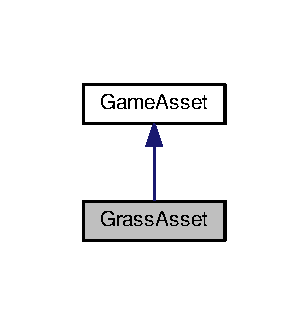
\includegraphics[width=148pt]{class_grass_asset__inherit__graph}
\end{center}
\end{figure}


Collaboration diagram for Grass\+Asset\+:
\nopagebreak
\begin{figure}[H]
\begin{center}
\leavevmode
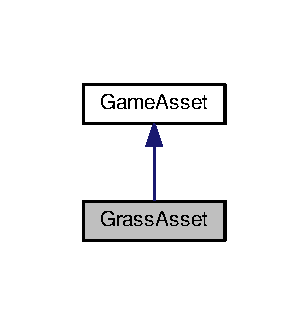
\includegraphics[width=148pt]{class_grass_asset__coll__graph}
\end{center}
\end{figure}
\subsection*{Public Member Functions}
\begin{DoxyCompactItemize}
\item 
\hyperlink{class_grass_asset_a6dd2fdfec9aa1396282f0711912b5740}{Grass\+Asset} (glm\+::vec3 xyz\+Position, glm\+::vec3 translate\+To, glm\+::vec3 animate\+To, bool translate\+\_\+bool, glm\+::vec3 rotate, bool rotate\+\_\+bool, glm\+::vec3 scale, bool scale\+\_\+bool, string Asset\+Type)
\item 
void \hyperlink{class_grass_asset_a0178a72c5bf2f00bcc6a240b851f3a25}{Draw} (G\+Luint)
\end{DoxyCompactItemize}


\subsection{Constructor \& Destructor Documentation}
\hypertarget{class_grass_asset_a6dd2fdfec9aa1396282f0711912b5740}{}\index{Grass\+Asset@{Grass\+Asset}!Grass\+Asset@{Grass\+Asset}}
\index{Grass\+Asset@{Grass\+Asset}!Grass\+Asset@{Grass\+Asset}}
\subsubsection[{Grass\+Asset(glm\+::vec3 xyz\+Position, glm\+::vec3 translate\+To, glm\+::vec3 animate\+To, bool translate\+\_\+bool, glm\+::vec3 rotate, bool rotate\+\_\+bool, glm\+::vec3 scale, bool scale\+\_\+bool, string Asset\+Type)}]{\setlength{\rightskip}{0pt plus 5cm}Grass\+Asset\+::\+Grass\+Asset (
\begin{DoxyParamCaption}
\item[{glm\+::vec3}]{xyz\+Position, }
\item[{glm\+::vec3}]{translate\+To, }
\item[{glm\+::vec3}]{animate\+To, }
\item[{bool}]{translate\+\_\+bool, }
\item[{glm\+::vec3}]{rotate, }
\item[{bool}]{rotate\+\_\+bool, }
\item[{glm\+::vec3}]{scale, }
\item[{bool}]{scale\+\_\+bool, }
\item[{string}]{Asset\+Type}
\end{DoxyParamCaption}
)}\label{class_grass_asset_a6dd2fdfec9aa1396282f0711912b5740}
model coordinates, origin at centre. Sets cordinates to a Grass/\+Pyramid with the center point 0.\+0 but moved to where the x, y, z variables calls them from the gameworld class through the G\+Lfloat x,y,z variables.

Color Buffer. Colour of Cube Asset Green Uses R\+G\+B values to set the colour.

\subsection{Member Function Documentation}
\hypertarget{class_grass_asset_a0178a72c5bf2f00bcc6a240b851f3a25}{}\index{Grass\+Asset@{Grass\+Asset}!Draw@{Draw}}
\index{Draw@{Draw}!Grass\+Asset@{Grass\+Asset}}
\subsubsection[{Draw(\+G\+Luint)}]{\setlength{\rightskip}{0pt plus 5cm}void Grass\+Asset\+::\+Draw (
\begin{DoxyParamCaption}
\item[{G\+Luint}]{program\+\_\+token}
\end{DoxyParamCaption}
)\hspace{0.3cm}{\ttfamily [virtual]}}\label{class_grass_asset_a0178a72c5bf2f00bcc6a240b851f3a25}
use the previously transferred buffer as the vertex array. This way we transfer the buffer once -- at construction -- not on every frame.

Uses the Previously transferred buffer as the color array. This way We transfer the buffer once -- at constuction -- not on every frame

Implements \hyperlink{class_game_asset}{Game\+Asset}.



The documentation for this class was generated from the following files\+:\begin{DoxyCompactItemize}
\item 
src/Grass\+Asset.\+h\item 
src/Grass\+Asset.\+cc\end{DoxyCompactItemize}

\hypertarget{class_ground_asset}{}\section{Ground\+Asset Class Reference}
\label{class_ground_asset}\index{Ground\+Asset@{Ground\+Asset}}


Inheritance diagram for Ground\+Asset\+:
\nopagebreak
\begin{figure}[H]
\begin{center}
\leavevmode
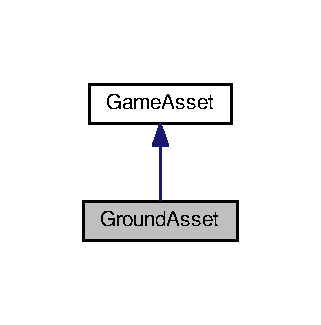
\includegraphics[width=154pt]{class_ground_asset__inherit__graph}
\end{center}
\end{figure}


Collaboration diagram for Ground\+Asset\+:
\nopagebreak
\begin{figure}[H]
\begin{center}
\leavevmode
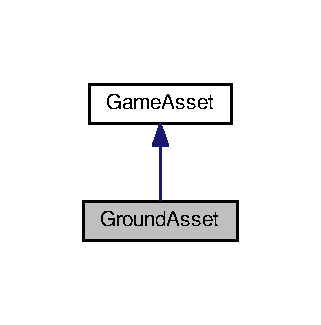
\includegraphics[width=154pt]{class_ground_asset__coll__graph}
\end{center}
\end{figure}
\subsection*{Public Member Functions}
\begin{DoxyCompactItemize}
\item 
\hyperlink{class_ground_asset_a67002eb5df923fab9293c5f43ed140a4}{Ground\+Asset} (glm\+::vec3 xyz\+Position, glm\+::vec3 translate\+To, glm\+::vec3 animate\+To, bool translate\+\_\+bool, glm\+::vec3 rotate, bool rotate\+\_\+bool, glm\+::vec3 scale, bool scale\+\_\+bool, string Asset\+Type)
\item 
void \hyperlink{class_ground_asset_a440f983638c7a7ccb6a39718444dfe95}{Draw} (G\+Luint)
\end{DoxyCompactItemize}


\subsection{Constructor \& Destructor Documentation}
\hypertarget{class_ground_asset_a67002eb5df923fab9293c5f43ed140a4}{}\index{Ground\+Asset@{Ground\+Asset}!Ground\+Asset@{Ground\+Asset}}
\index{Ground\+Asset@{Ground\+Asset}!Ground\+Asset@{Ground\+Asset}}
\subsubsection[{Ground\+Asset(glm\+::vec3 xyz\+Position, glm\+::vec3 translate\+To, glm\+::vec3 animate\+To, bool translate\+\_\+bool, glm\+::vec3 rotate, bool rotate\+\_\+bool, glm\+::vec3 scale, bool scale\+\_\+bool, string Asset\+Type)}]{\setlength{\rightskip}{0pt plus 5cm}Ground\+Asset\+::\+Ground\+Asset (
\begin{DoxyParamCaption}
\item[{glm\+::vec3}]{xyz\+Position, }
\item[{glm\+::vec3}]{translate\+To, }
\item[{glm\+::vec3}]{animate\+To, }
\item[{bool}]{translate\+\_\+bool, }
\item[{glm\+::vec3}]{rotate, }
\item[{bool}]{rotate\+\_\+bool, }
\item[{glm\+::vec3}]{scale, }
\item[{bool}]{scale\+\_\+bool, }
\item[{string}]{Asset\+Type}
\end{DoxyParamCaption}
)}\label{class_ground_asset_a67002eb5df923fab9293c5f43ed140a4}
model coordinates, origin at centre. Sets cordinates to a Cube with the center point 0.\+0 but moved to where the x, y, z variables calls them from the gameworld class through the G\+Lfloat x,y,z variables.

Color Buffer. Colour of Cube Lawn Green Uses R\+G\+B values to set the colour.

\subsection{Member Function Documentation}
\hypertarget{class_ground_asset_a440f983638c7a7ccb6a39718444dfe95}{}\index{Ground\+Asset@{Ground\+Asset}!Draw@{Draw}}
\index{Draw@{Draw}!Ground\+Asset@{Ground\+Asset}}
\subsubsection[{Draw(\+G\+Luint)}]{\setlength{\rightskip}{0pt plus 5cm}void Ground\+Asset\+::\+Draw (
\begin{DoxyParamCaption}
\item[{G\+Luint}]{program\+\_\+token}
\end{DoxyParamCaption}
)\hspace{0.3cm}{\ttfamily [virtual]}}\label{class_ground_asset_a440f983638c7a7ccb6a39718444dfe95}
use the previously transferred buffer as the vertex array. This way we transfer the buffer once -- at construction -- not on every frame.

Uses the Previously transferred buffer as the color array. This way We transfer the buffer once -- at constuction -- not on every frame

Implements \hyperlink{class_game_asset}{Game\+Asset}.



The documentation for this class was generated from the following files\+:\begin{DoxyCompactItemize}
\item 
src/Ground\+Asset.\+h\item 
src/Ground\+Asset.\+cc\end{DoxyCompactItemize}

\hypertarget{class_leaves_asset}{}\section{Leaves\+Asset Class Reference}
\label{class_leaves_asset}\index{Leaves\+Asset@{Leaves\+Asset}}


Inheritance diagram for Leaves\+Asset\+:
\nopagebreak
\begin{figure}[H]
\begin{center}
\leavevmode
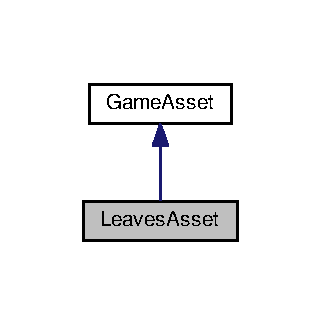
\includegraphics[width=154pt]{class_leaves_asset__inherit__graph}
\end{center}
\end{figure}


Collaboration diagram for Leaves\+Asset\+:
\nopagebreak
\begin{figure}[H]
\begin{center}
\leavevmode
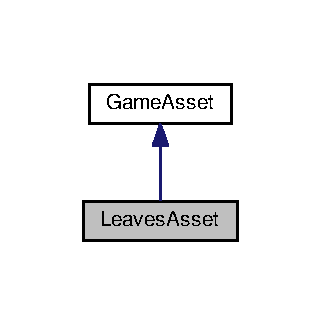
\includegraphics[width=154pt]{class_leaves_asset__coll__graph}
\end{center}
\end{figure}
\subsection*{Public Member Functions}
\begin{DoxyCompactItemize}
\item 
\hyperlink{class_leaves_asset_aa14436bbd45d5cce3e87bb79c2490a53}{Leaves\+Asset} (glm\+::vec3 xyz\+Position, glm\+::vec3 translate\+To, glm\+::vec3 animate\+To, bool translate\+\_\+bool, glm\+::vec3 rotate, bool rotate\+\_\+bool, glm\+::vec3 scale, bool scale\+\_\+bool, string Asset\+Type)
\item 
void \hyperlink{class_leaves_asset_a807fd196b83e5adb131d489ef6645742}{Draw} (G\+Luint)
\end{DoxyCompactItemize}


\subsection{Constructor \& Destructor Documentation}
\hypertarget{class_leaves_asset_aa14436bbd45d5cce3e87bb79c2490a53}{}\index{Leaves\+Asset@{Leaves\+Asset}!Leaves\+Asset@{Leaves\+Asset}}
\index{Leaves\+Asset@{Leaves\+Asset}!Leaves\+Asset@{Leaves\+Asset}}
\subsubsection[{Leaves\+Asset(glm\+::vec3 xyz\+Position, glm\+::vec3 translate\+To, glm\+::vec3 animate\+To, bool translate\+\_\+bool, glm\+::vec3 rotate, bool rotate\+\_\+bool, glm\+::vec3 scale, bool scale\+\_\+bool, string Asset\+Type)}]{\setlength{\rightskip}{0pt plus 5cm}Leaves\+Asset\+::\+Leaves\+Asset (
\begin{DoxyParamCaption}
\item[{glm\+::vec3}]{xyz\+Position, }
\item[{glm\+::vec3}]{translate\+To, }
\item[{glm\+::vec3}]{animate\+To, }
\item[{bool}]{translate\+\_\+bool, }
\item[{glm\+::vec3}]{rotate, }
\item[{bool}]{rotate\+\_\+bool, }
\item[{glm\+::vec3}]{scale, }
\item[{bool}]{scale\+\_\+bool, }
\item[{string}]{Asset\+Type}
\end{DoxyParamCaption}
)}\label{class_leaves_asset_aa14436bbd45d5cce3e87bb79c2490a53}
model coordinates, origin at centre. Sets cordinates to a Cube with the center point 0.\+0 but moved to where the x, y, z variables calls them from the gameworld class through the G\+Lfloat x,y,z variables.

Color Buffer. Colour of Cube Camerone Green \& Lawn Green Uses R\+G\+B values to set the colour.

\subsection{Member Function Documentation}
\hypertarget{class_leaves_asset_a807fd196b83e5adb131d489ef6645742}{}\index{Leaves\+Asset@{Leaves\+Asset}!Draw@{Draw}}
\index{Draw@{Draw}!Leaves\+Asset@{Leaves\+Asset}}
\subsubsection[{Draw(\+G\+Luint)}]{\setlength{\rightskip}{0pt plus 5cm}void Leaves\+Asset\+::\+Draw (
\begin{DoxyParamCaption}
\item[{G\+Luint}]{program\+\_\+token}
\end{DoxyParamCaption}
)\hspace{0.3cm}{\ttfamily [virtual]}}\label{class_leaves_asset_a807fd196b83e5adb131d489ef6645742}
use the previously transferred buffer as the vertex array. This way we transfer the buffer once -- at construction -- not on every frame.

Uses the Previously transferred buffer as the color array. This way We transfer the buffer once -- at constuction -- not on every frame

Implements \hyperlink{class_game_asset}{Game\+Asset}.



The documentation for this class was generated from the following files\+:\begin{DoxyCompactItemize}
\item 
src/Leaves\+Asset.\+h\item 
src/Leaves\+Asset.\+cc\end{DoxyCompactItemize}

\hypertarget{class_pyramid_asset}{}\section{Pyramid\+Asset Class Reference}
\label{class_pyramid_asset}\index{Pyramid\+Asset@{Pyramid\+Asset}}


{\ttfamily \#include $<$Pyramid\+Asset.\+h$>$}



Inheritance diagram for Pyramid\+Asset\+:\nopagebreak
\begin{figure}[H]
\begin{center}
\leavevmode
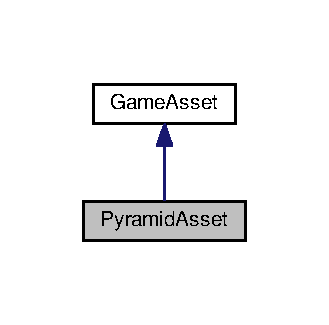
\includegraphics[width=158pt]{class_pyramid_asset__inherit__graph}
\end{center}
\end{figure}


Collaboration diagram for Pyramid\+Asset\+:\nopagebreak
\begin{figure}[H]
\begin{center}
\leavevmode
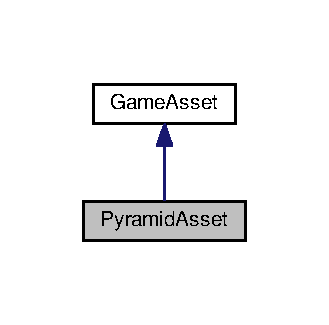
\includegraphics[width=158pt]{class_pyramid_asset__coll__graph}
\end{center}
\end{figure}
\subsection*{Public Member Functions}
\begin{DoxyCompactItemize}
\item 
\hyperlink{class_pyramid_asset_a6f20b7f915760ff772740f6c94c331b1}{Pyramid\+Asset} (glm\+::vec3 xyz\+Position, glm\+::vec3 translate\+To, glm\+::vec3 animate\+To, bool translate\+\_\+bool, glm\+::vec3 rotate, bool rotate\+\_\+bool, glm\+::vec3 scale, bool scale\+\_\+bool, string Asset\+Type)
\item 
\hyperlink{class_pyramid_asset_afb388a196f43a3808b2d4f6fdb89ee84}{$\sim$\+Pyramid\+Asset} ()
\item 
void \hyperlink{class_pyramid_asset_aaea45da4956d79ec9ab96e9d0ccef3fe}{Draw} (G\+Luint)
\end{DoxyCompactItemize}


\subsection{Constructor \& Destructor Documentation}
\hypertarget{class_pyramid_asset_a6f20b7f915760ff772740f6c94c331b1}{}\index{Pyramid\+Asset@{Pyramid\+Asset}!Pyramid\+Asset@{Pyramid\+Asset}}
\index{Pyramid\+Asset@{Pyramid\+Asset}!Pyramid\+Asset@{Pyramid\+Asset}}
\subsubsection[{Pyramid\+Asset(glm\+::vec3 xyz\+Position, glm\+::vec3 translate\+To, glm\+::vec3 animate\+To, bool translate\+\_\+bool, glm\+::vec3 rotate, bool rotate\+\_\+bool, glm\+::vec3 scale, bool scale\+\_\+bool, string Asset\+Type)}]{\setlength{\rightskip}{0pt plus 5cm}Pyramid\+Asset\+::\+Pyramid\+Asset (
\begin{DoxyParamCaption}
\item[{glm\+::vec3}]{xyz\+Position, }
\item[{glm\+::vec3}]{translate\+To, }
\item[{glm\+::vec3}]{animate\+To, }
\item[{bool}]{translate\+\_\+bool, }
\item[{glm\+::vec3}]{rotate, }
\item[{bool}]{rotate\+\_\+bool, }
\item[{glm\+::vec3}]{scale, }
\item[{bool}]{scale\+\_\+bool, }
\item[{string}]{Asset\+Type}
\end{DoxyParamCaption}
)}\label{class_pyramid_asset_a6f20b7f915760ff772740f6c94c331b1}
model coordinates, origin at centre. Sets cordinates to a Pyramid with the center point 0.\+0 but moved to where the x, y, z variables calls them from the gameworld class through the G\+Lfloat x,y,z variables.

Color Buffer. Colour of Cube Red, Green \& Blue. This creates a cool blend of colours Uses R\+G\+B values to set the colour.
\begin{DoxyCode}
7 : \hyperlink{class_game_asset_a9de932075d9b4263e7fb24fbfd163a61}{GameAsset}(xyzPosition, translateTo, animateTo , translate\_bool, rotate, rotate\_bool, scale,
      scale\_bool,AssetType) \{
8 
15   GLfloat vertex\_buffer [] \{
16       -0.5f + xyzPosition.x  , 0.0f + xyzPosition.y   ,-0.5f + xyzPosition.z
17      , 0.5f + xyzPosition.x  , 0.0f + xyzPosition.y   ,-0.5f + xyzPosition.z
18      ,-0.5f + xyzPosition.x  , 0.0f + xyzPosition.y   , 0.5f + xyzPosition.z
19      , 0.5f + xyzPosition.x  , 0.0f + xyzPosition.y   , 0.5f + xyzPosition.z
20      , 0.0f + xyzPosition.x  , 1.0f + xyzPosition.y   , 0.0f + xyzPosition.z
21   \};
22   GLfloat vertex\_buffer\_length = \textcolor{keyword}{sizeof}(vertex\_buffer);
28   GLfloat colour\_buffer[] = \{
29 
30      1.000f, 0.000f, 0.000f,
31      0.000f, 1.000f, 0.000f,
32      0.000f, 0.000f, 1.000f,
33      1.000f, 0.000f, 0.000f,
34      0.000f, 1.000f, 0.000f,
35      0.000f, 0.000f, 1.000f,
36      1.000f, 0.000f, 0.000f,
37      0.000f, 1.000f, 0.000f,
38      0.000f, 0.000f, 1.000f
39   \};
40  colour\_buffer\_length = \textcolor{keyword}{sizeof}(colour\_buffer);
41   
42   GLuint element\_buffer []  \{
43       0, 4, 1   
44     , 1, 4, 3
45     , 2, 4, 3   
46     , 2, 4, 0
47     , 0, 2, 1
48     , 1, 2, 3
49   \};
50   element\_buffer\_length = \textcolor{keyword}{sizeof}(element\_buffer);
51 
52 
53 
54   \textcolor{comment}{// Transfer buffers to the GPU}
55 
56   \textcolor{comment}{// create buffer}
57   glGenBuffers(1, &vertex\_buffer\_token);
58   \textcolor{comment}{// immediately bind the buffer and transfer the data}
59   glBindBuffer(GL\_ARRAY\_BUFFER, vertex\_buffer\_token);
60   glBufferData(GL\_ARRAY\_BUFFER, vertex\_buffer\_length, vertex\_buffer, GL\_STATIC\_DRAW);
61 
62   \textcolor{comment}{// Binds the buffer and transfers the data}
63   glGenBuffers(1, &colour\_buffer\_token);
64   glBindBuffer(GL\_ARRAY\_BUFFER, colour\_buffer\_token);
65   glBufferData(GL\_ARRAY\_BUFFER, colour\_buffer\_length, colour\_buffer, GL\_STATIC\_DRAW);
66 
67 
68   glGenBuffers(1, &element\_buffer\_token);
69   glBindBuffer(GL\_ELEMENT\_ARRAY\_BUFFER, element\_buffer\_token);
70   glBufferData(GL\_ELEMENT\_ARRAY\_BUFFER, element\_buffer\_length, element\_buffer, GL\_STATIC\_DRAW);
71 \}
\end{DoxyCode}
\hypertarget{class_pyramid_asset_afb388a196f43a3808b2d4f6fdb89ee84}{}\index{Pyramid\+Asset@{Pyramid\+Asset}!````~Pyramid\+Asset@{$\sim$\+Pyramid\+Asset}}
\index{````~Pyramid\+Asset@{$\sim$\+Pyramid\+Asset}!Pyramid\+Asset@{Pyramid\+Asset}}
\subsubsection[{$\sim$\+Pyramid\+Asset()}]{\setlength{\rightskip}{0pt plus 5cm}Pyramid\+Asset\+::$\sim$\+Pyramid\+Asset (
\begin{DoxyParamCaption}
{}
\end{DoxyParamCaption}
)}\label{class_pyramid_asset_afb388a196f43a3808b2d4f6fdb89ee84}

\begin{DoxyCode}
73                             \{
74 \}
\end{DoxyCode}


\subsection{Member Function Documentation}
\hypertarget{class_pyramid_asset_aaea45da4956d79ec9ab96e9d0ccef3fe}{}\index{Pyramid\+Asset@{Pyramid\+Asset}!Draw@{Draw}}
\index{Draw@{Draw}!Pyramid\+Asset@{Pyramid\+Asset}}
\subsubsection[{Draw(\+G\+Luint)}]{\setlength{\rightskip}{0pt plus 5cm}void Pyramid\+Asset\+::\+Draw (
\begin{DoxyParamCaption}
\item[{G\+Luint}]{program\+\_\+token}
\end{DoxyParamCaption}
)\hspace{0.3cm}{\ttfamily [virtual]}}\label{class_pyramid_asset_aaea45da4956d79ec9ab96e9d0ccef3fe}
use the previously transferred buffer as the vertex array. This way we transfer the buffer once -- at construction -- not on every frame.

Uses the Previously transferred buffer as the color array. This way We transfer the buffer once -- at constuction -- not on every frame

Implements \hyperlink{class_game_asset_a961aa51ca0a9961fc584c0b5d5431300}{Game\+Asset}.


\begin{DoxyCode}
83                                             \{
84   \textcolor{keywordflow}{if}(!glIsProgram(program\_token)) \{
85     \textcolor{comment}{//std::cerr << "Drawing Pyramid with invalid program" << std::endl;}
86     \textcolor{keywordflow}{return};
87   \}
88   GLint validation\_ok;
89   glValidateProgram(program\_token);
90   glGetProgramiv(program\_token, GL\_VALIDATE\_STATUS, &validation\_ok);
91   \textcolor{keywordflow}{if}(!validation\_ok) \{
92     GLint maxLength = 0;
93     glGetProgramiv(program\_token, GL\_INFO\_LOG\_LENGTH, &maxLength);
94 
95     \textcolor{comment}{// The maxLength includes the NULL character}
96     std::vector<char> errorLog(maxLength);
97     glGetProgramInfoLog(program\_token, maxLength, &maxLength, &errorLog[0]);
98 
99     std::cerr << \textcolor{stringliteral}{"Invalid program "} << program\_token << \textcolor{stringliteral}{" with error code "} << validation\_ok << std::endl;
100     \textcolor{keywordflow}{for}(\textcolor{keyword}{auto} c: errorLog) \{
101       std::cerr << c;
102     \}
103     exit(-1);
104   \}
105 
106   GLuint position\_attrib = glGetAttribLocation(program\_token, \textcolor{stringliteral}{"position"});
107   \hyperlink{_pyramid_asset_8cc_a75f201b0e53e68726854997957322b8d}{checkGLError}();
108 
109   glUseProgram(program\_token);
110   \hyperlink{_pyramid_asset_8cc_a75f201b0e53e68726854997957322b8d}{checkGLError}();
111 
116   glEnableVertexAttribArray(0);
117   glBindBuffer(GL\_ARRAY\_BUFFER, vertex\_buffer\_token);
118   glVertexAttribPointer(
119     position\_attrib,        \textcolor{comment}{/* attribute */}
120     3,        \textcolor{comment}{/* size */}
121     GL\_FLOAT,   \textcolor{comment}{/* type */}
122     GL\_FALSE,   \textcolor{comment}{/* normalized? */}
123     0,        \textcolor{comment}{/* stride */}
124     (\textcolor{keywordtype}{void}*)0    \textcolor{comment}{/* array buffer offset */}
125   );
126   glEnableVertexAttribArray(1);
127   \hyperlink{_pyramid_asset_8cc_a75f201b0e53e68726854997957322b8d}{checkGLError}();
132   glBindBuffer(GL\_ARRAY\_BUFFER, colour\_buffer\_token);
133   glVertexAttribPointer(
134     1,        \textcolor{comment}{/* attribute */}
135     3,        \textcolor{comment}{/* size */}
136     GL\_FLOAT,   \textcolor{comment}{/* type */}
137     GL\_FALSE,   \textcolor{comment}{/* normalized? */}
138     0,        \textcolor{comment}{/* stride */}
139     (\textcolor{keywordtype}{void}*)0    \textcolor{comment}{/* array buffer offset */}
140   );
141   \hyperlink{_pyramid_asset_8cc_a75f201b0e53e68726854997957322b8d}{checkGLError}();
142 
143   glBindBuffer(GL\_ELEMENT\_ARRAY\_BUFFER, element\_buffer\_token);
144   glDrawElements(
145     GL\_TRIANGLES,
146     element\_buffer\_length,
147     GL\_UNSIGNED\_INT,
148     (GLvoid*) 0
149   );
150   \hyperlink{_pyramid_asset_8cc_a75f201b0e53e68726854997957322b8d}{checkGLError}();
151 
152   glDisableVertexAttribArray(position\_attrib);
153 \}
\end{DoxyCode}


The documentation for this class was generated from the following files\+:\begin{DoxyCompactItemize}
\item 
src/\hyperlink{_pyramid_asset_8h}{Pyramid\+Asset.\+h}\item 
src/\hyperlink{_pyramid_asset_8cc}{Pyramid\+Asset.\+cc}\end{DoxyCompactItemize}

\hypertarget{class_python_bind}{}\section{Python\+Bind Class Reference}
\label{class_python_bind}\index{Python\+Bind@{Python\+Bind}}


{\ttfamily \#include $<$Python\+Bind.\+h$>$}

\subsection*{Public Member Functions}
\begin{DoxyCompactItemize}
\item 
\hyperlink{class_python_bind_a6fa707a0f4e8f4363fccf75c2caf508f}{Python\+Bind} ()
\end{DoxyCompactItemize}
\subsection*{Public Attributes}
\begin{DoxyCompactItemize}
\item 
tuple \hyperlink{class_python_bind_a58a0da72b60d10ef74d6d572b158d30a}{Run} = libglex.\+Game\+Loop()
\end{DoxyCompactItemize}


\subsection{Constructor \& Destructor Documentation}
\hypertarget{class_python_bind_a6fa707a0f4e8f4363fccf75c2caf508f}{}\index{Python\+Bind@{Python\+Bind}!Python\+Bind@{Python\+Bind}}
\index{Python\+Bind@{Python\+Bind}!Python\+Bind@{Python\+Bind}}
\subsubsection[{Python\+Bind()}]{\setlength{\rightskip}{0pt plus 5cm}Python\+Bind\+::\+Python\+Bind (
\begin{DoxyParamCaption}
{}
\end{DoxyParamCaption}
)}\label{class_python_bind_a6fa707a0f4e8f4363fccf75c2caf508f}

\begin{DoxyCode}
5                       \{
6 
7 \}
\end{DoxyCode}


\subsection{Member Data Documentation}
\hypertarget{class_python_bind_a58a0da72b60d10ef74d6d572b158d30a}{}\index{Python\+Bind@{Python\+Bind}!Run@{Run}}
\index{Run@{Run}!Python\+Bind@{Python\+Bind}}
\subsubsection[{Run}]{\setlength{\rightskip}{0pt plus 5cm}tuple Python\+Bind.\+Run = libglex.\+Game\+Loop()}\label{class_python_bind_a58a0da72b60d10ef74d6d572b158d30a}


The documentation for this class was generated from the following files\+:\begin{DoxyCompactItemize}
\item 
src/\hyperlink{_python_bind_8h}{Python\+Bind.\+h}\item 
src/\hyperlink{_python_bind_8py}{Python\+Bind.\+py}\item 
src/\hyperlink{_python_bind_8cc}{Python\+Bind.\+cc}\end{DoxyCompactItemize}

\hypertarget{struct_s_d_l_window_deleter}{}\section{S\+D\+L\+Window\+Deleter Struct Reference}
\label{struct_s_d_l_window_deleter}\index{S\+D\+L\+Window\+Deleter@{S\+D\+L\+Window\+Deleter}}
\subsection*{Public Member Functions}
\begin{DoxyCompactItemize}
\item 
void \hyperlink{struct_s_d_l_window_deleter_a2aedcc99c3756ae090c38badabeb10b1}{operator()} (S\+D\+L\+\_\+\+Window $\ast$window)
\end{DoxyCompactItemize}


\subsection{Member Function Documentation}
\hypertarget{struct_s_d_l_window_deleter_a2aedcc99c3756ae090c38badabeb10b1}{}\index{S\+D\+L\+Window\+Deleter@{S\+D\+L\+Window\+Deleter}!operator()@{operator()}}
\index{operator()@{operator()}!S\+D\+L\+Window\+Deleter@{S\+D\+L\+Window\+Deleter}}
\subsubsection[{operator()(\+S\+D\+L\+\_\+\+Window $\ast$window)}]{\setlength{\rightskip}{0pt plus 5cm}void S\+D\+L\+Window\+Deleter\+::operator() (
\begin{DoxyParamCaption}
\item[{S\+D\+L\+\_\+\+Window $\ast$}]{window}
\end{DoxyParamCaption}
)\hspace{0.3cm}{\ttfamily [inline]}}\label{struct_s_d_l_window_deleter_a2aedcc99c3756ae090c38badabeb10b1}

\begin{DoxyCode}
23                                                    \{
24                 SDL\_DestroyWindow(window);
25         \}
\end{DoxyCode}


The documentation for this struct was generated from the following file\+:\begin{DoxyCompactItemize}
\item 
src/\hyperlink{_game_loop_8cc}{Game\+Loop.\+cc}\end{DoxyCompactItemize}

%--- End generated contents ---

% Index
\backmatter
\newpage
\phantomsection
\clearemptydoublepage
\addcontentsline{toc}{chapter}{Index}
\printindex

\end{document}
